% Template:     Tesis LaTeX
% Documento:    Archivo principal
% Versión:      3.4.2 (07/02/2025)
% Codificación: UTF-8
%
% Autor: Pablo Pizarro R.
%        pablo@ppizarror.com
%
% Manual template: [https://latex.ppizarror.com/tesis]
% Licencia MIT:    [https://opensource.org/licenses/MIT]

% CREACIÓN DEL DOCUMENTO
\documentclass[
	spanish, % Idioma: spanish, english, etc.	
	letterpaper, oneside
]{book}
\usepackage{tikz}
\usetikzlibrary{arrows.meta,positioning,shapes.geometric,calc}
\usetikzlibrary{positioning, arrows.meta, shapes.geometric, matrix}
\usetikzlibrary{positioning, arrows.meta, shapes.geometric, fit, backgrounds}
\usetikzlibrary{positioning, arrows.meta, fit, backgrounds}
\usepackage{parskip}



% INFORMACIÓN DEL DOCUMENTO
\def\documenttitle {Explainable Brain Tumor Classification via Generation Using Conditional StyleGANs and CNNs}
\def\documentsubtitle {}
\def\degreetitle {
	Tesis para optar al grado de magíster en ciencia de datos
	\bigbreak\vspace{0.3cm}
	Memoria para optar al título de ingeniero civil industrial
}

\def\universityname {Universidad de Chile}
\def\universityfaculty {Facultad de Ciencias Físicas y Matemáticas}
\def\universitydepartment {ESCUELA DE POSTGRADO Y EDUCACIÓN CONTINUA \\ Departamento de Ingeniería Industrial}
\def\universitydepartmentimage {departamentos/uchile2}
\def\universitydepartmentimagecfg {height=3cm}
\def\universitylocation {Santiago de Chile}

% INTEGRANTES, PROFESORES Y FECHAS
\def\documentauthor {Junwei He Mai}
\def\documentdate {\the\year}

\def\portrait {
	\begin{center}
	\vspace{1.5cm} ~ \\
	\MakeUppercase{\textbf{\documenttitle}} ~ \\
	\vspace{1.5cm}
	\MakeUppercase{\degreetitle} ~ \\
	\vfill
	\begin{tabular}{c}
		\MakeUppercase{\textbf{\documentauthor}} \\ \\
		\vspace{1.0cm} \\
		PROFESOR GUÍA: \\
		JUAN VELÁSQUEZ SILVA\\
        \vspace{0.2cm} \\
        PROFESOR CO-GUÍA: \\
		YONG ZHANG \\
        \vspace{0.5cm} \\
		MIEMBROS DE LA COMISIÓN: \\
		INGEBORG LÓPEZ LIBERONA \\
		DENIS SAURÉ VALENZUELA \\
        \vspace{0.5cm} \\
		\MakeUppercase{\universitylocation} \\
		\MakeUppercase{\documentdate}
	\end{tabular}
	\end{center}
}




% IMPORTACIÓN DEL TEMPLATE
\input{template}

% INICIO DE LAS PÁGINAS
\begin{document}

% PORTADA
\templatePortrait

% CONFIGURACIÓN DE PÁGINA Y ENCABEZADOS
\templatePagecfg

% RESUMEN O ABSTRACT

\begin{abstractd}
Brain tumors, including gliomas, meningiomas, and pituitary tumors, represent a major health issue due to their high mortality rate. Unlike other medical imaging domains, brain tumor MRI classification is particularly challenging due to the high inter-class visual similarity between tumor types (e.g., glioma vs.\ meningioma), the heterogeneous appearance of lesions across patients and acquisition protocols, and the limited availability of large-scale, patient-annotated public datasets. This thesis addresses the implementation of deep learning models for the classification of these tumors while ensuring strict control of data leakage between patients. Initially, an image generator is trained to create synthetic images of the desired tumor types, achieving a Fr\’echet Inception Distance (FID) of 46.08 (lower is better) and a 0.50 diagnostic accuracy by medical experts on the synthetic images, indicating that approximately half of the generated images reached sufficient quality for clinical interpretation while the remainder were deemed non-diagnostic --- a finding that highlights the current limitations of generative models in medical imaging. The Classification Accuracy Score (CAS) metric shows an accuracy of 0.923 for classifying these synthetic images. Different classification approaches are then explored, including latent space inversion with an accuracy of 0.832 using the e4e encoder, 0.838 through optimization, and 0.960 using a Convolutional Neural Network (CNN) with augmented synthetic data. eXplainable AI (XAI) techniques, such as heatmaps, are implemented to identify the most influential regions in the classifier’s decision-making process. For synthetic images, expert diagnostic confidence increased from 1.44 to 3.0 on the Likert scale when utilizing these maps. This thesis establishes a foundation for future research by introducing more stringent data leakage control and proposing new evaluation metrics such as CAS. Additionally, the integration of Human-in-the-Loop (HITL) is recommended for evaluating both augmented images and model decisions, leveraging XAI methods to provide interpretable insights. Finally, statistical tests are suggested to validate the differences between the models.\\

\textbf{Keywords}: Brain Tumor Classification, StyleGAN, Synthetic Data Augmentation, Explainable AI, Data Leakage Control
\end{abstractd}


\renewcommand{\documenttitle}{Clasificación Explicable de Tumores Cerebrales mediante Generación con StyleGAN Condicional y Redes Neuronales Convolucionales}
\begin{abstractd}
Los tumores cerebrales, incluyendo gliomas, meningiomas y tumores pituitarios, representan un problema de salud importante debido a su alta tasa de mortalidad. A diferencia de otros dominios de imagen médica, la clasificación de tumores cerebrales por MRI es particularmente desafiante debido a la alta similitud visual entre tipos de tumor, la apariencia heterogénea de las lesiones entre pacientes y protocolos de adquisición, y la limitada disponibilidad de conjuntos de datos públicos anotados a nivel de paciente. Esta tesis aborda la implementación de modelos de \textit{deep learning} para la clasificación de estos tumores, asegurando un estricto control de fuga de datos entre pacientes. Primero, se entrena un generador de imágenes que permite la creación de imágenes sintéticas de los tipos de tumor deseados, logrando un \textit{Fr\'echet Inception Distance} (FID) de 46.08 (menor es mejor) y una precisión de 0.50 en el diagnóstico por parte de expertos médicos sobre las imágenes sintéticas, lo que indica que aproximadamente la mitad de las imágenes generadas alcanzaron calidad suficiente para interpretación clínica mientras que el resto fueron consideradas no diagnósticas --- un hallazgo que subraya las limitaciones actuales de los modelos generativos en imagen médica. La métrica \textbf{Classification Accuracy Score (CAS)} muestra una precisión de 0.923 para la clasificación de estas imágenes sintéticas. Luego, se exploran diferentes enfoques para clasificar estos tumores, incluyendo la inversión del espacio latente con un \textit{accuracy} de 0.832 utilizando el encoder \textit{e4e}, de 0.838 mediante optimización, y de 0.960 utilizando una Convolutional Neural Network (CNN) con datos sintéticos aumentados. Se implementan técnicas de eXplainable AI (XAI), como los mapas de calor, para identificar las regiones más influyentes en el proceso de toma de decisiones del clasificador. Para las imágenes sintéticas, la confianza diagnóstica del experto aumentó de 1.44 a 3.0 en la escala de Likert al utilizar estos mapas. Esta tesis establece una base para futuras investigaciones integrando un control más estricto de fuga de datos y proponiendo nuevas métricas de evaluación como el CAS. Además, se recomienda la integración de \textit{Human-in-the-Loop} (HITL) para evaluar tanto las imágenes utilizadas en el proceso de \textit{augmentación} como las decisiones tomadas por estos modelos de caja negra, aprovechando las técnicas de XAI para proporcionar interpretaciones claras y comprensibles. Por último, se sugiere la implementación de pruebas estadísticas para validar las diferencias entre los modelos.\\

\textbf{Keywords}: Brain Tumor Classification, StyleGAN, Synthetic Data Augmentation, Explainable AI, Data Leakage Control


\end{abstractd}
\renewcommand{\documenttitle}{Explainable Brain Tumor Classification via Generation Using Conditional StyleGANs and CNNs}


% DEDICATORIA
\begin{dedicatory}
	Para mi familia que lo ha dado todo por mi. \\	~ \\
\end{dedicatory}

% AGRADECIMIENTOS
\begin{acknowledgments}

Terminar esta tesis significa cumplir y culminar un ciclo que no empieza en la universidad, sino de mucho más atrás. Un proceso que nos llevó más de una década y finalmente se pudo lograr gracias a mi familia y principalmente a mi mamá, que me pudo otorgar todas las herramientas y facilidades para poder llegar hasta acá. Soy muy consciente y estoy muy agradecido del enorme esfuerzo por todo el apoyo que me han dado.\\

Quiero ofrecer mi agradecimiento a todos los compañeros que me ayudaron a lo largo de la carrera. Tuve una suerte tremenda al coincidir grandes personas que no se molestaron ni un momento en prestarme ayuda. Mis amigos Gustavo e Ignacio que siempre estuvieron ahí para cualquier cosa. Los sureños Kalen, Joaco y a todos los de la rama que siempre me acompañaron con el pinpon. Y muchas otras más personas que hicieron mi carrera mucho más divertida.\\

En tercer lugar quiero agradecer a la Universidad de Chile, al departamento de Industrias y al Magister de Ciencia de Datos, por todos los conocimientos que me ha brindado gracias a su enorme planta de profesores de altisima calidad.\\

A la doctora Ingeborg por su tiempo y dedicación para aportar una mirada clínica al proyecto que fue fundamental para respaldar los resultados.\\

Por último, muchas gracias a mis profesores Juan Velásquez y Yong Zhang por confiar en mi y guiarme durante todo el proceso. Valoro mucho el tiempo y la disposición a pesar de la gran diferencia horaria.
\end{acknowledgments}

% TABLA DE CONTENIDOS - ÍNDICE
\templateIndex

% CONFIGURACIONES FINALES
\templateFinalcfg

% ======================= INICIO DEL DOCUMENTO =======================

\chapter{Introduction}

This chapter presents the context and motivation of the study, along with the research questions, working hypotheses, and general objectives. It also outlines the overall strategy and methodology, describing how the proposed components are interconnected. Finally, it previews the main contributions and offers a road map for the remainder of the thesis within its scientific and clinical context. This thesis focuses on integrating class conditional MRI generation with classifier training under strict patient level data leakage control.

\section{Background and Motivation}

Brain tumors constitute a major neurological burden due to their high morbidity, mortality, and long-term functional impact. Early and reliable diagnosis is crucial for treatment planning, surgical decision-making, and follow-up, as prognosis and therapeutic strategies strongly depend on tumor type \cite{Vadhavekar2024AdvancementsImagingNeurosurgical}. Magnetic Resonance Imaging (MRI) is the primary non-invasive modality for brain tumor assessment because of its high soft-tissue contrast and multiplanar characterization capabilities. Nevertheless, clinical interpretation remains time consuming and subject to inter observer variability, particularly when tumors exhibit subtle borders, heterogeneous appearance, or overlap in radiological patterns across classes.\\

In recent years, deep learning methods especially Convolutional Neural Networks (CNNs) \cite{hayat2024cnnsvm} have shown strong performance in brain tumor recognition from MRI slices. These models can learn discriminative features directly from images, often reaching high accuracy on public benchmarks. However, most existing approaches are purely discriminative and provide limited interpretability, offering clinicians little evidence beyond a predicted label. In high stakes medical settings, such opacity can reduce trust and hinder adoption, particularly when automated predictions conflict with clinical judgment.\\

A second critical limitation in this field is the scarcity and limited diversity of public MRI datasets. Many studies rely on a small number of widely reused cohorts. As a result, models may overfit dataset specific characteristics and exhibit substantial performance drops under domain shift, when deployed on images from different hospitals, scanners, or acquisition settings. In addition, progress is further constrained by the lack of publicly available datasets with reliable patient level annotation. Most resources do not provide detailed per-patient metadata and are reused extensively without clear documentation of how patients are split across partitions. This leads to a common methodological flaw: data leakage, whereby MRI slices from the same patient appear in both training and test sets. Because a single patient may contribute multiple highly correlated slices across axial, sagittal, and coronal planes, models can learn to recognize patient-specific anatomical features rather than tumor-specific characteristics, leading to artificially inflated accuracy. This thesis enforces strict patient-disjoint partitions throughout all experiments to prevent this form of leakage. Such leakage inflates performance metrics and undermines the clinical validity of the reported results, making rigorous patient-level separation and explicit duplicate control essential to obtain generalizable and trustworthy conclusions.\\



Generative models offer a promising avenue to address these challenges. Among them, StyleGAN-based architectures provide notable advantages over traditional GANs due to their disentangled latent space ($\mathcal{W}$) \cite{karras2019stylebasedgeneratorarchitecturegenerative}, which enables controlled semantic manipulation and high quality image reconstruction. These properties are particularly beneficial for inference by generation approaches, where a query image is inverted into latent space and compared to class conditional reconstructions to provide structural evidence for classification. \\


In addition, StyleGAN models can be leveraged to augment limited training datasets, potentially enhancing robustness under patient level evaluation. However, for these models to gain clinical acceptance, their outputs must be validated not only through automated metrics but also via expert human in the loop (HITL) assessment, focusing on both realism and diagnostic utility. In this work, \textbf{StyleGAN-C} denotes a class conditional extension of StyleGAN2-ADA, adapted for brain tumor MRI synthesis. The model incorporates class specific embeddings and includes minor architectural refinements to better align with clinical plausibility standards in medical imaging. Compared to alternative generative frameworks such as diffusion models or variational autoencoders (VAEs), StyleGAN-C is preferred due to its structured latent spaces ($\mathcal{W}/\mathcal{W}^+$), which support rapid class-conditional inversion and enable semantically meaningful image manipulation, as well as its StyleGAN2-ADA backbone, which offers a favorable trade-off between training speed, sample quality, and computational cost \cite{abdullah2025computationallyefficientdiffusionmodels}.
These properties are critical for realistic class-conditional MRI image generation, the inference by generation proposed strategy, and the counterfactual explainability mechanisms proposed in this thesis.\\

Motivated by these gaps, this thesis proposes an explainable brain tumor classification framework composed of three integrated components: (i) generation of clinically validated class-conditional MRI images using StyleGAN-C, (ii) a classification strategy that uses StyleGAN-C to classify brain tumor MRI images, and (iii) an image-based XAI module that enables clinicians to interpret model predictions in a clinically meaningful way.\\



\section{Research Questions}
\begin{enumerate}
    \item \textbf{Generative validity:} 
       Do class conditional MRI images generated by StyleGAN-C reach clinically acceptable levels of realism and diagnostic utility, as determined by neuroradiologist HITL ratings using structured Likert-style forms?


    \item \textbf{Impact of StyleGAN-C on classification methods:} 
    How does incorporating StyleGAN-C affect brain tumor MRI classification when used through 
    (i) inference-by-generation via latent inversion and perceptual similarity, and 
    (ii) synthetic data augmentation for CNN training?

    \item \textbf{Image-based explainability:} 
    Can image-based explainability methods that incorporate generative evidence provide clinically interpretable visual support that assists neuroradiologists in the diagnostic process? 

\end{enumerate}

\section{Hypotheses}




\begin{itemize}
    \item H1: StyleGAN-C generates class conditional brain tumor MRI slices that preserve the relevant tumor-related anatomical structures, as reflected by high neuroradiologist HITL ratings.

    
    \item H2A: Using optimization or encoder based latent inversion in the StyleGAN-C latent space enables tumor classification with an accuracy above 0.8.

    
    \item H2B: Incorporating StyleGAN-C generated synthetic images into the training set of a CNN classifier improves the confidence of its probabilistic predictions compared to a model trained exclusively on real MRI images.
    
    
    \item H3: Image based explainability methods provide neuroradiologists with more clinically useful and trustworthy support for brain tumor classification than not using such methods.

\end{itemize}

The hypotheses encompass both conceptual and operational aspects. H1 and H3 are primarily conceptual, as they focus on clinical plausibility and perceived usefulness evaluated through expert assessment. In contrast, H2A and H2B are operational hypotheses, tested using quantitative performance metrics such as accuracy and predictive confidence.

\section{Objectives}

\subsection{General Objective}
To develop and evaluate an explainable brain tumor MRI classification framework built on three integrated pillars: (i) generation of clinically validated class-conditional MRI images using StyleGAN-C, (ii) a classification strategy that uses StyleGAN-C to classify brain tumor MRI images, and (iii) an image based XAI module that enables clinicians to interpret model predictions in a clinically meaningful way.


\subsection{Specific Objectives}

\begin{enumerate}

    \item To enforce patient level data leakage control in all experiments, ensuring that no subject appears across splits and that reported performance reflects clinically realistic generalization.

    \item To implement and train a StyleGAN-C model for generating class-conditional synthetic brain tumor MRI images conditioned on tumor type.

    \item To develop and evaluate an inference by generation classifier using StyleGAN-C latent inversion and perceptual similarity, and to compare this approach against a supervised discriminative encoder baseline.

    \item To train and evaluate both a supervised encoder and an e4e based encoder that map real MRI slices into the latent space.
    
    \item To design, implement, and train a CNN baseline classifier for brain tumor classification from real MRI images under patient level cross-validation.
    
    \item To investigate how StyleGAN-C truncation and class-conditional synthetic augmentation influence classification accuracy and model robustness, incorporating statistical analysis and ablation studies to rigorously support the observed effects.

    \item To generate image-based explanations for classification decisions and clinically validate the quality and usefulness of the generated images through expert review by neuroradiologists in order to improve interpretability.

\end{enumerate}


\begin{table}[ht]
\centering
\caption{Mapping of Specific Objectives to Experiments}
\begin{tabular}{|p{6.5cm}|p{2.5cm}|p{3cm}|}
\hline
\textbf{Objective} & \textbf{Research Question} & \textbf{Experiment(s)} \\
\hline
Obj. 1: Enforce patient-level data leakage control & RQ1, RQ2, RQ3 & All experiments \\
\hline
Obj. 2: Train StyleGAN-C for conditional generation & RQ1 & Experiment 1 \\
\hline
Obj. 3: Evaluate inference-by-generation & RQ2 & Experiment 2A \\
\hline
Obj. 4: Train supervised and e4e-based encoders & RQ2 & Experiment 2B \\
\hline
Obj. 5: Train CNN classifier & RQ2 & Experiments 2A, 2B, 2C \\
\hline
Obj. 6: Analyze the effect of truncation and GAN-based augmentation using ablation studies and statistical tests & RQ2 & Experiment 2C \\
\hline
Obj. 7: Generate and clinically validate image-based explanations & RQ3 & Experiment 3 \\
\hline
\end{tabular}
\label{tab:objectives_mapping}
\end{table}

Table~\ref{tab:objectives_mapping} summarizes the correspondence between the research objectives and the experiments conducted throughout this thesis. Despite addressing distinct methodological components, the three experiments are cohesively integrated into a \textbf{single end-to-end framework} spanning image generation (Experiment~1), predictive classification (Experiment~2), and clinical-level explainability (Experiment~3). In particular, Experiment~1 does not conceive generation as an end in itself, but rather as an \textbf{epistemological instrument} that enables the rest of the methodological pipeline: it allows (i) the evaluation of clinical plausibility and structural coherence of generated images, (ii) the implementation of \emph{classification by generation} through latent inference, and (iii) the enhancement of discriminative models under realistic scenarios of data scarcity, class imbalance, and strict patient-level data leakage control. From this perspective, the three experiments should be interpreted as interdependent components of a unified methodological approach, rather than as isolated evaluations of independent techniques.


\clearpage

\section{Methodology}

The methodology designed to achieve the specific objectives of this thesis is organized into three main stages:

\begin{enumerate}
    \item \textbf{Dataset and Preprocessing}
    \begin{itemize}
        \item \textbf{Data Collection and Preprocessing:} Integrate the Figshare public MRI brain tumor dataset \cite{Cheng2015}, ensuring coverage of different tumor types and imaging modalities. Then, apply a preprocessing pipeline.

        \item \textbf{Patient-Level Splitting and Leakage Control:} Create training and testing splits using unique patients, ensuring that no subject appears in more than one partition.

        \item \textbf{Patient-Level Cross-Validation:} Within the training pool, perform k-fold cross-validation at the patient level, ensuring that each fold contains a disjoint set of patients and that no subject appears across folds.

    \end{itemize}

    \item \textbf{Design and Training}
    \begin{itemize}
        \item \textbf{Generative Models:} Implement and train a StyleGAN-C to learn a class-conditional generative space and produce high-quality synthetic MRI images conditioned on tumor type.

        \item \textbf{CNN Classifier:} Implement and train a CNN baseline for brain tumor classification using both real and StyleGAN-C augmented datasets. Robustness is strengthened through patient-level k-fold cross-validation and ablation studies over key hyperparameters and training variables.

        \item \textbf{Classification by Generation Framework:} Design a classification by generation approach in which each input MRI slice is mapped to latent space, modified to generate class-conditional reconstructions for each tumor type, and compared to the original image using LPIPS or CNN.

        \item \textbf{e4e Latent Inversion:} Integrate and train an e4e encoder to invert MRI slices into latent space.

    \end{itemize}

    \item \textbf{Human in the Loop (HITL) Evaluation}
    \begin{itemize}
        \item \textbf{Explainability and Visual Explanations:}  Generate image-based explanations to provide clinically interpretable support for predictions.

        \item \textbf{Validation and Clinical Feedback:} Validate the clinical quality of generated images through expert review by neuroradiologists, using HITL rating forms that assess realism, image quality, and diagnostic usefulness.


    \end{itemize}
\end{enumerate}
\section{Contribution}
\begin{enumerate}



\item Developed and evaluated a CNN ensemble approach for brain tumor MRI classification, demonstrating a performance improvement from an accuracy of 0.934 in a single-run baseline trained exclusively on real images to 0.960 in an ensemble trained with StyleGAN-C augmented data.

\item Developed and clinically validated a class-conditional StyleGAN-C generator for brain tumor MRI synthesis, using a neuroradiologist-led HITL protocol. The model achieved a global FID of 46.08 and a CAS of 0.923, with approximately half of the synthetic images assessed as diagnostically useful for supporting brain tumor classification.


\item Introduced a patient-level data leakage control framework, consistently applied throughout all experimental phases, with the goal of mitigating overfitting and improving the robustness of classification models.



\item Conducted the first \textbf{Human-in-the-Loop (HITL)} evaluation with a neuroradiologist in the context of brain tumor classification, assessing both the realism and diagnostic relevance of generated MRI images, as well as the interpretability of Grad-CAM heatmaps for model explainability.



\item Proposed and evaluated an inference by generation classifier based on latent inversion of StyleGAN-C and perceptual similarity. Achieved non-trivial classification accuracies of 0.765 (LPIPS), 0.838 (CNN), and 0.832 (e4e), demonstrating the viability of generative approaches for tumor classification.

\item Introduced the use of the \textbf{Classification Accuracy Score (CAS)} as an objective metric to evaluate the clinical utility of synthetic images generated by class-conditional GANs in a tumor classification context.


\end{enumerate}


The remainder of this thesis is structured as follows. Chapter~2 reviews the theoretical background on discriminative and generative models for MRI analysis. Chapter~3 presents the state of the art and identifies open gaps. Chapter~4 details the proposed methodology, while Chapters~5 and~6 report and discuss the experimental results. Finally, Chapter~7 concludes the thesis and outlines future research directions.

\chapter{Theoretical Background and Literature Review}

This chapter introduces the theoretical foundations underlying brain tumor classification from magnetic resonance imaging (MRI), with an emphasis on both discriminative and generative modeling. It reviews traditional supervised learning techniques, eXplainable AI (XAI) methods, data augmentation strategies, and HITL schemes. It then presents a comprehensive review of the state of the art in brain tumor MRI classification, identifying major achievements and persistent gaps that motivate the methodology proposed in this thesis.


\section{Medical Background}

Brain tumors constitute a serious health problem and remain one of the most lethal forms of cancer. In 2016, brain tumor was reported as the leading cause of cancer-related death in children (ages 0--14) in the United States, ranking above leukemia \cite{abiwinanda}. Brain and central nervous system (CNS) tumors are also the third most common cancer occurring among teenagers and adolescents (ages 15--39) \cite{abiwinanda}. According to 2017 cancer statistics, brain tumor is considered one of the foremost causes of cancer-related indisposition, morbidity and mortality around the world, both in children and in adults \cite{Rehman2020}.\\

The brain is the core and most complex organ of the human body, composed of nerve cells and tissues that control essential functions such as breathing, muscle movement and sensory perception. Each cell type has its own functional role; while many cells grow and divide in a regulated manner, some may lose this regulatory capacity, become resistant to normal control mechanisms and proliferate aberrantly. Collections of such abnormal cells form a mass of tissue referred to as a tumor. Cancerous brain tumors correspond to uncontrolled and unnatural growth of brain cells and are regarded as one of the most life threatening and lethal cancers \cite{Rehman2020}.\\

Brain tumors are generally classified into two broad categories: benign and malignant. Benign tumors are non cancerous and non progressive; they originate in the brain, typically grow slowly and do not spread to other parts of the body, and are therefore considered less aggressive. However, their abnormal growth can compress adjacent brain tissue or structures, and may still require timely surgical removal. In contrast, malignant tumors are cancerous, grow rapidly with ill-defined boundaries, invade surrounding healthy cells and can spread to other regions of the body. When a malignant tumor originates in the brain, it is referred to as a primary malignant tumor, whereas tumors that arise elsewhere in the body and subsequently spread to the brain are termed secondary malignant tumors \cite{Rehman2020}.\\

Gliomas, meningiomas and pituitary tumors are among the most common types of intracranial neoplasms, each with distinct origins and anatomical characteristics. Gliomas are intra-parenchymal tumors that arise from glial cells within the brain tissue, typically in the cerebral hemispheres. They are usually malignant \cite{hernandez2022immunoprofiling}. In contrast, meningiomas are extra-parenchymal tumors that originate from the arachnoid cap cells of the meninges. They are typically benign \cite{cao2023hemorrhagic}. Lastly, pituitary tumors arise from the anterior pituitary gland located in the sellar region, beneath the brain and outside the brain parenchyma. These tumors are considered generally benign \cite{wijethilake2023imaging}.\\

Accurate diagnosis of brain tumors is essential for implementing effective treatment. The choice of treatment modality depends on several factors, including the stage of the tumor at the time of diagnosis, its pathological type and its grade. Computer-aided diagnosis (CAD) techniques have been developed to assist experts in various tasks, such as tumor detection, classification and grading \cite{deepak2019brain}. 

\section{Classifiers}

Accurate brain tumor classification from magnetic resonance imaging (MRI) is a core problem in computer aided diagnosis, requiring models to capture delicate, high dimensional anatomical and pathological patterns. In practice, MRI classification is challenged by limited cohort sizes, slice wise label noise, and strong inter institutional domain shifts driven by scanner vendors, field strengths, and acquisition protocols. These factors make robustness and clinically grounded evidence as important as raw predictive accuracy.\\

\paragraph{Notation.}
Throughout this chapter, let $x \in \mathbb{R}^{H \times W \times C}$ denote an input MRI slice, where $H$ and $W$ are the spatial height and width in pixels and $C$ is the number of channels ($C=1$ for grayscale MRI). Let $y \in \mathcal{Y} = \{\text{glioma},\, \text{meningioma},\, \text{pituitary}\}$ denote the corresponding discrete tumor class label. The training dataset $\mathcal{D} = \{(x_i, y_i)\}_{i=1}^{N}$ consists of $N$ labeled image--label pairs drawn from the data-generating distribution $p_{\text{data}}(x, y)$.

From a probabilistic perspective, classification can be approached either by directly approximating the posterior distribution or by modeling the data likelihood. Discriminative models learn the conditional distribution $P(y\mid x)$, focusing on decision boundaries that separate classes effectively when sufficient labeled data is available. In contrast, generative models learn the joint distribution $P(x,y)$, or equivalently the class-conditional likelihood $P(x\mid y)$ and class prior $P(y)$ \citep{mackowiak2021generative}. Using Bayes rule,
\begin{equation}
P(y\mid x) = \frac{P(x\mid y)P(y)}{\sum_{y'} P(x\mid y')P(y')},
\end{equation}
a generative classifier predicts the label that best explains the observation:
\begin{equation}
y^* = \arg\max_y P(x\mid y)P(y).
\end{equation}
Beyond classical probabilistic models, recent advances in conditional generative modeling including, diffusion models \cite{ukita2025imageclassificationusingdiffusion} and conditional GANs \cite{mirza2014conditionalgenerativeadversarialnets}, have expanded the role of generative approaches in medical imaging.

\subsection{Discriminative models}

Discriminative models are the dominant paradigm in brain tumor MRI classification due to their ability to learn decision functions directly from labeled data via $P(y\mid x)$. They often achieve SOTA performance on public benchmarks, yet can degrade under limited data regimes, inter institutional domain shifts, or when the clinically relevant details are difficult to see. Classical machine learning discriminative models are frequently used as historical or low data baselines, while modern SOTA is largely driven by deep CNN and Transformer variants. 

\begin{itemize}
    \item \textbf{Support Vector Machines (SVM):} Margin based classifiers that separate classes through an optimal hyperplane in a feature space. In MRI tumor classification, SVMs are typically applied to handcrafted radiomic descriptors or deep features extracted by CNNs, providing strong performance in small data settings but relying heavily on the quality of the chosen features \cite{hayat2024cnnsvm}.

    \item \textbf{Vision Transformers (ViTs):} ViTs model global image dependencies through self attention mechanisms instead of convolutional operations. Their ability to capture long range interactions has led to strong results in medical imaging, especially with limited data via transfer learning \cite{dosovitskiy2021imageworth16x16words}.

    \item \textbf{K-Nearest Neighbors (KNN):} A non-parametric method that assigns a label by majority vote among the $k$ closest samples in a feature space. For brain tumor MRI, KNN is commonly used over radiomic features or CNN embeddings rather than raw pixels, and its simplicity makes it interpretable but sensitive to feature scaling and noise \cite{venkatesh2019knn}.

    \item \textbf{Random Forest (RF):} An ensemble of decision trees trained on bootstrapped subsets of data and features, whose aggregated predictions reduce variance and overfitting. RF models can be effective on structured radiomics but may struggle to capture complex spatial patterns without a dedicated feature extractor \cite{salman2024randomforest}.

    \item \textbf{Convolutional Neural Networks (CNNs):} Deep architectures that learn hierarchical spatial representations through convolution and pooling, making them highly suited to MRI slice classification \cite{liu2025cnnml}. Transfer learning is frequently adopted to mitigate limited labeled data by fine tuning models pretrained on large scale datasets \cite{kaur2020transfer}. Hybrid configurations, such as CNN feature extraction followed by SVM classification, are also common when training data is scarce \cite{raza2022hybrid, hayat2024cnnsvm, ayadi2022hybrid}.
\end{itemize}

While discriminative models dominate current benchmarks, they may rely on spurious texture cues and can exhibit degraded generalization under domain shift or scarce labels, which are common in public MRI datasets.

\subsection{Generative models}

Generative classifiers infer labels by modeling $P(x\mid y)$ and selecting the class that maximizes likelihood (or minimizes a reconstruction/similarity loss). In brain tumor MRI, this paradigm is appealing because it can exploit class specific structure, provide uncertainty estimates, and enable explainability via reconstructions or counterfactuals \citep{mackowiak2021generative}. However, generative training is often more computationally demanding and sensitive to dataset size and diversity, and synthetic outputs may introduce artifacts if not clinically validated. 


\begin{itemize}
    \item \textbf{Diffusion models:} Likelihood based generators that learn to reverse a gradual noising process, enabling high fidelity conditional synthesis. Recent diffusion classifiers evaluate class likelihoods or reconstruction errors per class, offering strong robustness but at higher inference cost due to iterative sampling \cite{ukita2025imageclassificationusingdiffusion}.


    \item \textbf{Variational Autoencoders (VAEs):} Latent variable models trained by maximizing a variational lower bound, producing a probabilistic encoder/decoder structure. VAEs can support classification by assessing class-conditional reconstruction likelihoods, though samples may appear over-smoothed relative to GAN-based methods \cite{Kingma_2019}.

    \item \textbf{Energy-based models (EBMs):} Models that assign low energy to realistic samples via an unnormalized density $p_\theta(x)\propto \exp(-E_\theta(x))$. EBMs provide flexible likelihood modeling, yet their reliance on approximate sampling can limit scalability in high resolution MRI domains \cite{du2020implicitgenerationgeneralizationenergybased}.

    \item \textbf{Generative Adversarial Networks (GANs):} Deep generative models in which a generator and a discriminator are trained in opposition to synthesize realistic samples from a learned data distribution. In MRI contexts, GANs are commonly used for data augmentation and image synthesis, capturing complex anatomical structures but requiring careful training to avoid artifacts and mode collapse \cite{goodfellow2014generativeadversarialnetworks}.

\end{itemize}


\noindent
Overall, discriminative models excel in supervised accuracy when sufficient in domain labels are available, but offer limited transparency and are vulnerable to domain shifts and shortcut learning. Generative models, while harder to train and requiring clinical validation to avoid hallucinated artifacts, enable both synthetic image generation and reconstruction-based evidence that can support more clinically aligned explanations. These properties motivate the hybrid generative/discriminative strategy adopted in this thesis, which addresses the lack of structural validation mechanisms under limited MRI data by combining class-conditional generation, latent inversion, and discriminative prediction.

\section{Generative Adversarial Networks (GANs)}

Generative Adversarial Networks (GANs) \cite{goodfellow2014generativeadversarialnetworks} are implicit generative models composed of two networks trained in a two-player minimax game. Formally, let $z \in \mathbb{R}^{d_z}$ denote a latent noise vector sampled from a prior distribution $p_z$ (typically a standard multivariate normal $\mathcal{N}(0, I)$). Let $G: \mathbb{R}^{d_z} \rightarrow \mathbb{R}^{H \times W \times C}$ be the generator network that maps latent codes to synthetic images, and $D: \mathbb{R}^{H \times W \times C} \rightarrow [0,1]$ the discriminator network that estimates the probability that a given sample is drawn from the real data distribution $p_{\text{data}}(x)$ rather than from $G$. The original adversarial objective is:
\begin{equation}
\min_G \max_D V(D,G)=
\mathbb{E}_{x\sim p_{\text{data}}}[\log D(x)] +
\mathbb{E}_{z\sim p_z}[\log(1-D(G(z)))].
\end{equation}
Although this formulation defines the canonical GAN game, practical high resolution medical image synthesis often relies on stabilized variants (e.g., non-saturating losses, Wasserstein-GP, and adaptive augmentation) to mitigate training instability and mode collapse under limited datasets.

\subsection{Conditional GANs}

Conditional GANs (cGANs) \cite{mirza2014conditionalgenerativeadversarialnets} incorporate auxiliary information $y$ (class labels) into both $G$ and $D$, enabling class specific synthesis. The generator produces $G(z,y)$, while the discriminator evaluates realism and label consistency via $D(x,y)$. The conditional adversarial objective is:
\begin{equation}
\min_G \max_D V(D,G)=
\mathbb{E}_{(x,y)\sim p_{\text{data}}}[\log D(x,y)] +
\mathbb{E}_{z\sim p_z,\, y\sim p(y)}[\log(1-D(G(z,y),y))].
\end{equation}
In brain tumor MRI, conditioning is essential to generate tumor type specific images and to support class dependent reconstruction.


\subsection{StyleGAN and StyleGAN2}

StyleGAN \cite{karras2019stylebasedgeneratorarchitecturegenerative} introduces a mapping network $M:\mathcal{Z}\rightarrow\mathcal{W}$ that transforms an input latent code $z \in \mathbb{R}^{512}$ into an intermediate style vector $w=M(z) \in \mathbb{R}^{512}$. The intermediate space $\mathcal{W}$ is better disentangled than the input space $\mathcal{Z}$, meaning that individual dimensions of $w$ tend to correspond to semantically meaningful and independent visual attributes. A synthesis network then generates the image while injecting style through Adaptive Instance Normalization (AdaIN) at multiple layers, and stochastic noise is added per layer to promote local detail and diversity.\\

StyleGAN2 \cite{Karras2019stylegan2} refines this architecture by removing characteristic artifacts of StyleGAN through weight demodulation, improved normalization, and a path length regularizer that encourages a smoother and more invertible mapping from latent codes to images.\\

This thesis adopts a conditional StyleGAN2 variant (StyleGAN-C), in which class information is injected through learned embeddings and conditional normalization (AdaIN) across synthesis layers. Conditioning enables the generator to model tumor type specific anatomical structure under limited MRI data, while adaptive discriminator augmentation stabilizes training in low diversity cohorts. Beyond improving class conditional realism, StyleGAN-C admits efficient inversion in $\mathcal{W}/\mathcal{W}^+$, which is central to the inference by generation and structural validation mechanisms proposed in this work. While GANs excel in rapidly producing realistic samples, their mode convergence is limited. In
contrast, diffusion models offer better mode coverage and high quality sampling, and have
achieved high image fidelity in medical imaging. However, their iterative denoising process and
the need for extensive noise schedule tuning make sampling slow and computationally expensive,
leading to substantially longer training and inference times \cite{abdullah2025computationallyefficientdiffusionmodels}.
Given this trade off, the present study adopts a GAN based model instead of diffusion models, prioritizing faster generation while maintaining good image quality.




\subsection{Latent Spaces in StyleGAN}

StyleGAN defines multiple latent spaces. The input space $\mathcal{Z}$ follows a fixed prior, while the intermediate space $\mathcal{W}$ is learned during training and captures disentangled semantic factors. In the extended space $\mathcal{W}^+$, a distinct style vector $w_i$ is provided to each synthesis layer, increasing expressiveness and making $\mathcal{W}^+$ the standard target for inversion and editing in practice.\\

\begin{figure}[htbp]
    \centering
    
\includegraphics[width=0.8\textwidth]{Template-Tesis-dii/img/latentspace.png}
    \caption{Latent spaces in StyleGAN \cite{karras2019stylebasedgeneratorarchitecturegenerative}.}
    \label{fig:latent_spaces}
\end{figure}

\subsection{GAN Inversion}

GAN inversion seeks a latent code that reconstructs a given real image $x$ under a pretrained generator. For a generator $G$, inversion can be formulated as:
\begin{equation}
w^*=\arg\min_{w}\ \ell\big(G(w,y),x\big),
\label{eq:gan_inversion}
\end{equation}
where $w$ belongs to $\mathcal{W}$ or $\mathcal{W}^+$ in StyleGAN based models, and $\ell(\cdot)$ measures reconstruction fidelity (e.g., MSE, SSIM, LPIPS) \cite{xia2022ganinversionsurvey}. Inversion can be performed via (i) encoder-based mappings, (ii) per-image optimization, or (iii) hybrid strategies combining both \cite{abdal2019image2styleganembedimagesstylegan,xia2022ganinversionsurvey}.\\

In practice, optimization based inversion solves \eqref{eq:gan_inversion} separately for each image by iteratively updating $w$. This procedure is computationally expensive and relatively slow, but it typically achieves higher reconstruction fidelity and can better preserve fine details. In contrast, encoder based inversion learns a direct mapping $E(x)\to w$ and then performs inversion with a single forward pass at test time, which makes it much faster and more scalable, but typically with lower reconstruction quality and results that are more constrained by what the generator has learned during training \cite{abdal2019image2styleganembedimagesstylegan,xia2022ganinversionsurvey}.\\


In medical imaging, inversion enables inference by generation by reconstructing the input under different class conditions and selecting the label with best structural agreement. However, inversion quality depends on generator realism, and reconstructions must be clinically validated to avoid hallucinated anatomical patterns.

\begin{figure}[htbp]
    \centering
    
\includegraphics[width=0.9\textwidth]{Template-Tesis-dii/img/inversionframework.png}
    \caption{Example of latent inversion and editing \cite{GULLMAR2024318}.}
    \label{fig:inversion_framework}
\end{figure}

\subsection{Encoders and Embeddings for Inversion}

An encoder $E$ maps an input image $x\in\mathbb{R}^{H\times W\times C}$ to a compact latent embedding, typically in $\mathcal{W}^+$ for StyleGAN:
\begin{equation}
w=E(x).
\end{equation}
The reconstructed image is then obtained as $G(w,y)$. Encoder-based inversion provides a fast approximation of $w^*$ and is often combined with refinement steps in hybrid approaches.

Representative StyleGAN inversion encoders include e4e \cite{tov2021designingencoderstyleganimage}, which prioritizes alignment to the native $\mathcal{W}^+$ distribution for stable editing, and pSp \cite{richardson2021encoding}, which predicts $\mathcal{W}^+$ styles in a single forward pass. While originally developed on natural images, these encoders motivate supervised inversion schemes adapted to medical MRI domains. In this thesis, three inversion strategies are employed: (i) a supervised encoder trained end to end on brain tumor MRI slices, (ii) an e4e encoder fine tuned on brain tumor MRI images, and (iii) an optimization based inversion that refines latent codes using reconstruction losses.


\section{Metrics}

\subsection{GAN Inversion and Generation Metrics}

The evaluation of class conditional generators and GAN inversion requires measuring both (i) the realism or clinical plausibility of synthetic images and (ii) the faithfulness of reconstructions with respect to real inputs. In this thesis, these metrics are computed on patient leakage free splits to avoid biased estimates.

\subsubsection{Realism / Clinical Plausibility}

\begin{itemize}


    \item \textbf{Fréchet Inception Distance (FID):} Quantifies the distance between real and synthetic feature distributions, typically assuming a Gaussian approximation in a deep embedding space. Lower FID indicates higher realism and diversity. In medical imaging, FID is sensitive to the choice of feature extractor; thus, it is best viewed as a relative indicator across comparable settings.


    \item \textbf{Learned Perceptual Image Patch Similarity (LPIPS):} Computes perceptual distance using deep feature activations, providing a proxy for high level anatomical similarity. In this thesis, LPIPS is a primary criterion for selecting the most plausible class conditioned reconstruction in inference by generation.
\end{itemize}

\subsubsection{Reconstruction Faithfulness}

\begin{itemize}
    \item \textbf{Peak Signal to Noise Ratio (PSNR):} A pixel wise fidelity metric derived from mean squared error. Higher PSNR indicates closer reconstructions, although it may not fully capture perceptual or clinical similarity.

    \item \textbf{Structural Similarity Index (SSIM):} Measures structural agreement by comparing local luminance, contrast, and texture. SSIM is widely used in medical imaging because it better reflects preservation of anatomical structures than purely pixel wise metrics.
\end{itemize}



\subsubsection{Classification Accuracy Score (CAS)}

In addition to perceptual and distributional metrics such as FID and LPIPS, this thesis employs the \textbf{Classification Accuracy Score (CAS)} \cite{ravuri2019classificationaccuracyscoreconditional} to evaluate class conditional generative models. CAS measures the accuracy of a fixed pretrained classifier in predicting the correct label of synthetic samples, providing a proxy for how well the generator preserves discriminative class information. Unlike FID, which captures overall distributional alignment, CAS is directly sensitive to class conditional fidelity and label consistency key properties in medical image synthesis where tumor class features are often hard to detect and confined to small regions of the image. While CAS depends on the quality and possible biases of the reference classifier, it complements other metrics by emphasizing the \emph{semantic correctness} of generated images rather than purely visual realism or low level similarity. In this work, CAS is used to benchmark the ability of StyleGAN-C to preserve tumor type specific characteristics across synthetic slices.\\

These quantitative metrics for generated images are purely descriptive and do not capture clinical validity by themselves. Consequently, they must be complemented by expert evaluation from trained neuroradiologists to assess whether the images are realistic and diagnostically useful.

\subsection{Classifier Performance Metrics}

Classifier performance is assessed using standard confusion-matrix-derived metrics: accuracy, precision, recall, F1-score, and their macro-averaged variants. In multiclass settings, macro-averaged F1 ($\mathrm{F1}_{\mathrm{macro}} = \frac{1}{C}\sum_{c=1}^{C} \mathrm{F1}_c$) is adopted as the primary metric, giving equal weight to each tumor category regardless of class frequency.


\section{Image Generation}

Image generation provides a mechanism to approximate complex image distributions and synthesize new samples $\tilde{x}$ from latent variables. Given a latent code $z\sim p(z)$ and an optional class label $y$, a conditional generator learns a mapping $G(z,y)$ such that the induced distribution matches the empirical data distribution. In medical imaging, generation is particularly relevant for mitigating data scarcity, balancing classes, and enabling reconstruction-based evidence for interpretability.\\

Several generative families exist, including GANs, VAEs, and diffusion models. Diffusion models typically offer strong likelihood based modeling and robustness, but require iterative sampling at inference, making them computationally expensive for high resolution conditional reconstruction. VAEs provide probabilistic latent structure but often yield over-smoothed samples, which can hide important visual signs of the tumor. GAN-based models, especially StyleGAN variants with adaptive augmentation, produce sharper class-conditional images and admit efficient inversion in $\mathcal{W}/\mathcal{W}^+$ spaces. These properties, together with the comparatively faster training and sampling of GANs, motivate the choice of StyleGAN-C in this thesis as the primary generator to support both data augmentation and inference by generation pipelines \cite{abdullah2025computationallyefficientdiffusionmodels}.
\\

Ensuring clinical plausibility in synthetic MRI generation is not merely an aesthetic concern, it is fundamental to patient safety and downstream trust. GAN generated images may appear visually realistic while omitting critical pathological features or introducing spurious anomalies. This is especially problematic in brain tumor classification, where tumor boundaries, edema patterns, and non-enhancing lesions can be hard to see and easily distorted by imperfect generators. Therefore, beyond quantitative metrics like FID or LPIPS, expert validation by neuroradiologists is essential to confirm that generated slices maintain the anatomical integrity and radiological patterns expected for each tumor class. Without this step, synthetic augmentation risks introducing biases or misleading the classifier, undermining clinical deployment. This thesis addresses that gap through a structured HITL review and strict leakage controlled splits that isolate synthetic image influence.



\section{Data Augmentation}

Data augmentation enlarges the effective training set to improve generalization under limited data \cite{kumar2025enhancingimageclassificationaugmentation}. \textbf{Transformation-based augmentation} applies geometric and intensity perturbations (rotations, flips, cropping, brightness jitter) directly to existing images, preserving label consistency but limited to warping existing anatomy. \textbf{Generative augmentation} instead samples new images from a learned conditional model $G(z, y)$, producing anatomically plausible variants that can address class imbalance and capture complex visual patterns beyond simple transformations. However, generative augmentation introduces risks of mode collapse and artifacts, requiring validation through both quantitative metrics and clinical expert review. Throughout this thesis, all augmentation is performed strictly within patient-disjoint splits.

\section{Statistical Tests}

To assess whether observed performance differences between models are statistically meaningful, this thesis employs two complementary tests. The \textbf{McNemar test} \cite{mcnemar1947note} is a non-parametric method that compares two classifiers on paired observations by counting discordant predictions (cases where exactly one model is correct). The resulting chi-squared statistic $\chi^2 = (b-c)^2/(b+c)$ tests whether the error profiles differ significantly. The \textbf{Negative Log-Likelihood (NLL)} analysis provides a probabilistic perspective by comparing the confidence assigned to the correct class by each model; a paired permutation test is used to determine whether one model produces systematically better-calibrated predictions.




\section{Human in the Loop (HITL)}

Human-in-the-Loop (HITL) strategies integrate expert knowledge into the ML pipeline \cite{wu2022survey}. In medical imaging, HITL is critical because labeled cohorts are limited, annotations exhibit inter-observer variability, and purely automated models may rely on spurious cues. HITL can be organized into three areas: (i) data curation and annotation, where experts verify labels and select informative cases; (ii) model validation, where clinicians audit predictions, validate explanations (e.g., Grad-CAM), and assess the clinical plausibility of synthetic images; and (iii) deployment monitoring, where feedback supports continuous refinement.

In this thesis, HITL is instantiated through expert validation: a neuroradiologist reviews model outputs and Grad-CAM explanations using structured Likert-scale questionnaires, providing feedback on realism, confidence, and diagnostic utility.



\section{Explainable AI (XAI)}

Explainable AI (XAI) seeks to provide human understandable evidence for model decisions, a requirement that is particularly critical in safety sensitive domains. In brain tumor MRI, explainability is motivated not only by ethical accountability, but also by domain specific challenges: limited labeled cohorts, inter observer variability, and strong inter institutional domain shifts can lead highly accurate discriminative models to rely on shortcut features, while generative models may introduce clinically plausible but incorrect artifacts. Consequently, trustworthy computer aided diagnosis requires explanations that are both faithful to the model and clinically plausible.\\

Following the taxonomy of Tjoa and Guan \cite{9233366}, XAI methods can be grouped into perceptual (human facing), structural (mathematically grounded), and human based perspectives. In this thesis, explainability is applied through a hybrid strategy that combines discriminative saliency maps with generative, class conditional reconstruction evidence, providing complementary visual and structural justification for each prediction.

\subsection{Perceptual Interpretability}

Perceptual interpretability refers to explanation techniques that are directly interpretable by humans, typically through visual or textual representations.

\paragraph{1. Saliency based methods.}
Saliency methods highlight regions of an input image that most influence the model prediction. In medical CNNs, heatmaps are widely used to assess whether the network attends to tumor-relevant structures.
\begin{itemize}
    \item \textbf{Class Activation Mapping (CAM)} produces localization maps for CNNs with global average pooling, but is restricted to specific architectures.
    \item \textbf{Gradient-weighted CAM (Grad-CAM)} generalizes CAM by using class specific gradients, enabling application to most CNN backbones and yielding coarse but clinically intuitive attention maps.
    \item \textbf{LIME} approximates the model locally with an interpretable surrogate, providing model agnostic explanations but potentially unstable under small perturbations.
\end{itemize}
While valuable for visual auditing, saliency maps are not causal explanations and can be sensitive to noise or model reconfiguration; therefore, they should be interpreted as supportive evidence rather than definitive clinical localization.

\paragraph{2. Signal based methods.}
Signal based approaches inspect internal activations to visualize learned representations, for example via deconvolutional reconstructions or activation maximization. These methods can reveal prototypical patterns learned by a network, but they are less commonly used in brain tumor MRI workflows due to limited clinical interpretability.

\paragraph{3. Verbal interpretability.}
Verbal explanations describe decisions through natural language or rule based statements. In medical settings, such explanations are useful when grounded in explicit visual evidence, and may be complemented by structured reporting systems.





\subsection{Human based Perspectives and Evaluation}

Human based interpretability evaluates explanations through expert assessment, emphasizing clinical plausibility and usefulness. In this thesis, XAI is validated by comparing neuroradiologists' diagnoses with and without the use of XAI, ensuring that the explanations align with neuroradiological reasoning.



\subsection{Counterfactual Generation as Structural Explanation}

In addition to saliency and reconstruction based evidence, counterfactual generation provides a powerful form of explainability by synthesizing minimal input changes that flip a model's prediction. These methods generate plausible variants of an image that result in a different predicted class, offering causal insight into decision boundaries.\\

Chang et al. \cite{chang2019explainingimageclassifierscounterfactual} introduced a framework that formulates counterfactual explanation as an optimization problem over latent variables of a generative model. By inverting an image into the latent space and perturbing it to induce a target label, the generator synthesizes a semantically similar image with a different classification outcome. This counterfactual example helps visualize which structural features are most influential in driving the model’s decisions.\\

Having established the theoretical foundations, the following sections review the current state of the art in brain tumor MRI classification, identifying major achievements and persistent methodological gaps.

\section{State of the Art}

This section reviews the main approaches for brain tumor prediction from MRI, covering three key areas: (1) classification models, (2) generative models for synthesis and augmentation, and (3) eXplainable AI (XAI) methods for clinical transparency.


Classification models are central to computer aided brain tumor diagnosis from MRI. The literature shows a clear evolution: early studies relied on handcrafted feature extraction coupled with traditional classifiers, whereas contemporary approaches are dominated by deep learning, particularly convolutional neural networks (CNNs) and transfer learning. This progression has enabled scalable, high performing tumor classification pipelines, although reported results often depend strongly on dataset size, resolution, and evaluation protocol.\\

Early machine learning pipelines combined engineered descriptors with discriminative classifiers. Zacharaki et al.~\cite{5193232} introduced an SVM-RFE framework using texture features and region of interest descriptors, evaluated on 98 patients. El-Dahshan et al.~\cite{ELDAHSHAN2010433} proposed a hybrid approach based on DWT feature extraction, PCA dimensionality reduction, and ANN/KNN classification, reporting 98.6\% accuracy on 70 MRI images. While these studies achieved strong results in low data settings, they were limited by small cohorts and dependence on handcrafted features.\\

A major milestone was the release of the multi class dataset by Cheng et al.~\cite{Cheng2015}, which remains one of the most widely used public benchmarks. Cheng et al. proposed tumor-region augmentation and ROI partitioning to enrich discriminative cues across three tumor types. Subsequent works leveraged this dataset to adopt deep CNN based classification. Abiwinanda et al.~\cite{abiwinanda} compared multiple CNN architectures using a reduced subset of the Cheng dataset, resizing images to 64$\times$64 to mitigate computational cost, and reported 94.68\% accuracy. Mohsen et al.~\cite{mohsen2018classification} combined fuzzy c-means segmentation with DWT+PCA feature extraction and a DNN classifier, achieving 96.97\% accuracy on a small Harvard cohort, supporting the advantage of deep models over classical baselines.\\

Transfer learning rapidly became a standard strategy to mitigate limited annotations. Deepak et al.~\cite{deepak2019brain} fine tuned a modified GoogLeNet for three way tumor classification and further improved performance by feeding CNN features into KNN and SVM classifiers, reaching up to 98\% accuracy. Rehman et al.~\cite{Rehman2020} benchmarked AlexNet, GoogLeNet, and VGG variants under augmentation and fine tuning, finding VGG16+SVM to be the best configuration (94.58\% accuracy). Sajjad et al.~\cite{sajjad2019multigrade} addressed data scarcity via extensive transformation-based augmentation (rotations, flips, blurring, sharpening, skewing), increasing class sizes by more than one order of magnitude and improving specificity from 93.34\% to 96.12\%. More recent studies continue to report high in domain performance with fine-tuned CNN backbones, such as ResNet-based variants~\cite{kumar2023braintumor}.


\begin{figure}[H] \centering 
\includegraphics[width=0.65\textwidth]{Template-Tesis-dii/img/1-s2.0-S0010482519302148-gr2_lrg.jpg} \caption{Transfer Learning Framework \cite{deepak2019brain}} \label{fig:tl_framework} \end{figure}


\begin{figure}[H] \centering 
\includegraphics[width=0.6\textwidth]{Template-Tesis-dii/img/cnnframrwork.jpg} \caption{CNN Framework \cite{sajjad2019multigrade}} \label{fig:cnn_framework} \end{figure}



Recent discriminative SOTA extends 2D CNN baselines with volumetric 3D CNNs and Vision Transformer families. 3D CNNs exploit inter slice context but typically require larger standardized cohorts to avoid overfitting~\cite{bharathraj2025implementation3dcnn}. Tummala et al. \cite{Tummala2022BrainTumorViT} demonstrated a ViT ensemble model that achieved 98.7\% accuracy on the Figshare dataset; however, patient-level leakage control is not reported (NR in Table~\ref{tab:classification_models}), which may inflate the reported metrics. This method also requires a large amount of data to achieve its full potential. Filvantorkaman et al. \cite{filvantorkaman2025fusionbasedbraintumorclassification} proposed an ensemble model combining MobileNetV2 and DenseNet121 CNNs using a soft voting strategy, achieving 91.7\% accuracy on the Figshare dataset.\\

Overall, classical feature based models established feasibility under low data regimes, while CNN and transfer learning pipelines became dominant once larger public datasets were introduced. Nevertheless, reported accuracies above 95–98\% are often obtained without patient control and are tested on a single dataset. This motivates a more critical interpretation of aggregate metrics, emphasizing evaluation protocols rather than raw numbers.\\

A central methodological concern is patient level data leakage. Public MRI datasets frequently provide slice level labels without enforcing patient disjoint splits. Since a single subject contributes multiple highly correlated slices, mixing patients across training and testing partitions can inflate performance by allowing models to memorize subject specific anatomy or acquisition patterns. For this reason, reliable benchmarking requires patient wise disjoint partitions and, ideally, stratified patient level cross validation. This thesis follows such leakage free protocols, ensuring that performance reflects true generalization to unseen subjects.\\

\begin{table}[H]
\centering
\scriptsize
\setlength{\tabcolsep}{4pt}
\renewcommand{\arraystretch}{1.8}
\caption{Representative ML/DL models for brain tumor MRI classification. Reported metrics (\%) are not strictly comparable across studies due to heterogeneous splits, preprocessing, and evaluation protocols. NR: not reported.}


\begin{tabular}{|p{2.2cm}|p{2.4cm}|p{1.6cm}|p{2.5cm}|p{1.7cm}|c|c|c|c|}
\hline
\textbf{Author (Year)} & \textbf{Technique} & \textbf{Task} & \textbf{Dataset} & \textbf{Patient-wise split} & \textbf{Acc.} & \textbf{Prec.} & \textbf{Rec.} & \textbf{F1} \\
\hline
Zacharaki et al. (2009)~\cite{5193232} 
& SVM-RFE + texture 
& Binary 
& Private (98 pts) 
& Yes 
& 85.0 & NR & 87.0 & NR \\
\hline
El-Dahshan et al. (2009)~\cite{ELDAHSHAN2010433} 
& DWT + PCA + KNN/ANN 
& Binary 
& Private (70 imgs) 
& NR 
& 98.6 & NR & 100.0 & NR \\
\hline
Cheng et al. (2015)~\cite{Cheng2015} 
& ROI partition + GLCM 
& Multi-class 
& Figshare
& Yes 
& 92.3 & NR & NR & NR \\
\hline
Abiwinanda et al. (2018)~\cite{abiwinanda} 
& Custom CNN 
& Multi-class 
& Figshare subset
& NR 
& 94.7 & NR & NR & NR \\
\hline
Mohsen et al. (2018)~\cite{mohsen2018classification} 
& DWT + PCA + DNN 
& Binary 
& Harvard (66 scans) 
& NR 
& 97 & 97.0 & 97.0 & 97.0 \\
\hline
Deepak et al. (2019)~\cite{deepak2019brain} 
& GoogLeNet TL + KNN/SVM on CNN features 
& Multi-class 
& Figshare
& Yes 
& 98.0 & NR & NR & NR \\
\hline
Sajjad et al. (2019)~\cite{sajjad2019multigrade} 
& VGG19 TL + geometric aug. 
& Multi-class 
& Radiopedia + Figshare
& NR 
& 96.1 & NR & NR & NR \\
\hline
Rehman et al. (2019)~\cite{Rehman2020} 
& VGG16 TL + SVM 
& Multi-class 
& Figshare
& NR 
& 94.6 & NR & 88.4 & NR \\
\hline
Kumar et al. (2023)~\cite{kumar2023braintumor} 
& Fuzzy features + ResNet50 TL 
& Binary 
& ACRIN 6684 
& NR 
& 98.9 & 97.5 & 96.4 & 97.3 \\
\hline
\end{tabular}
\vspace{0.5em}
\footnotesize\textit{Note: NR indicates Not reported.}

\label{tab:classification_models}
\end{table}


\subsection{Generative Models in Medical Imaging}

Generative models have become increasingly important in brain tumor MRI research because they approximate the class-conditional distribution $p(x\mid y)$ and can therefore synthesize realistic tumor specific samples. By enriching training cohorts with anatomically plausible variability, generative models can improve downstream classifier robustness, while also providing mechanisms to audit whether predictions rely on clinically meaningful structure. These capabilities are especially relevant under public dataset conditions, where limited cohort size and domain shift make purely discriminative learning brittle.\\

Early work focused on GAN based augmentation. Ghassemi et al. (2020) \cite{GHASSEMI2020101678} presented a data augmentation pipeline based on DCGAN trained on the dataset from \cite{Cheng2015}. Because high resolution synthesis was unstable under limited data, the authors downsampled inputs from $512\times512$ to $64\times64$ and trained both the GAN and the classifier at that resolution. Their results showed that augmentation improved CNN classification performance, reaching $95.6\%$ accuracy, but the approach remained constrained by low resolution fidelity and limited structural diversity.

\begin{figure}[H]
    \centering
    
\includegraphics[width=0.65\textwidth]{1-s2.0-S1746809419302599-gr4_lrg.jpg}
    \caption{Generated images at $64\times64$ resolution produced by DCGAN augmentation \cite{GHASSEMI2020101678}.}
    \label{fig:Generated images 64x64}
\end{figure}

Li et al. (2020) \cite{li2020tumorgan} proposed TumorGAN, a pix2pix based image to image framework in which tumor masks and backgrounds from different subjects are combined to generate new samples at $256\times256$ resolution. This strategy produces anatomically consistent variants and offers a combinatorial increase in sample count, but it requires reliable tumor segmentations and remains limited to previously observed classes and appearance patterns.\\

Despite their practical benefits, these early augmentation approaches share key limitations: synthesis is often bounded to $\leq256\times256$, fidelity and diversity heavily depend on cohort variability, and generators may introduce method specific biases. Moreover, if patient wise separation is not enforced, synthetic images derived from a subject may leak into evaluation splits, inflating reported gains. These constraints motivated a shift toward \emph{latent space modeling and manipulation}, where class specific factors are more disentangled and controllably varied to generate diagnostically meaningful diversity.\\

Zhan et al. (2021) \cite{Zhan2021} addressed multimodal MRI synthesis with a latent fusion conditional GAN (LR-cGAN). Their method encodes different modalities with separate encoders and fuses them through a latent space processing network before decoding a target modality. This line of work illustrates how structured latent representations can support modality aware synthesis better than direct pixel space augmentation.

\begin{figure}[H]
    \centering
    
\includegraphics[width=0.65\textwidth]{Template-Tesis-dii/img/lrcgan.jpg}
    \caption{LR-cGAN framework for latent fusion across MRI modalities \cite{Zhan2021}.}
    \label{fig:lrcgan}
\end{figure}

More recent research explores high capacity architectures that enable sharper, higher resolution samples and more reliable inversion. Fetty et al. (2019) \cite{Fetty2020} investigated StyleGAN for medical image synthesis at $512\times512$, leveraging WGAN-based stabilization and an encoder mapped to the disentangled $\mathcal{W}$ space. Their study suggests that StyleGAN style latent spaces facilitate both high fidelity generation and semantically meaningful latent editing, although training required substantially larger cohorts and higher compute budgets than typical public MRI datasets. In parallel, methods that explicitly optimize similarity or structure preserving losses have been proposed to enhance perceptual fidelity at moderate resolutions \cite{Guven2023BrainMRI}.

\begin{figure}[H]
    \centering
    
\includegraphics[width=0.9\textwidth]{Template-Tesis-dii/img/1-s2.0-S0939388920300544-gr2_lrg.jpg}
    \caption{High-resolution synthetic MRI samples generated with StyleGAN \cite{Fetty2020}.}
    \label{fig:Generated images 512x512}
\end{figure}

Yurtsever et al. (2024) \cite{yurtsever2024brain} used StyleGANv2‑ADA to augment MRI slices from the Gazi Brains 2020, BraTS2021 and BR35H datasets and demonstrated improved classification accuracy of deep CNNs. While they indicate that augmentation was applied exclusively to training data to avoid leakage, the study does not explicitly establish patient level partitioning or guarantee that synthetic images derived from one patient did not influence classifier test sets. In contrast, this thesis enforces strict patient level data leakage control across both the generative and classification stages.\\


Diffusion models \cite{zuo2025multichannel} have recently emerged as a strong alternative for medical image generation and augmentation. Unlike implicit GAN objectives, diffusion models learn a likelihood based denoising process, which tends to improve mode coverage and sampling stability under domain shift. In brain tumor MRI, recent diffusion approaches report high quality conditional synthesis and multimodal augmentation, indicating potential for both data balancing and structural validation. However, their iterative sampling makes inference more expensive than GANs, and systematic comparisons under low resource, patient-disjoint evaluation settings remain limited \cite{abdullah2025computationallyefficientdiffusionmodels}.\\

% ------------------------------------------------------------------------------

\begin{table}[H]
\centering
\scriptsize
\setlength{\tabcolsep}{4pt}
\renewcommand{\arraystretch}{1.6}
\caption{Comparison of representative generative models in medical imaging. Reported metrics are not fully comparable across studies due to differing datasets, preprocessing, and evaluation protocols. ``--'' indicates not reported or not applicable.}
\begin{tabular}{|p{2.2cm}|p{1.8cm}|p{0.9cm}|p{1.4cm}|p{1.5cm}|p{1.7cm}|p{1cm}|p{0.8cm}|p{1cm}|p{1cm}|p{1cm}|}
\hline
\textbf{Author (Year)} & \textbf{Technique} & \textbf{Cond.} & \textbf{Leakage Control} & \textbf{Dataset} & \textbf{Resolution} & \textbf{Latent} & \textbf{FID} & \textbf{PSNR} & \textbf{SSIM} & \textbf{LPIPS} \\
\hline
Ghassemi et al. (2020) \cite{GHASSEMI2020101678} & DCGAN & No & No & Figshare & $64\times64$ & No & -- & -- & -- & -- \\
\hline
Li et al. (2020) \cite{li2020tumorgan} & pix2pix (TumorGAN) & No & No & Brats2017 & $256\times256$ & No & 77.43 & -- & -- & -- \\
\hline
Zhan et al. (2021) \cite{Zhan2021} & LR-cGAN & Yes & Partial & BraTS15 & $256\times256$ & Yes & -- & 26.50 & 0.917 & -- \\
\hline
Fetty et al. (2019) \cite{Fetty2020} & StyleGAN & No & No & 117 Patients & $512\times512$ & Yes ($\mathcal{W}$) & 13.0 & -- & -- & -- \\
\hline
Güven et al. (2023) \cite{Guven2023BrainMRI} & SSimDCL & No & No & 2,014 images & $256\times256$ & Yes & 92.36 & 30.72 & -- & 0.39 \\
\hline
Zuo et al. (2025) \cite{zuo2025multichannel} & Diffusion Model & No & No & LGG & $256\times256$ & No & 70.58 & -- & -- & -- \\
\hline
Yurtsever et al. (2024) \cite{yurtsever2024brain}  & StyleGAN2-ADA & No & No & LGG BraTS 2020 & $256\times256$ & No & -- & -- & -- & -- \\
\hline
\end{tabular}
\label{tab:generative_models}
\end{table}





\subsubsection{Conditional StyleGAN Related Work}

Given the increasing relevance of StyleGAN like architectures for high fidelity medical synthesis and inversion, the following works summarize how conditional StyleGAN variants have been formulated and applied, motivating their adaptation to brain tumor MRI.\\

Conditional StyleGAN variants extend the original style based generator by injecting class information into the synthesis process, enabling class consistent sampling and structured latent editing. Oeldorf et al. (2019) \cite{oeldorf2019loganv2conditionalstylebasedlogo} introduced conditionality by adding label embeddings to the latent pipeline and incorporating class terms in the discriminator loss. Their work also formalized the truncation trick to trade off fidelity and diversity by controlling latent deviation from the class center of mass.\\

Dobler et al. (2022) \cite{dobler2022artcreationmulticonditionalstylegans} further developed conditional truncation, arguing that truncating toward a global latent mean may suppress class-specific traits. Instead, their conditional truncation moves latents toward a \emph{class specific} mean, improving conditional fidelity while preserving visual quality. They also proposed class guided latent arithmetic to modify semantic attributes.\\

Horita et al. (2019) \cite{horita} proposed conditional AdaIN injections after each fully connected layer, showing that class embeddings control global structure while per layer noise controls fine detail.\\

Pakdelmoez et al. (2024) \cite{pakdelmoez2024controllableretinalimagesynthesis} demonstrated that conditional StyleGAN can generate clinically valid, class conditional samples for diabetic retinopathy and that latent manipulations can be used to control disease severity. This line of evidence supports the feasibility of conditional StyleGAN frameworks under limited medical data, motivating their adaptation to brain tumor MRI generation and inversion based structural validation in this thesis.

\begin{figure}[H]
    \centering
    
\includegraphics[width=0.6\textwidth]{Template-Tesis-dii/img/Captura de pantalla 2025-07-25 a las 10.22.02 p. m..png}
    \caption{Conditional StyleGAN framework for controllable medical image synthesis \cite{pakdelmoez2024controllableretinalimagesynthesis}.}
    \label{fig:cstylegan_framework}
\end{figure}

\noindent
Overall, the literature indicates a clear trajectory from low resolution GAN augmentation toward high capacity conditional generators with disentangled latent spaces and inversion friendly designs. These properties are particularly aligned with inference by generation pipelines, where class conditioned reconstructions can serve both as synthetic training support and as structural evidence to validate discriminative predictions. This motivates the use of StyleGAN-C and $\mathcal{W}/\mathcal{W}^+$ inversion as the generative backbone of the proposed hybrid framework.




\subsection{XAI Related Work}

Explainable artificial intelligence (XAI) has become a central component of computer aided brain tumor diagnosis, as high predictive accuracy alone is insufficient for clinical adoption. In MRI tumor classification, most XAI methods are \emph{post hoc} and aim to highlight image regions or features that support a model decision. \\

Early evidence in this domain relies strongly on saliency based visualization. Windisch et al. (2020) \cite{windisch2020implementation} proposed a probabilistic interpretation of a multiclass CNN classifier, where class probabilities guide prediction and abstention can be triggered by confidence thresholds. By increasing the decision threshold to $0.9$, they reported a rise in accuracy from $93\%$ to $97\%$, at the cost of rejecting low confidence cases. To support interpretability, Grad-CAM was used to localize discriminative regions, suggesting that the network focuses on structural patterns spatially consistent with tumor-relevant anatomy.\\

Esmaeili et al. (2021) \cite{esmaeili2021explainable} extended this line of work by coupling tumor localization with CNN based prediction. Using a DenseNet121 backbone, their pipeline delivers multiclass predictions and Grad-CAM heatmaps to highlight the regions that most influence the decision. Their reported accuracy of $92.1\%$ illustrates how saliency maps can add transparency to high-performing classifiers.

\begin{figure}[H]
    \centering
    
\includegraphics[width=0.35\textwidth]{Template-Tesis-dii/img/jpm-11-01213-g001.png}
    \caption{Grad-CAM heatmap example for brain tumor MRI classification \cite{esmaeili2021explainable}.}
    \label{fig:gradcam_esmaeili}
\end{figure}

Beyond gradients, other works employ local surrogate explanations and feature attributions. Gaur et al. (2022) \cite{gaur2022explanation} investigated SHAP and LIME to explain CNN based brain tumor predictions. SHAP provides consistent local attributions derived from Shapley values, estimating the contribution of each pixel to the class score. LIME, in contrast, explains a decision by fitting sparse linear models over perturbed superpixel representations. Their classifier achieved $94.96\%$ accuracy, and the explanations offer complementary pixel level evidence for clinical inspection.

\begin{figure}[H]
    \centering
    
\includegraphics[width=0.8\textwidth]{Template-Tesis-dii/img/fgene-13-822666-g005.jpg}
    \caption{SHAP-based attribution visualization \cite{gaur2022explanation}.}
    \label{fig:shapvalue}
\end{figure}

Positive SHAP values that increase the likelihood of the class are represented by red pixels, whereas negative values that decrease the likelihood are represented by blue pixels.

\begin{figure}[H]
    \centering
    
\includegraphics[width=0.6\textwidth]{Template-Tesis-dii/img/fgene-13-822666-g007.jpg}
    \caption{LIME explanation example for meningioma MRI \cite{gaur2022explanation}.}
    \label{fig:lime_gaur}
\end{figure}

Interpretations generated by LIME highlight superpixels that most influence the predicted class. (A) Input MRI slice, (B) quick-shift superpixels used for perturbations, and (C) final meningioma explanation map.\\

Recent studies emphasize both the utility and the risk of saliency. Roy et al. (2024) \cite{roy2024explainable} employed Grad-CAM to analyze a high performing ensemble based classifier. Their results showed that heatmaps frequently align with tumor regions, but can also assign relevance to anatomically unrelated areas, which may mislead clinical interpretation. This highlights the need for explanation stability checks and complementary evidence beyond saliency alone.

\begin{figure}[H]
    \centering
    
\includegraphics[width=0.7\textwidth]{Template-Tesis-dii/img/journal.pone.0310748.g022.PNG}
    \caption{Grad-CAM visualization illustrating clinically plausible and implausible attributions \cite{roy2024explainable}.}
    \label{fig:gradcam_roy}
\end{figure}

Alternative relevance mechanisms have also been explored. Mandloi et al. (2024) \cite{mandloi2024explainable} proposed Layer wise Relevance Propagation (LRP) to redistribute prediction evidence back to the input space. Using an EfficientNet-B0 backbone, they achieved a reported performance of $0.99$, while LRP heatmaps quantify positive and negative evidence supporting the decision.

\begin{figure}[H]
    \centering
    
\includegraphics[width=0.8\textwidth]{Template-Tesis-dii/img/Captura de pantalla 2025-07-25 a las 7.47.39 p. m..png}
    \caption{LRP-based explanation for brain tumor MRI classification \cite{mandloi2024explainable}.}
    \label{fig:LRP}
\end{figure}

The right side image shows the original MRI slice, while the left side image shows LRP relevance highlighting why the model predicts the pituitary or no tumor class.\\

More recently, multimodal and clinician facing XAI systems have emerged. Wang et al. (2023) \cite{wang2023chatcad} introduced ChatCAD, a framework combining classification, segmentation, and automatic reporting. The predicted class distribution and segmented ROI are used to generate structured textual summaries, which can be integrated into LLM driven interactive consultations. Such approaches aim to align AI outputs with clinical workflows by offering both visual and textual decision support.

\begin{figure}[H]
    \centering
    
\includegraphics[width=1\textwidth]{Template-Tesis-dii/img/Captura de pantalla 2025-07-25 a las 8.09.53 p. m..png}
    \caption{ChatCAD example combining visual prediction and automated reporting \cite{wang2023chatcad}.}
    \label{fig:chatcad}
\end{figure}

Finally, studies have begun to quantify the effect of explainability on clinician trust. Manz et al. (2025) \cite{manz2025do} evaluated whether gradient based XAI improves acceptance of AI predictions in a clinical setting. Testing five methods with 15 pathologists, they found that Grad-CAM++ was generally preferred and perceived as more transparent. Their results indicate that XAI can increase trust, but the impact depends on explanation fidelity, presentation, and user context.

\begin{figure}[ht]
    \centering
    \begin{minipage}[b]{0.45\textwidth}
        \centering
        
\includegraphics[width=\textwidth]{Template-Tesis-dii/img/cjp270023-fig-0003-m.jpg}
        \caption{Likert-scale evaluation of clinical acceptance with XAI overlays \cite{manz2025do}.}
        \label{fig:questions1}
    \end{minipage}
    \hfill
    \begin{minipage}[b]{0.45\textwidth}
        \centering
        
\includegraphics[width=\textwidth]{Template-Tesis-dii/img/cjp270023-fig-0005-m.jpg}
        \label{fig:questions2}
    \end{minipage}
\end{figure}


\begin{table}[H]
\centering
\small
\setlength{\tabcolsep}{6pt} % más espacio entre columnas
\renewcommand{\arraystretch}{1.5}
\caption{Comparative summary of representative XAI approaches for brain tumor MRI classification.}
\begin{tabular}{|p{3.2cm}|p{3.0cm}|p{4.2cm}|p{3.6cm}|}
\hline
\textbf{Author (Year)} & \textbf{XAI Method} & \textbf{Base Model / Task} & \textbf{Explanation Type} \\
\hline
Windisch et al. (2020)~\cite{windisch2020implementation} 
& Grad-CAM 
& Multiclass CNN (3 tumor types) 
& Gradient-based saliency heatmaps \\
\hline
Esmaeili et al. (2021)~\cite{esmaeili2021explainable} 
& Grad-CAM 
& DenseNet121 + localization (multiclass) 
& Saliency over tumor regions \\
\hline
Gaur et al. (2022)~\cite{gaur2022explanation} 
& SHAP + LIME 
& CNN-based classifier 
& Perturbation-based pixel/superpixel attribution \\
\hline
Roy et al. (2024)~\cite{roy2024explainable} 
& Grad-CAM 
& Deep ensemble features + SVM 
& Saliency validation of decisions \\
\hline
Mandloi et al. (2024)~\cite{mandloi2024explainable} 
& LRP 
& EfficientNet-B0 (binary / multiclass) 
& Layer-wise relevance redistribution \\
\hline
Wang et al. (2023)~\cite{wang2023chatcad} 
& Auto-reporting + LLM (ChatCAD) 
& Classifier + segmenter + report generator 
& Textual + visual explanation \\
\hline
Manz et al. (2025)~\cite{manz2025do} 
& Grad-CAM++
& DL model for prostate cancer grading 
& User-preference study on XAI overlays \\
\hline
\end{tabular}
\label{tab:xai_mini_comparison}
\end{table}


\noindent
Overall, the literature shows that saliency and attribution maps are now standard for MRI tumor classifiers, but their clinical value is limited when explanations merely restate the tumor location and may be unstable or anatomically implausible. Emerging directions therefore combine complementary evidence sources to improve interpretability and trust. This motivates the proposed hybrid framework in this thesis, where discriminative saliency is complemented by inference by generation reconstructions that act as structural validators and provide class conditional counterfactual evidence.



\subsection{Summary of the State of the Art: Current Trends, Gaps, and Opportunities}


The field of brain tumor prediction using MRI has evolved from classical pipelines based on handcrafted features and conventional classifiers (e.g., SVM, KNN, ANN) toward modern deep learning approaches. The introduction of Convolutional Neural Networks (CNNs) and transfer learning enabled automatic feature extraction and substantially improved classification performance, particularly in public and moderately sized cohorts \cite{Cheng2015,abiwinanda,deepak2019brain,Rehman2020}.\\

In parallel, the adoption of generative models (GANs, StyleGAN, and more recently diffusion models) and explainable artificial intelligence (XAI) techniques (Grad-CAM, SHAP, LIME, LRP) has expanded the field beyond pure prediction toward data augmentation, structural validation, and clinically oriented interpretability \cite{GHASSEMI2020101678,li2020tumorgan,Fetty2020,gaur2022explanation,mandloi2024explainable,zuo2025multichannel}. Despite these advances, major challenges persist in achieving robust generalization under domain shift, preventing evaluation leakage, and integrating explanations that are clinically meaningful at scale.\\

There are currently no standardized methodologies for training deep learning models in brain tumor MRI classification, and preprocessing or evaluation protocols differ widely across studies \cite{Rehman2020,Cheng2015}. Many publicly available datasets do not include patient level identifiers, making it difficult to enforce proper data partitioning. As a consequence, slices from the same patient often appear in both the training and testing splits, leading to \textit{data leakage}. This problem has been repeatedly highlighted as one of the main sources of artificially inflated scores in medical imaging benchmarks \cite{abiwinanda,deepak2019brain}. Because models may inadvertently learn subject specific anatomical traits rather than tumor related features, leakage threatens the validity of reported performance.\\

Another critical challenge is that data scarcity prevents generative models from being trained with sufficient diversity, increasing the risk of \textit{mode collapse} and \textit{hallucinated artifacts} \cite{GHASSEMI2020101678,Fetty2020}. One mitigation strategy is to combine multiple datasets; however, doing so introduces substantial \textit{domain shift} due to variations in scanners, protocols, and resolution \cite{Zhan2021,zuo2025multichannel}. These discrepancies significantly affect generalization and reduce the reliability of synthetic augmentation.\\

Existing studies rarely investigate how data leakage affects reported metrics, nor do they perform \textit{statistical comparisons} to determine whether differences between models are significant, as recommended in medical ML evaluation practice. As a result, many claims of SOTA performance remain unverified statistically.\\

Although XAI methods are widely adopted for brain tumor MRI classification, most works rely on \textit{qualitative} inspection of visual explanations. Saliency based techniques such as Grad-CAM frequently highlight tumor regions, but several studies report activations over irrelevant anatomical structures, revealing low localization specificity \cite{roy2024explainable,gaur2022explanation}. This limitation motivates the need for \textit{hybrid explainability frameworks} such as reconstruction based structural evidence that move beyond pixel level heatmaps and provide anatomically grounded justification aligned with clinical reasoning.\\

\textbf{Current Trends}

\begin{itemize}
    \item \textbf{Integration of Generative and Discriminative Models:} Generative models, particularly conditional GAN families, are increasingly incorporated for realistic data augmentation, class balancing, and latent space based structural validation. Their combination with discriminative CNNs supports both improved robustness and richer interpretability under limited data settings \cite{GHASSEMI2020101678,li2020tumorgan,Fetty2020}. 
    
    
    \item \textbf{Advances in XAI and Clinical Acceptance:} Post hoc feature attribution methods such as Grad-CAM, SHAP, LIME, and LRP are routinely applied to visualize model evidence and support clinical inspection \cite{esmaeili2021explainable,gaur2022explanation,mandloi2024explainable}. Emerging studies have begun to explore how explanation quality affects clinician trust and usability, typically through small expert panels and Likert type evaluations \cite{manz2025do,wang2023chatcad}. 
    
\end{itemize}

\textbf{Gaps and Limitations}

\begin{itemize}
    \item \textbf{Limited Interpretability and Systematic Clinical Validation:} 
    Although XAI adoption is widespread, most explanations are post hoc and primarily pixel level. Such visualizations often confirm tumor localization rather than delivering additional actionable clinical insight. Large scale evidence linking XAI to improved clinical decision making or sustained trust remains limited, and evaluation protocols are still heterogeneous across studies \cite{gaur2022explanation,roy2024explainable,manz2025do}. 
        
    \item \textbf{Generalization, Robustness, and Leakage Control Issues:}
    \begin{enumerate}
        \item External validation is still uncommon. Most studies evaluate only on single dataset or closely related splits, leaving cross domain robustness insufficiently demonstrated \cite{Rehman2020,kumar2023braintumor}. 
        \item Patient level data leakage remains a persistent risk in public cohorts, where multiple correlated slices per subject are often split at the image level. This practice can inflate reported metrics by enabling patient specific memorization rather than disease level generalization \cite{Cheng2015,abiwinanda,deepak2019brain}. 
        \item Reliable assessment therefore requires patient disjoint partitions and stratified patient wise $k$-fold cross validation to preserve class balance while preventing leakage across folds \cite{5193232,Cheng2015}. 
    \end{enumerate}
    
    \item \textbf{Constraints of Generative Models:} 
    Despite progress, generating diagnostically faithful high resolution MRIs under small cohorts remains challenging. Early GAN augmentation is resolution limited and cohort dependent, while high capacity models (StyleGAN or diffusion) demand substantial data and compute to avoid mode collapse or hallucinated artifacts \cite{GHASSEMI2020101678,li2020tumorgan,Fetty2020,zuo2025multichannel}. Furthermore, large scale clinical validation of synthetic tumor realism and utility is still rare.
    
    \item \textbf{Data Scarcity and Limited Domain Diversity:} 
    The literature repeatedly relies on a small number of public MRI datasets, typically without explicit multi-center diversity. The resulting lack of cross-scanner and cross-protocol variability restricts evaluation to narrow distributions and slows progress toward clinically robust deployment \cite{Cheng2015,sajjad2019multigrade,Rehman2020}. 

    
    \item \textbf{Lack of Statistical Testing to Compare Models:} 
    Many studies report accuracy or F1-score improvements between models without performing statistical significance testing (t-tests, McNemar's test). Without such tests, it is unclear whether observed gains are meaningful or due to random variation. This weakens the reproducibility and reliability of comparative claims across studies.
\end{itemize}


\textbf{Opportunities and Future Directions}

\begin{itemize}
    \item \textbf{Hybrid Generative/Discriminative Frameworks:} 
    Future work may benefit from principled hybridization, where class conditional generators provide both augmentation and structural evidence to validate discriminative predictions, particularly through inference by generation pipelines \cite{Fetty2020,pakdelmoez2024controllableretinalimagesynthesis}. 
    
\item \textbf{Improvements in Generative Models:} 
Advances in generative models have led to the generation of higher quality images, with improved fidelity and class consistency, even when working with limited datasets \cite{oeldorf2019loganv2conditionalstylebasedlogo,dobler2022artcreationmulticonditionalstylegans,pakdelmoez2024controllableretinalimagesynthesis}. 

    \item \textbf{Clinically Enriched Multimodal Datasets:} 
    Collecting MRI datasets enriched with structured patient information (symptoms, demographics, clinical context) could support more robust and clinically aligned models by reflecting real diagnostic workflows. 
    
    \item \textbf{Multi-plane and Volumetric Learning:}
    Joint modeling of axial, coronal, and sagittal views may better capture tumor morphology and reduce ambiguity inherent to single slice classification, provided that patient disjoint evaluation protocols are maintained \cite{bharathraj2025implementation3dcnn,ahmed2024vitgru}.

    \item \textbf{Large Multimodal Models:}
    Recent large foundation models such as GPT-4o and Gemini have demonstrated emerging capabilities in medical image understanding, including preliminary results on radiological image interpretation. However, these models currently lack the controlled class-conditional generation, fine-grained latent manipulation, and patient-level evaluation rigor required for clinical brain tumor classification. Their black-box nature and dependence on proprietary training data also limit reproducibility and clinical validation. Nevertheless, the rapid evolution of these models suggests they may become viable alternatives or complements to task-specific architectures in the near future.

\end{itemize}

\noindent
Taken together, these trends and gaps indicate that progress depends not only on higher capacity predictors and generators, but also on leakage safe evaluation and on explanations that provide class consistent structural evidence. This directly motivates the proposed framework in this thesis, which integrates a conditional generator, classifier using StyleGAN, and XAI, all under strict patient-level control and supported by statistical tests. This approach ensures robust performance and clinically interpretable results.

\subsection{Justification for the Proposed Approach}

Although StyleGAN and other style based generators have been adopted in medical imaging, their role has been largely restricted to \emph{image synthesis} and \emph{data augmentation} to support discriminative classifiers. In contrast, existing works do not formulate brain tumor prediction as an explicit \emph{inference by generation} problem where the generator itself provides class evidence through latent inversion and class conditioned reconstruction. Consequently, the literature lacks a systematic framework that uses a conditional StyleGAN backbone not only to enlarge training cohorts, but also to validate or infer tumor class by comparing a real MRI slice against its class specific reconstructions.\\

The proposed approach addresses this gap by leveraging StyleGAN-C as a generative prior for explainable classification. Compared to earlier GAN based augmentation methods that are typically constrained to low or moderate resolutions and operate in entangled latent spaces, StyleGAN introduces a mapping network that projects noise vectors $z$ into a disentangled latent space $\mathcal{W}$ (and its extended form $\mathcal{W}^+$). This design enables stable high resolution synthesis and semantically meaningful latent manipulation. Importantly, the disentangled and inversion friendly latent structure makes it feasible to project a real MRI slice into latent space and reconstruct it under alternative class conditions.\\

Conditional StyleGAN variants further permit class controlled generation through label embeddings and truncation mechanisms, enabling a controllable trade off between fidelity and diversity while preserving class specific traits. Within the inference by generation paradigm, this conditional generator can produce a set of reconstructions $\{x_y\}$ for each candidate class $y$, which are then compared to the input image using perceptual and structural similarity criteria. The class whose reconstruction best matches the input provides \emph{generative evidence} that complements discriminative predictions and yields an interpretable, anatomically grounded validation of the decision.\\

Therefore, adopting StyleGAN-C with $\mathcal{W}/\mathcal{W}^+$ inversion is justified by two aligned objectives of this thesis: 
(i)  enabling high-quality image generation with class-conditional synthesis.
(ii) providing explainability via reconstruction-based class validation and serving as an implicit classifier through latent-space inversion and perceptual similarity metrics.

The gaps identified in the preceding review --- limited patient-level leakage control, scarce use of generative models for clinical validation, and the absence of integrated explainability mechanisms --- directly motivate the methodology presented in the following chapter.




\chapter{Proposed Method}

This chapter outlines the methodology developed to address the research questions and objectives defined in this thesis. The proposed approach integrates advanced deep learning techniques for generative modeling and classification, with a particular emphasis on StyleGAN-C and CNNs. In addition, a human in the loop strategy is incorporated, whereby domain experts participate in the qualitative evaluation of synthetic images and provide feedback that guides the assessment and potential refinement of the models. The experiments are designed to evaluate the effectiveness, robustness, and explainability of the proposed framework in the context of brain tumor classification using MRI images. Each section below details a specific component of the methodology, including data preprocessing, model architecture, training procedures, evaluation metrics, and experimental protocols.\\

Conceptually, the proposed framework can be viewed as a fusion in medical imaging. It combines three complementary sources of evidence: (i) generation of clinically validated class-
conditional MRI images using StyleGAN-C, (ii) a classification strategy that uses StyleGAN-
C to classify brain tumor MRI images, and (iii) an image based XAI module that enables
clinicians to interpret model predictions in a clinically meaningful way. By integrating these three components within a unified pipeline, the framework aims to produce predictions that are not only accurate, but also structurally coherent and clinically interpretable.




\begin{figure}[h]
\centering
\resizebox{1\linewidth}{!}{%
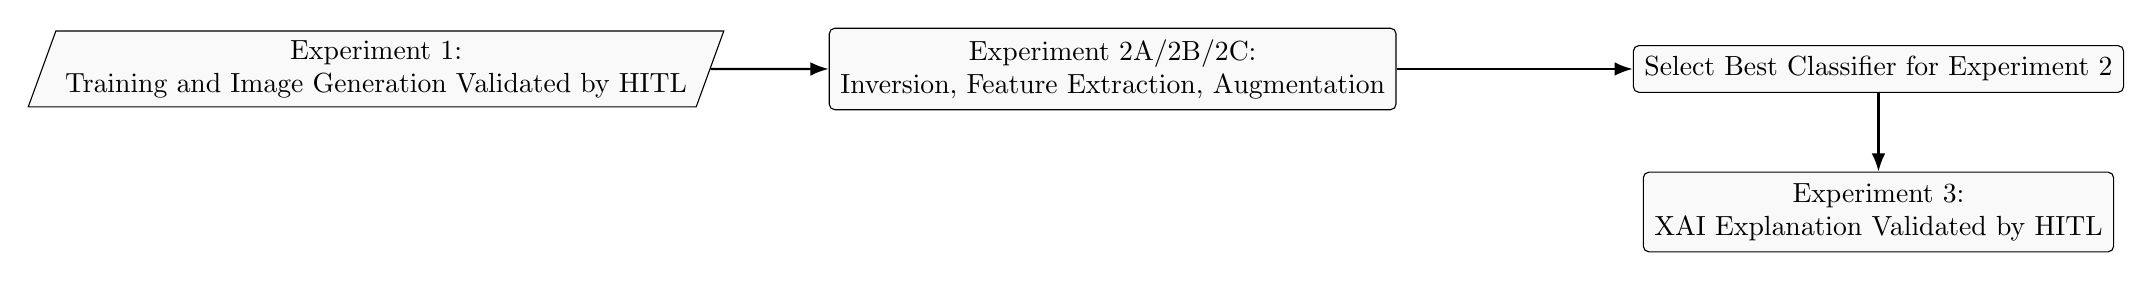
\begin{tikzpicture}[
  >=Latex,
  node distance=10mm and 15mm,
  box/.style={draw, rounded corners=2pt, fill=gray!5, align=center, minimum width=30mm, inner sep=4pt},
  io/.style={draw, trapezium, trapezium left angle=70, trapezium right angle=110, fill=gray!5, align=center, minimum width=34mm},
  decision/.style={diamond, draw, aspect=2, fill=gray!5, align=center, inner sep=1pt},
  line/.style={->, thick, rounded corners=2pt}
]

% Row 1 (Experiment 1)
\node[io]   (exp1)   {Experiment 1:\\ Training and Image Generation Validated by HITL};
\node[box, right=of exp1] (exp2) {Experiment 2A/2B/2C:\\Inversion, Feature Extraction, Augmentation};
\node[box, right=3 cm of exp2]  (select) {Select Best Classifier for Experiment 2};

% Row 2 (XAI)
\node[box, below=10mm of select] (xai) {Experiment 3:\\ XAI Explanation Validated by HITL};

% Arrows Row 1
\draw[line] (exp1) -- (exp2);
\draw[line] (exp2) -- (select);

% Arrows to Row 2 (XAI)
\draw[line] (select) -- (xai);

\end{tikzpicture}%
}
\caption{Experimental Pipeline Overview}
\label{fig:experiment_pipeline}
\end{figure}


\section{Overall System Architecture}

Figure~\ref{fig:overall_architecture} presents the overall architecture of the proposed framework, illustrating how the three main components --- generation, classification, and explainability --- are integrated into a unified pipeline under strict patient-level data leakage control.

\begin{figure}[H]
\centering
\resizebox{0.88\textwidth}{!}{%
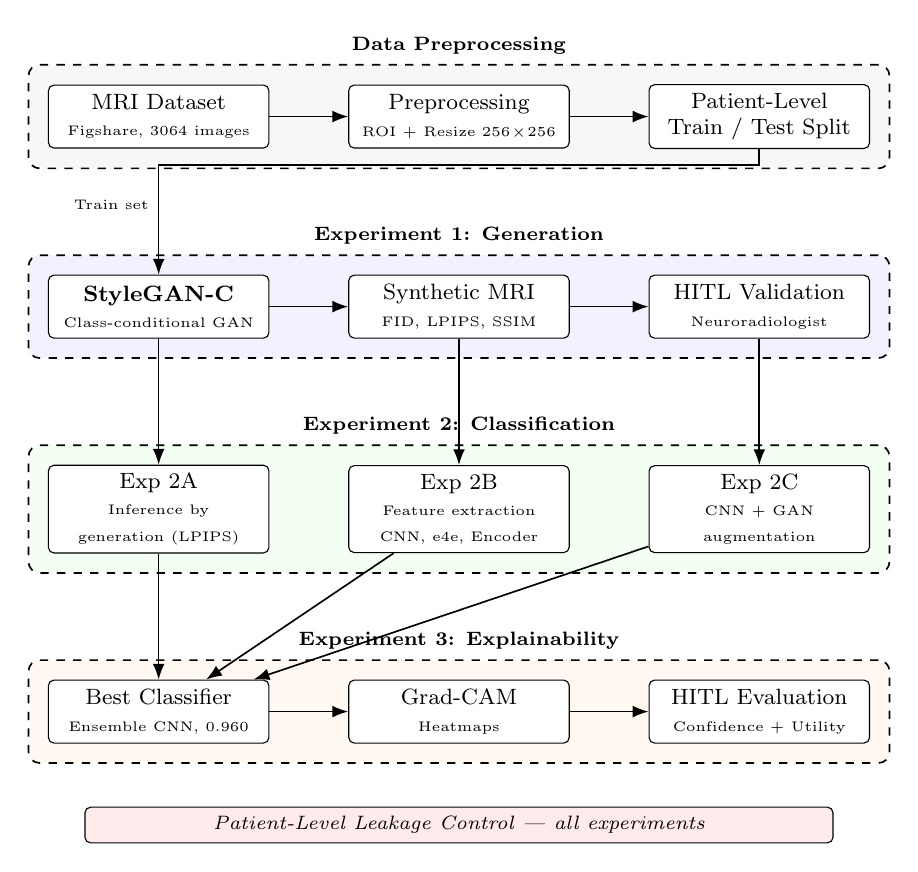
\begin{tikzpicture}[
  >=Latex,
  node distance=6mm and 10mm,
  box/.style={draw, rounded corners=2pt, fill=white, align=center, minimum width=28mm, minimum height=8mm, inner sep=3pt, font=\footnotesize},
  line/.style={->, semithick},
  gbox/.style={draw, dashed, rounded corners=4pt, inner sep=7pt, line width=0.6pt},
]

% === ROW 1: Data pipeline ===
\node[box] (data) {MRI Dataset\\{\tiny Figshare, 3064 images}};
\node[box, right=of data] (prep) {Preprocessing\\{\tiny ROI + Resize $256\!\times\!256$}};
\node[box, right=of prep] (split) {Patient-Level\\Train / Test Split};

\draw[line] (data) -- (prep);
\draw[line] (prep) -- (split);

% === ROW 2: Experiment 1 ===
\node[box, below=16mm of data] (gan) {\textbf{StyleGAN-C}\\{\tiny Class-conditional GAN}};
\node[box, right=of gan] (synth) {Synthetic MRI\\{\tiny FID, LPIPS, SSIM}};
\node[box, right=of synth] (hitl1) {HITL Validation\\{\tiny Neuroradiologist}};

\draw[line] (split.south) -- ++(0,-2mm) -| node[above left, font=\tiny, pos=0.75]{Train set} (gan.north);
\draw[line] (gan) -- (synth);
\draw[line] (synth) -- (hitl1);

% === ROW 3: Experiment 2 ===
\node[box, below=16mm of gan] (e2a) {Exp 2A\\{\tiny Inference by}\\{\tiny generation (LPIPS)}};
\node[box, right=of e2a] (e2b) {Exp 2B\\{\tiny Feature extraction}\\{\tiny CNN, e4e, Encoder}};
\node[box, right=of e2b] (e2c) {Exp 2C\\{\tiny CNN + GAN}\\{\tiny augmentation}};

\draw[line] (gan) -- (e2a);
\draw[line] (synth) -- (e2b);
\draw[line] (hitl1.south) -- ++(0,-2mm) -| (e2c.north);

% === ROW 4: Experiment 3 ===
\node[box, below=16mm of e2a] (best) {Best Classifier\\{\tiny Ensemble CNN, 0.960}};
\node[box, right=of best] (gradcam) {Grad-CAM\\{\tiny Heatmaps}};
\node[box, right=of gradcam] (hitl2) {HITL Evaluation\\{\tiny Confidence + Utility}};

\draw[line] (e2a) -- (best);
\draw[line] (e2b) -- (best);
\draw[line] (e2c) -- (best);
\draw[line] (best) -- (gradcam);
\draw[line] (gradcam) -- (hitl2);

% === GROUP BOXES ===
\begin{scope}[on background layer]
  \node[gbox, fill=gray!6, fit=(data)(prep)(split), label={[font=\scriptsize\bfseries]above:Data Preprocessing}] {};
  \node[gbox, fill=blue!5, fit=(gan)(synth)(hitl1), label={[font=\scriptsize\bfseries]above:Experiment 1: Generation}] {};
  \node[gbox, fill=green!5, fit=(e2a)(e2b)(e2c), label={[font=\scriptsize\bfseries]above:Experiment 2: Classification}] {};
  \node[gbox, fill=orange!5, fit=(best)(gradcam)(hitl2), label={[font=\scriptsize\bfseries]above:Experiment 3: Explainability}] {};
\end{scope}

% === Leakage bar ===
\node[draw, fill=red!8, rounded corners=2pt, font=\scriptsize\itshape, align=center, below=8mm of gradcam, minimum width=95mm] {Patient-Level Leakage Control --- all experiments};

\end{tikzpicture}%
}
\caption{Overall system architecture. The pipeline integrates data preprocessing, class-conditional generation (Experiment~1), multi-strategy classification (Experiment~2), and explainability with clinical validation (Experiment~3), all under strict patient-level data leakage control.}
\label{fig:overall_architecture}
\end{figure}

The implementation was developed using Python 3.12.12 within a Google Colab virtual machine running on Linux (x86\_64 architecture). The hardware configuration included an Intel Xeon CPU, 167\,GB of RAM, and an NVIDIA A100 GPU with 80\,GB of HBM memory, CUDA~12.x support, and AMP for mixed-precision training (fp16/fp32). Key libraries and frameworks used include \texttt{torch} 2.8.0+cu126 for deep learning, \texttt{torchvision}, the official NVLabs StyleGAN2-ADA (PyTorch) repository, and the LPIPS metric based on VGG. Additional utilities included \texttt{gdown} 5.2.0 for downloading assets, \texttt{numpy} 2.0.2 for numerical computations, \texttt{Pillow} 11.3.0 for image handling, \texttt{matplotlib} 3.10.0 for plotting, \texttt{ninja} 1.13.0 for build speedup, and \texttt{opensimplex} 0.4.5.1 for noise generation. Scikit-learn and scikit-image were also used for various preprocessing and evaluation tasks. GPU-based SSIM was computed using the \texttt{piq} package. Core Python modules such as \texttt{os}, \texttt{shutil}, \texttt{pathlib}, and \texttt{subprocess} were used extensively, although these are standard library modules and do not expose a \texttt{\_\_version\_\_} attribute. The \texttt{legacy} module employed for loading models is included as part of the StyleGAN2-ADA codebase and does not have a separate version identifier.
During the preparation of this thesis, the default Google Colab libraries were updated by Google. 
All experiments reported in this thesis were executed using the Colab environment as available in October~2025. For reproducibility, it is recommended to run the provided notebooks with package versions matching this October~2025 configuration.



\section{Dataset Description}

\begin{itemize}
  
    \item \textbf{Figshare Dataset:} This T1-weighted contrast-enhanced magnetic resonance dataset was acquired after Gd-DTPA injection from two hospitals in China: Nanfang Hospital, Guangzhou, and General Hospital, Tianjin Medical University, between September 2005 and October 2010. All images were obtained using a contrast dose of 0.1 mmol/kg Gd-DTPA administered at a rate of 2 ml/s. The scans have an in-plane resolution of $512 \times 512$ with pixel dimensions of $0.49 \times 0.49\,\text{mm}^2$, a slice thickness of 6 mm, and a slice gap of 1 mm. The dataset contains 3,064 images from 233 patients, distributed across three tumor types: \textit{meningioma} (708 images), \textit{glioma} (1,426 images), and \textit{pituitary} (930 images). It includes three standard anatomical views: axial, coronal, and sagittal~\cite{cheng2017figshare} \cite{Cheng2015}.\\
    \end{itemize}

By design, no patient appeared in both partitions (training and testing), ensuring that test performance genuinely reflected generalization to unseen subjects, rather than to new slices from patients already seen during training. As shown in Table~\ref{tab:dataset_all_one}, in addition to the full dataset, a reduced variant of the dataset was constructed by excluding MRI slices of poor diagnostic quality (e.g., slices with minimal tumor visibility or significant artifacts). This reduced dataset excludes 761 images, corresponding to approximately 25\% fewer images than the complete dataset. Both variants preserve patient-level leakage control in their train--test partitions.

\begin{table}[ht]
\centering
\caption{Dataset summary Original vs.\ Reduced splits (Train/Test).}
\label{tab:dataset_all_one}
\setlength{\tabcolsep}{5pt}
\begin{tabular}{lcccccccc}
\toprule
 & \multicolumn{2}{c}{Train (Original)} & \multicolumn{2}{c}{Test (Original)} & \multicolumn{2}{c}{Train (Reduced)} & \multicolumn{2}{c}{Test (Reduced)} \\
\cmidrule(lr){2-3}\cmidrule(lr){4-5}\cmidrule(lr){6-7}\cmidrule(lr){8-9}
Class & Images & Patients & Images & Patients & Images & Patients & Images & Patients \\
\midrule
Glioma     & 980 & 59 & 446 & 30 & 634 & 54 & 312 & 29 \\
Meningioma & 514 & 60 & 194 & 22 & 406 & 58 & 141 & 21 \\
Pituitary  & 659 & 44 & 271 & 18 & 561 & 44 & 249 & 18 \\
\midrule
\textbf{Total} & \textbf{2153} & \textbf{163} & \textbf{911} & \textbf{70} & \textbf{1601} & \textbf{156} & \textbf{702} & \textbf{68} \\
\bottomrule
\end{tabular}
\end{table}

\newpage
\subsection{Image Preprocessing}
The preprocessing pipeline applied to the MRI images comprises a sequence of carefully designed steps.
\begin{enumerate}
    \item \textbf{Image Loading and Labelling:} \\
    Each image file is read into memory and assigned its tumor class label (glioma, meningioma, pituitary) together with a patient identifier taken from the original dataset structure. Files that cannot be loaded are skipped to maintain data integrity.

    \item \textbf{Automatic Region of Interest (ROI) Extraction:}
    \begin{itemize}
        \item \textit{Grayscale Conversion:} The RGB image is converted to grayscale, reducing it from three channels to one. This simplifies subsequent processing, as most MRI scans are inherently grayscale.
        \item \textit{Gaussian Blurring:} A Gaussian filter with a $3 \times 3$ kernel is applied to smooth the image and suppress high frequency noise.
        \item \textit{Thresholding:} The blurred image is binarized using a fixed intensity.
        \item \textit{Morphological Operations:} Erosion is applied to eliminate small noise regions, followed by dilation to restore the main object's size and fill small holes.
        \item \textit{Contour Detection and Selection:} External contours in the binary mask are detected. The largest contour by area is selected, which is assumed to correspond to the main anatomical structure, such as the brain.
        \item \textit{Bounding Box Determination:} The extreme points of the selected contour define a minimal bounding rectangle that encloses the ROI.
        \item \textit{Image Cropping:} The original image is cropped to this bounding box, resulting in an image focused on the region of interest with minimal background.
    \end{itemize}

    \item \textbf{Resizing to Fixed Dimensions:} \\
    The ROI is resized to a fixed square resolution $256 \times 256$ pixels. This sampling step standardizes input sizes for CNNs, reduces memory usage, and ensures batch compatibility.

    \item \textbf{Saving the Processed Images:} \\
    Processed images are saved in a new output directory using a uniform image format (PNG). This prepares the dataset for efficient loading during model training and evaluation.

\end{enumerate}


\subsection{Patient-wise data splits and leakage control}
\label{subsec:patient_splits}

\paragraph{Patient-wise partitioning.}
Patient identifiers (PIDs) are first extracted from all preprocessed MRI slices, and all splits are defined at the patient level to avoid information leakage across training and testing. The full set of patients is then partitioned into:
\begin{itemize}
    \item a training patient set $\mathcal{G}_{\text{train}}$ (70\% of the patients),
    \item a test patient set $\mathcal{G}_{\text{test}}$ (30\% of the patients),
\end{itemize}
such that
\[
\mathcal{G}_{\text{train}} \cap \mathcal{G}_{\text{test}} = \emptyset.
\]

All slices from patients in $\mathcal{G}_{\text{train}}$ are used exclusively for training, and all slices from patients in $\mathcal{G}_{\text{test}}$ are used exclusively for testing. This guarantees that no patient, and thus no slice from the same patient, appears in both the training and test sets.

\paragraph{Leakage control and reproducibility.}
Across all experiments, data leakage is controlled through a combination of structural constraints and implementation checks:
\begin{itemize}
    \item there is no overlap of patient identifiers between the training and test groups.
    \item synthetic images used in augmentation and generation based classification experiments are generated only from real images belonging to patients in $\mathcal{G}_{\text{train}}$.
\end{itemize}



\begin{figure}[H]
    \centering
    
\includegraphics[width=0.9\textwidth]{Template-Tesis-dii/img/secuence.png} % Sustituye "tu_imagen.jpg" con el nombre de tu archivo
    \caption{Six similar sequences of glioma from the same patient.}
    \label{fig:sequences}
\end{figure}

Multiple MRI sequences from the same patient can contain nearly identical slices. When these slices are split across training and testing sets, they introduce data leakage and risk overfitting, as the model may memorize patient-specific details.

\newpage

\section{Experiment 1: Image Generation}



\begin{figure}[h]
\centering
\resizebox{1\linewidth}{!}{%
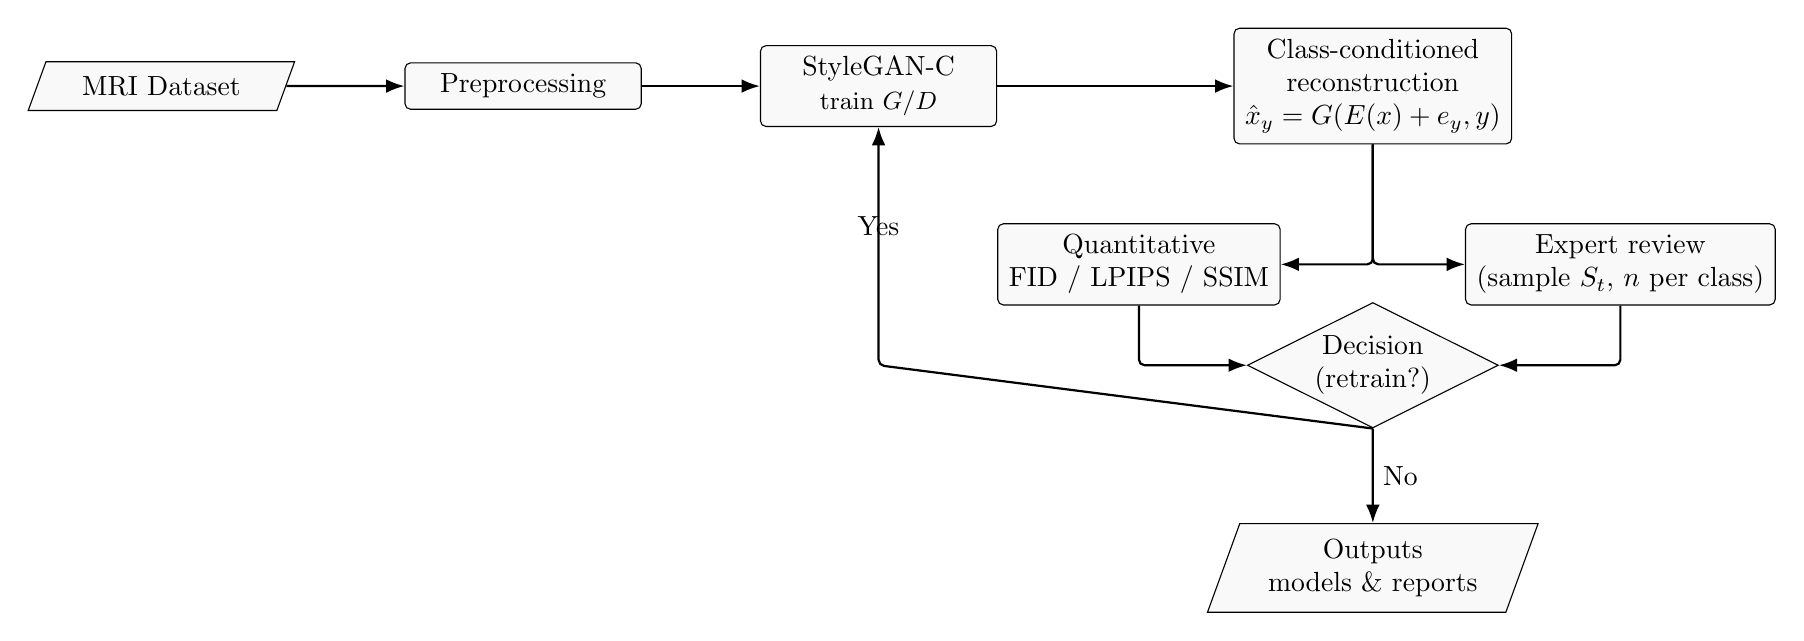
\begin{tikzpicture}[
  >=Latex,
  node distance=10mm and 15mm,
  box/.style={draw, rounded corners=2pt, fill=gray!5, align=center, minimum width=30mm, inner sep=4pt},
  io/.style={draw, trapezium, trapezium left angle=70, trapezium right angle=110, fill=gray!5, align=center, minimum width=34mm},
  decision/.style={diamond, draw, aspect=2, fill=gray!5, align=center, inner sep=1pt},
  line/.style={->, thick, rounded corners=2pt}
]

% Row 1 (left to right)
\node[io]   (data)   {MRI Dataset};
\node[box, right=of data] (prep) {Preprocessing};
\node[box, right=of prep] (gan)  {StyleGAN-C\\\small train $G/D$};
\node[box, right=3 cm of gan]  (reco) {Class-conditioned\\reconstruction\\$\hat{x}_y = G(E(x)+e_y,y)$};

% Evaluation branches
\node[box, below left=10mm and -6mm of reco] (quant) {Quantitative\\FID / LPIPS / SSIM};
\node[box, below right=10mm and -6mm of reco] (clin) {Expert review\\(sample $S_t$, $n$ per class)};

% Decision
\node[decision, below=20mm of reco] (dec) {Decision\\(retrain?)};

% Outputs directly under decision
\node[io, below=12mm of dec, minimum width=42mm] (out) {Outputs\\models \& reports};

% Arrows row 1
\draw[line] (data) -- (prep);
\draw[line] (prep) -- (gan);
\draw[line] (gan) -- (reco);

\draw[line] (reco) |- (quant);
\draw[line] (reco) |- (clin);

\draw[line] (quant) |- (dec);
\draw[line] (clin)  |- (dec);

% No -> straight down to outputs
\draw[line] (dec) -- node[right]{No} (out);

% Yes -> explicit clean L (no triangle)
\draw[line] (dec.south) -- (dec.west -| gan.south)
           -- node[pos=0.5, above]{Yes} (gan.south);

\end{tikzpicture}%
}
\caption{Experiment 1 Image Generation Pipeline.}
\label{fig:exp1_pipeline}
\end{figure}


\subsection{Conditional StyleGAN2-ADA Architecture}
\label{subsec:stylegan_arch}
In this thesis, \textbf{StyleGAN-C} denotes a lightly modified conditional version of StyleGAN2-ADA \cite{Karras2019stylegan2}, adapted to brain tumor MRI synthesis with minimal architectural changes. A target resolution of $256\times256$ pixels was selected as it strikes a balance between performance and computational efficiency. Higher resolutions (e.g., $512\times512$) could capture finer anatomical detail but at significantly higher computational cost, while lower resolutions (e.g., $128\times128$) would reduce demands but risk losing diagnostically relevant information. \\

The generator extends StyleGAN2-ADA with explicit class conditioning. A latent vector \(z \sim \mathcal{N}(0, I)\) is mapped by the mapping network to a disentangled code \(w = f(z)\), while each discrete label \(y \in \mathcal{Y}\) is embedded via a learnable layer \(E(y) = e_y \in \mathbb{R}^d\). To steer synthesis toward class specific distributions, the model fuses class and style in \(\mathcal{W}\) using an additive rule \(w^\star = w + A e_y\) with a learnable projection \(A\). The synthesis network \(G(\cdot, y)\) then applies per layer style modulation (AdaIN) driven by affine transforms of \(w^\star\) , yielding class controlled images \(\hat{x}_y = G(w^\star, y)\). 
\\

For brain MRI, the original implementation is adapted to operate on \textbf{single-channel} grayscale images, so the generator outputs one channel and the discriminator input stem accepts tensors of shape \(1 \times H \times W\). Operationally, sampling proceeds as
\(z \rightarrow w \rightarrow w^\star = w + A e_y \rightarrow \hat{x}_y = G(w^\star, y)\), with truncation in \(\mathcal{W}\) to control sample typicality.


\subsection{Training}

A patient-level split of 70\%-30\% was applied to create the training and testing partitions, respectively, ensuring that no patient appears in both splits and thus preventing data leakage in subsequent experiments; only the training set was used to fit the conditional GAN. Class conditionality was enabled by organizing images into class specific folders and building a filename class index mapping consumed by the dataset loader. The single channel (grayscale) StyleGAN-C was trained with StyleGAN2-ADA using the following hyperparameters: \texttt{\string--cfg=24gb-gpu}, \texttt{\string--gpus=1}, \texttt{\string--batch=32}, \texttt{\string--cond=1}, \texttt{\string--aug=ada}, \texttt{\string--target=0.6}, \texttt{\string--augpipe=bg}, \texttt{\string--mirror=1}, \texttt{\string--snap=50}, \texttt{\string--workers=12}, \texttt{\string--metrics=none}, \texttt{\string--kimg=1000}.


\subsection{Image Generation}

For image synthesis, the repository’s generation utility is used to initialize the trained generator at a selected network snapshot. Under class conditional operation, a designated class identifier guides the synthesis toward the corresponding semantic manifold, while optional truncation in the \(\mathcal{W}\) space modulates sample typicality. The utility produces seed-controlled outputs.


\subsection{Class-Conditioned Image Generation by Reconstruction}
\label{subsec:generation_reconstruction}

\begin{figure}[ht]
\centering
\resizebox{1\textwidth}{!}{%
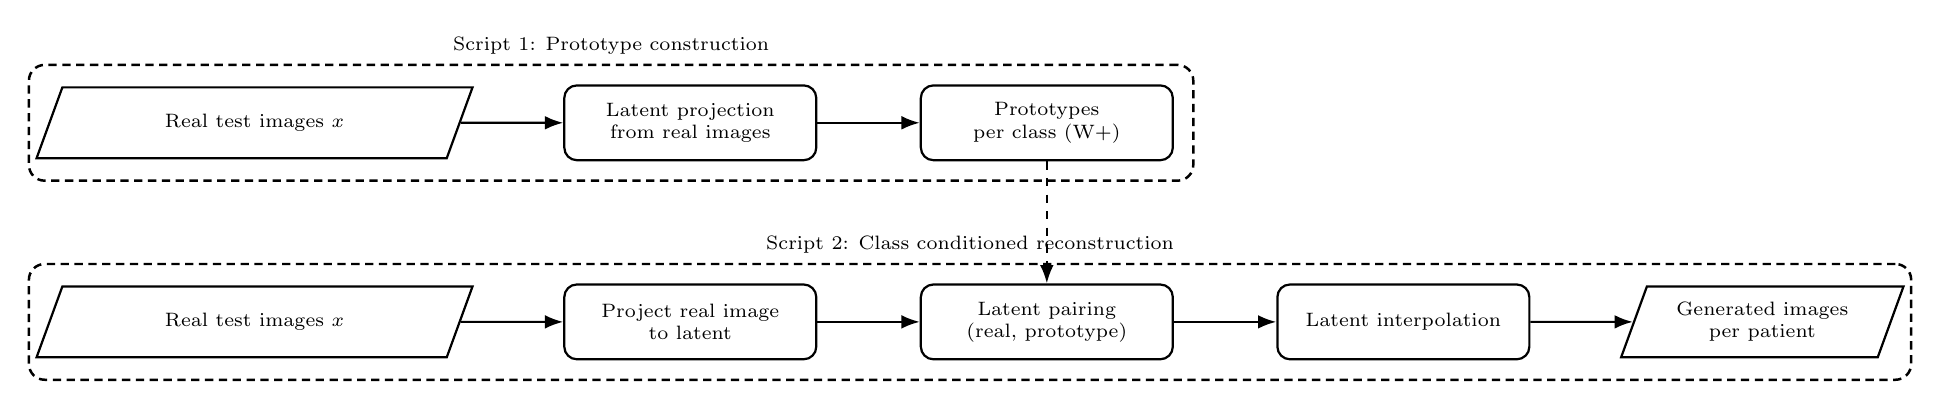
\begin{tikzpicture}[node distance=1.0cm and 1.3cm, >=Latex]

\tikzset{
  block/.style={
    rectangle, rounded corners=1.6mm,
    draw, thick, align=center,
    minimum height=0.95cm, minimum width=3.2cm,
    inner sep=3.5pt, font=\scriptsize
  },
  io/.style={
    trapezium, trapezium left angle=70, trapezium right angle=110,
    draw, thick, align=center,
    minimum height=0.9cm, minimum width=3.2cm,
    inner sep=3.5pt, font=\scriptsize
  },
  arrow/.style={->, thick},
  dashedarrow/.style={->, thick, dashed},
  dframe/.style={
    draw=black, line width=0.9pt, densely dashed,
    rounded corners=2mm, inner sep=7pt
  }
}

% ==========================
% Script 1 (top row)
% ==========================
\node[io] (ds) {Real test images $x$};
\node[block, right=of ds] (proj) {Latent projection\\from real images};
\node[block, right=of proj] (proto) {Prototypes\\per class (W+)};

\draw[arrow] (ds) -- (proj);
\draw[arrow] (proj) -- (proto);

% ==========================
% Script 2 (bottom row)
% ==========================
\node[io, below=1.6cm of ds] (x2) {Real test images $x$};
\node[block, right=of x2] (wreal) {Project real image\\to latent};
\node[block, right=of wreal] (pair) {Latent pairing\\(real, prototype)};
\node[block, right=of pair] (interp) {Latent interpolation};
\node[io, right=of interp] (cfset) {Generated images\\per patient};

\draw[arrow] (x2) -- (wreal);
\draw[arrow] (wreal) -- (pair);
\draw[arrow] (pair) -- (interp);
\draw[arrow] (interp) -- (cfset);

% Cross-script dependency
\draw[dashedarrow] (proto.south) to[out=-90, in=90, looseness=0.9] (pair.north);

% ==========================
% Dotted frames (background)
% ==========================
\begin{scope}[on background layer]
  \node[dframe, fit=(ds)(proj)(proto)] (frame1) {};
  \node[dframe, fit=(x2)(wreal)(pair)(interp)(cfset)] (frame2) {};
\end{scope}

% Titles for frames
\node[font=\scriptsize, anchor=south] at (frame1.north) {Script 1: Prototype construction};
\node[font=\scriptsize, anchor=south] at (frame2.north) {Script 2: Class conditioned reconstruction};

\end{tikzpicture}%
}
\caption{Experiment 1 (Part 2): two scripts. Script 1 computes latent prototypes per class from real images. Script 2 reconstructs each real test image by interpolating its latent code toward each class prototype.}
\label{fig:exp1_part2_two_scripts}
\end{figure}



Class conditioned images are generated through a prototype based reconstruction process that starts from real MRI slices and produces sets of class specific counterfactuals. First, for each tumor class \(c \in \mathcal{C}\), a latent prototype \(\mu_c \in \mathcal{W}^+\) is estimated by projecting multiple training images of that class with the StyleGAN2-ADA \cite{Karras2019stylegan2} projector and averaging their final inverted codes. Given an input image \(x\) from the test set, an inversion module \(P(\cdot)\) maps \(x\) into the latent space of the StyleGAN-C generator, yielding a patient specific code \(w_{\text{real}} = P(x)\). For each target class \(c \in \mathcal{C}\), a two point latent pair \((w_{\text{real}}, \mu_c)\) is then used to define an interpolation trajectory in \(\mathcal{W}^+\). \\

Iterating over all classes and interpolation steps produces one trajectory that remains close to the original class and additional counterfactual trajectories that move towards alternative class prototypes, enabling controlled class wise variation while preserving patient specific structure.


\subsection{Evaluation Protocol}
\label{subsec:evaluation_protocol}

\paragraph{Quantitative Evaluation.}
To assess the quality of generated images, the thesis employs the following metrics:
\begin{itemize}
    \item \textbf{FID (Fréchet Inception Distance):} measuring distributional similarity between real and generated images.
    \item \textbf{LPIPS (Learned Perceptual Image Patch Similarity):} evaluating perceptual similarity with respect to the input.
    \item \textbf{SSIM (Structural Similarity Index):} assessing structural fidelity relevant to anatomical integrity.
    \item \textbf{PSNR (Peak Signal-to-Noise Ratio):} a reconstruction metric that compares each generated image to its real reference at the pixel level; higher PSNR indicates lower distortion and therefore closer agreement between synthetic and real images.
\end{itemize}

FID is computed at the set level by comparing the distribution of real images against the distribution of generated images within each class. In contrast, LPIPS, SSIM, and PSNR are evaluated in a pairwise manner only in the reconstruction setting.


\paragraph{Qualitative Evaluation (Clinical).}
One neuroradiologist performed a blinded qualitative evaluation of a set of \(N\) real and generated MR images. This experiment is designed as a pilot feasibility study with a single evaluator, intended to provide initial evidence on the clinical plausibility of synthetic images and the utility of XAI overlays. The sample size ($n=33$ images) limits statistical power but establishes a protocol for future multi-reader studies. The expert was asked to:
\begin{enumerate}
    \item Rate the \textbf{diagnostic confidence and perceived clinical utility} of each image using a 1--5 Likert scale.
    \item Judge whether each generated image is \textbf{consistent with its assigned tumor class}.
\end{enumerate}




\newpage

\section{Experiment 2: Classification Models Integrating StyleGAN-C}
\label{sec:exp2_overview}

Experiment~2 investigates how to best integrate the conditional StyleGAN-C generator into the brain tumor classification pipeline. The main goal is to explore different classification strategies that exploit the generator, either through latent inversion and counterfactual synthesis or through synthetic data augmentation, and to identify the most effective approach. To this end, three complementary subexperiments are defined.\\

Experiment~2A studies \emph{optimization based latent inversion}. For each real MRI slice, a latent code in the StyleGAN-C $W^+$ space is obtained by running the projector, and class specific prototypes are estimated by averaging multiple projected codes per class. These latent representations are then used to generate class conditional trajectories, which support two classifiers: (i) a generation based classifier that assigns the label by minimizing LPIPS distance between the real slice and its class conditioned reconstructions, and (ii) a CNN that observes only the generated counterfactual images and aggregates slice level probabilities at the patient level.\\

Experiment~2B focuses on \emph{encoder based latent inversion}. Three families of slice level features are considered: (i) convolutional features from a fine tuned ResNet-50 tumor classifier; (ii) latent codes produced by a supervised encoder that maps MRI slices into the latent space; and (iii) latent codes obtained from an e4e encoder, initially pre trained on FFHQ and fine tuned on the brain tumor dataset. Each representation is evaluated independently as input to a linear SVM, in order to assess whether StyleGAN-C latent embeddings provide complementary information to standard convolutional features.\\


Experiment~2C evaluates \emph{StyleGAN-C as a data augmentation engine}. Here, the generator is trained only on the training split, and synthetic images are sampled to balance under represented tumor classes. A ResNet-50 ensemble is then trained under two conditions: a real only baseline and a GAN balanced configuration where synthetic MRIs are added until matching the majority class. In addition, controlled leakage scenarios are analyzed to quantify how training the generator on non-disjoint patient splits can artificially inflate test performance, highlighting the importance of strict patient-level separation in all augmentation experiments.\\


Across these three subexperiments, the different configurations are compared primarily in terms of macro-averaged F1-score and overall accuracy on the test set. The most promising model is selected as the final tumor classification strategy adopted in this thesis.


\newpage

\section{Experiment 2A: Inference By Generation}
\label{subsec:gated_ensemble_lpips_simple}


\begin{figure}[H]
\centering
\resizebox{0.85\textwidth}{!}{%
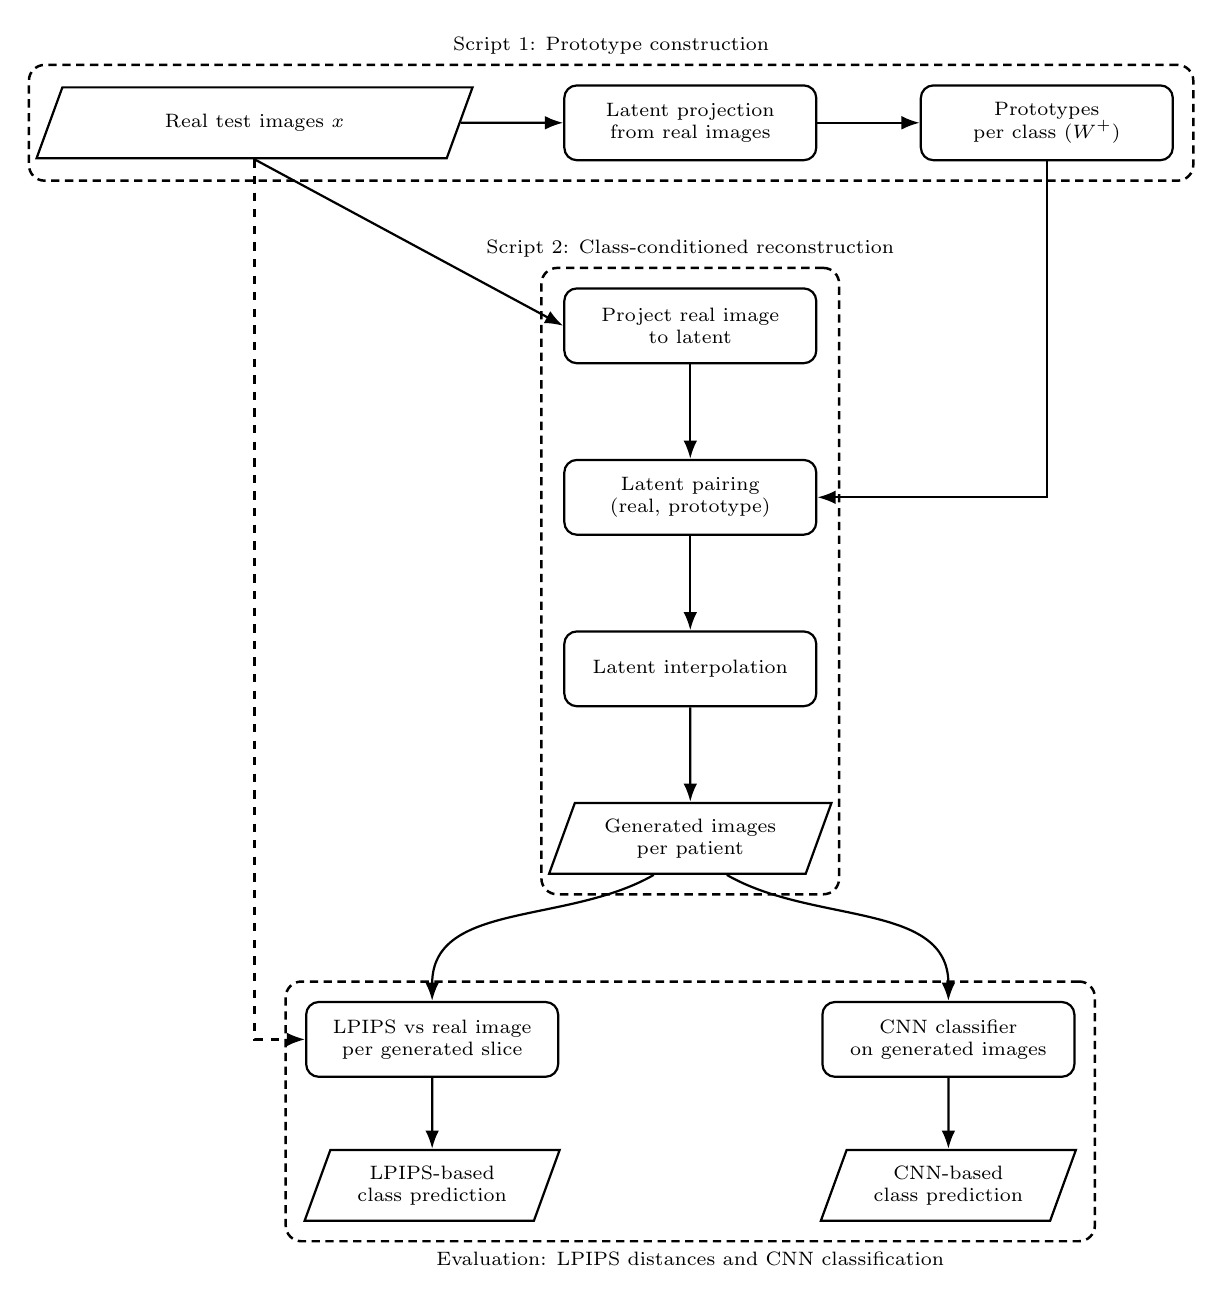
\begin{tikzpicture}[node distance=1.0cm and 1.3cm, >=Latex]

\tikzset{
  block/.style={
    rectangle, rounded corners=1.6mm,
    draw, thick, align=center,
    minimum height=0.95cm, minimum width=3.2cm,
    inner sep=3.5pt, font=\scriptsize
  },
  io/.style={
    trapezium, trapezium left angle=70, trapezium right angle=110,
    draw, thick, align=center,
    minimum height=0.9cm, minimum width=3.2cm,
    inner sep=3.5pt, font=\scriptsize
  },
  arrow/.style={->, thick},
  dashedarrow/.style={->, thick, dashed},
  dframe/.style={
    draw=black, line width=0.9pt, densely dashed,
    rounded corners=2mm, inner sep=7pt
  }
}

% ==========================
% Script 1 (fila superior)
% ==========================
\node[io] (ds) {Real test images $x$};
\node[block, right=of ds] (proj) {Latent projection\\from real images};
\node[block, right=of proj] (proto) {Prototypes\\per class ($W^+$)};

\draw[arrow] (ds) -- (proj);
\draw[arrow] (proj) -- (proto);

% ==========================
% Script 2 (columna central, centrada bajo proj)
% ==========================
\node[block, below=1.6cm of proj] (wreal) {Project real image\\to latent};
\node[block, below=1.2cm of wreal] (pair) {Latent pairing\\(real, prototype)};
\node[block, below=1.2cm of pair] (interp) {Latent interpolation};
\node[io,    below=1.2cm of interp] (cfset) {Generated images\\per patient};

% Conexión desde las imágenes reales (script 1) al script 2
\draw[arrow] (ds.south) -- (wreal.west);

\draw[arrow] (wreal) -- (pair);
\draw[arrow] (pair) -- (interp);
\draw[arrow] (interp) -- (cfset);

% Dependencia entre scripts (prototipos -> pairing) en forma de L
\draw[arrow] (proto.south) |- (pair.east);

% ==========================
% Rama de evaluación (debajo de cfset)
% ==========================

% LPIPS (izquierda)
\node[block, below left=1.6cm and 1.2cm of cfset] (lpips) {LPIPS vs real image\\per generated slice};
\node[io, below=0.9cm of lpips] (lpips_pred) {LPIPS-based\\class prediction};

\draw[arrow] (cfset.south west) to[out=-150, in=90] (lpips.north);
\draw[arrow] (lpips) -- (lpips_pred);

% NUEVA LÍNEA: real test images -> LPIPS (para indicar la referencia real)
\draw[dashedarrow] (ds.south) |- (lpips.west);

% CNN (derecha)
\node[block, below right=1.6cm and 1.2cm of cfset] (cnn_cf) {CNN classifier\\on generated images};
\node[io, below=0.9cm of cnn_cf] (cnn_pred) {CNN-based\\class prediction};

\draw[arrow] (cfset.south east) to[out=-30, in=90] (cnn_cf.north);
\draw[arrow] (cnn_cf) -- (cnn_pred);

% ==========================
% Marcos punteados
% ==========================
\begin{scope}[on background layer]
  \node[dframe, fit=(ds)(proj)(proto)] (frame1) {};
  \node[dframe, fit=(wreal)(pair)(interp)(cfset)] (frame2) {};
  \node[dframe, fit=(lpips)(lpips_pred)(cnn_cf)(cnn_pred)] (frame3) {};
\end{scope}

% Títulos de los marcos
\node[font=\scriptsize, anchor=south] at (frame1.north) {Script 1: Prototype construction};
\node[font=\scriptsize, anchor=south] at (frame2.north) {Script 2: Class-conditioned reconstruction};
\node[font=\scriptsize, anchor=north] at (frame3.south) {Evaluation: LPIPS distances and CNN classification};

\end{tikzpicture}%
}
\caption{Experiment~1 (Part~2): prototype construction (top), class-conditioned reconstruction (middle), and evaluation (bottom). The evaluation stage includes two branches: LPIPS-based comparison between each generated image and its real counterpart, and CNN-based classification over the generated images per patient.}
\label{fig:exp1_part2_two_scripts_extended}
\end{figure}


\subsection{CNN classifier on generated counterfactuals}
\label{subsec:cnn_counterfactuals}

The CNN component is based on a ResNet-50 architecture whose final fully connected layer is adapted to the three tumor classes. The network is first trained on real MRI slices under the reduced dataset configuration described in Experiment~2C (truncation $\psi = 1.3$), and the resulting checkpoint is reused as a frozen classifier in the present experiment.

At inference time, the classifier operates on StyleGAN-C counterfactuals. For each patient, the method receives a set of class conditioned generated images produced by the latent interpolation procedure. The ResNet-50, which outputs a class-probability vector
\[
\mathbf{p}^{\text{cnn}}_{p,c,f} \in \mathbb{R}^C
\]
for the slice associated with patient $p$, target class $c$ and frame index $f$.

To obtain a patient level prediction, slice level probabilities are combined using predefined frame and class weights. Let $w^{\text{frame}}_f$ denote the weight associated with frame $f$ along the counterfactual trajectory and $w^{\text{class}}_c$ the weight associated with target class $c$. The total weight for a generated slice is defined as
\[
w_{c,f} = w^{\text{class}}_c \, w^{\text{frame}}_f,
\]
and the aggregated CNN probability vector for patient $p$ is given by
\[
\bar{\mathbf{p}}^{\text{cnn}}_p
=
\frac{1}{Z_p}
\sum_{c=1}^{C}
\sum_{f} w_{c,f} \, \mathbf{p}^{\text{cnn}}_{p,c,f},
\qquad
Z_p = \sum_{c=1}^{C} \sum_{f} w_{c,f}.
\]
The CNN-based patient level prediction is then obtained by
\[
\hat{y}^{\text{cnn}}_p = \arg\max_{c} \bar{p}^{\text{cnn}}_{p,c},
\]
providing a purely discriminative baseline that operates exclusively on the generated counterfactual images.




\subsection{LPIPS inference by generation.}

In parallel, the framework performs inference by generation using LPIPS as a perceptual similarity measure. For each real slice of a patient and each class, the method computes the LPIPS distance between the real image and its corresponding class conditional reconstruction. These distances are aggregated per class and per patient into a vector where smaller values indicate better reconstructions for that class.\\

Because LPIPS distances are not probabilities and live on a small numeric range, they are converted into a probability distribution in two steps: (i) a per-patient min-max normalization is applied to map distances to $[0,1]$, and (ii) a temperature-scaled softmax is applied over the negated distances:
\[
\bar{\mathbf{p}}^{\text{lpips}}_p
=
\text{softmax}\!\left(- \frac{\mathbf{D}'_p}{T_{\text{lpips}}}\right),
\]
where $\mathbf{D}'_p$ is the normalized distance vector and $T_{\text{lpips}}>0$ is a temperature hyperparameter controlling how peaked the distribution is. The LPIPS prediction is then given by
\[
\hat{y}^{\text{lpips}}_p = \arg\max_{c} \bar{p}^{\text{lpips}}_{p,c}.
\]

\subsubsection{Class-conditional counterfactual videos as visual explanations}

In addition to the quantitative evaluation based on CNN predictions, the proposed pipeline also produces class conditional counterfactual \emph{videos} that can be inspected by human experts as an explainability artefact. For each test patient, a representative MRI slice is first projected into the latent space of the StyleGAN-C generator, obtaining a latent code $\mathbf{w}_{\text{real}}$. Then, for every tumor class $y \in \{\text{glioma}, \text{meningioma}, \text{pituitary}\}$, a pair $(\mathbf{w}_{\text{real}}, \mathbf{w}_{\text{proto}}^{(y)})$ is constructed and a smooth interpolation in latent space is generated between the real code and the corresponding class prototype $\mathbf{w}_{\text{proto}}^{(y)}$. Each interpolation is rendered as a short video, with one frame per latent step.\\

These videos show how the image would gradually deform if it were forced to move towards each tumor class manifold according to the generator. From an XAI perspective, this provides an intuitive and clinically meaningful way to inspect the model's implicit representation of each class, turning the generative model into an interactive explanation tool rather than a purely black-box augmentation mechanism.

\clearpage


\section{Experiment 2B: Encoder based Latent Inversion}
\label{sec:exp2B_method}

\begin{figure}[ht]
\centering
\resizebox{1\textwidth}{!}{%
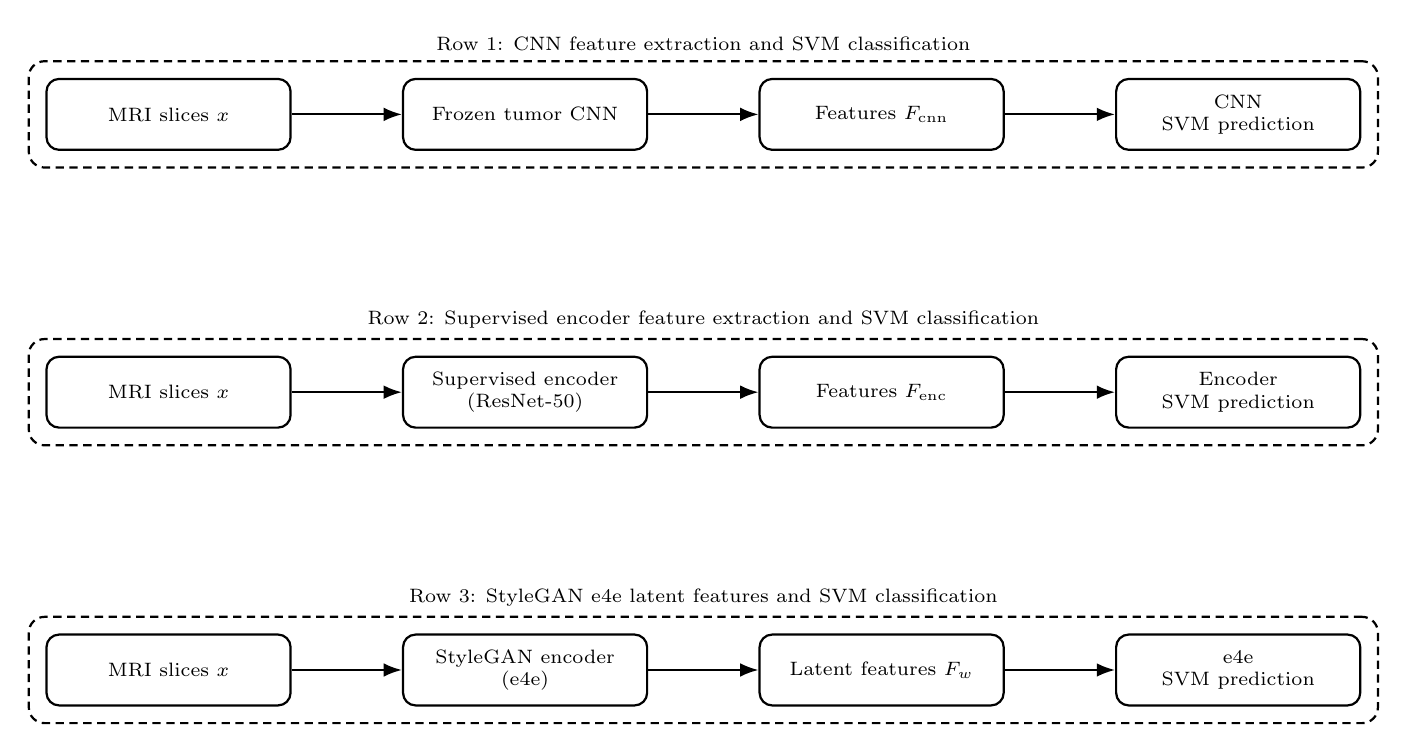
\begin{tikzpicture}[node distance=1.0cm and 1.4cm, >=Latex]

\tikzset{
  block/.style={
    rectangle, rounded corners=1.6mm,
    draw, thick, align=center,
    minimum height=0.9cm, minimum width=3.1cm,
    inner sep=3pt, font=\scriptsize
  },
  arrow/.style={->, thick},
  dashedarrow/.style={->, thick, dashed},
  dframe/.style={draw, thick, densely dashed, rounded corners=2mm, inner sep=6pt}
}

% =========================================================
% Row 1: CNN feature extraction -> classification
% =========================================================
\node[block] (x1)   {MRI slices $x$};
\node[block, right=of x1] (cnn)  {Frozen tumor CNN};
\node[block, right=of cnn] (fcnn) {Features $F_{\mathrm{cnn}}$};
\node[block, right=of fcnn] (ycnn) {CNN\\SVM prediction};

\draw[arrow] (x1) -- (cnn);
\draw[arrow] (cnn) -- (fcnn);
\draw[arrow] (fcnn) -- (ycnn);

% =========================================================
% Row 2: Supervised encoder -> classification
% =========================================================
\node[block, below=2.6cm of x1] (x3)   {MRI slices $x$};
\node[block, right=of x3] (enc)  {Supervised encoder\\(ResNet-50)};
\node[block, right=of enc] (fenc) {Features $F_{\mathrm{enc}}$};
\node[block, right=of fenc] (yenc) {Encoder\\SVM prediction};

\draw[arrow] (x3) -- (enc);
\draw[arrow] (enc) -- (fenc);
\draw[arrow] (fenc) -- (yenc);

% =========================================================
% Row 3: e4e encoder -> classification
% =========================================================
\node[block, below=2.6cm of x3] (x4)   {MRI slices $x$};
\node[block, right=of x4] (e4e)  {StyleGAN encoder\\(e4e)};
\node[block, right=of e4e] (fw) {Latent features $F_{w}$};
\node[block, right=of fw] (yw) {e4e\\SVM prediction};

\draw[arrow] (x4) -- (e4e);
\draw[arrow] (e4e) -- (fw);
\draw[arrow] (fw) -- (yw);

% =========================================================
% Dotted frames + labels
% =========================================================
\begin{scope}[on background layer]
  \node[dframe, fit=(x1)(cnn)(fcnn)(ycnn)] (frameCNN) {};
  \node[dframe, fit=(x3)(enc)(fenc)(yenc)] (frameENC) {};
  \node[dframe, fit=(x4)(e4e)(fw)(yw)] (frameE4E) {};
\end{scope}

\node[font=\scriptsize, anchor=south] at (frameCNN.north)
{Row 1: CNN feature extraction and SVM classification};
\node[font=\scriptsize, anchor=south] at (frameENC.north)
{Row 2: Supervised encoder feature extraction and SVM classification};
\node[font=\scriptsize, anchor=south] at (frameE4E.north)
{Row 3: StyleGAN e4e latent features and SVM classification};

\end{tikzpicture}%
}
\caption{Experiment~2B: comparison between CNN-based features, supervised encoder features, and StyleGAN e4e latent features, each evaluated with a linear SVM.}
\label{fig:exp2b_two_rows_cnn_encoder}
\end{figure}


The objective of this experiment is to investigate whether extracting deep features from a pre trained encoder with StyleGAN enables accurate classification. To this end, three configurations are compared:

\begin{enumerate}
    \item \textbf{CNN deep features}: A shallow classifier trained on deep features extracted from a tumor CNN (ResNet-50 backbone).
    \item \textbf{Encoder}: A shallow classifier trained only on embeddings produced by a supervised CNN encoder.
    \item \textbf{E4E}: A shallow classifier trained using features extracted by the E4E encoder, which is pre trained on StyleGAN.
\end{enumerate}

All feature extractors were trained exclusively on the training pool described in dataset section, which follows a no leak by patient protocol. Evaluation of the shallow classifiers (SVMs) used patient-wise splits, as detailed below.


\subsection{Supervised Encoder with E4E}

The encoder used in this study was the E4E encoder, which had been pre-trained on StyleGAN2-FFHQ. The encoder was fine tuned on the tumor dataset to adapt it to the specific features of tumor images. The pre trained weights from the model \texttt{stylegan2-ffhq-config-f.pt} were utilized for this fine tuning process.\\

After the fine tuning, the encoder was used to extract the features from the tumor images. The images were passed through the encoder, which projected them into the latent space \( W^+ \) of StyleGAN. The extracted features, representing each image in a compact latent space, provided high dimensional embeddings that encapsulated key visual information necessary for tumor classification. These embeddings were subsequently used for further analysis and classification tasks.


\subsection{Supervised Encoder}

The supervised encoder was implemented as a ResNet-18 backbone with a low dimensional embedding head:

\begin{itemize}
    \item The original fully connected layer of ResNet-18 was replaced by an identity mapping, exposing the global average pooling output.
    \item A linear layer projected this representation to a \textbf{512 dimensional} embedding.
    \item The embedding was $\ell_2$-normalized along the feature dimension to enforce unit length.
\end{itemize}

\subsection{Tumor CNN Feature Extraction}

In parallel, a ResNet-50 classifier was fine tuned on the same training pool. The architecture consisted of:

\begin{itemize}
    \item A ResNet-50 backbone up to the global average pooling layer.
    \item A fully connected classification layer mapping the 2048 dimensional backbone output to three logits.
\end{itemize}

For feature extraction, the classification head was retained but not used; instead, the activations from the penultimate layer (global average pooling output) were taken as the CNN feature vector. These activations were used as a high dimensional feature representation of the images, capturing relevant information for classification tasks.



\subsection{Classifier}

For the classification task, a Support Vector Classifier (SVC) with a linear kernel was employed to classify the extracted features. The features for classification were obtained from three different sources: deep features extracted from a CNN, embeddings produced by the e4e encoder, and features from a supervised encoder. These feature sets were first loaded from multiple NPZ files, each containing the corresponding features along with image paths, labels, and class information. The features were then aligned by matching the image paths across the different datasets to ensure consistency and avoid any misalignment between training and test data.\\

Once the features were aligned, they were standardized using a \textit{StandardScaler}, which normalized the features by ensuring zero mean and unit variance. The SVC classifier was trained on the standardized training data using a linear kernel, and it was tasked with predicting the tumor class. The model was trained separately on the features extracted from each of the sources (CNN, e4e, and encoder), and each feature set was evaluated independently.



\subsection{Latent Structure Analysis via PCA}

The latent structure of the three learned representations was analyzed using Principal Component Analysis (PCA) and three dimensional visualization. For each feature type (CNN feature bank, supervised encoder feature bank, and e4e W\textsuperscript{+} feature bank), a PCA model was fitted on the training and testing features, and all samples were projected onto the first three principal components. The resulting low-dimensional embeddings were visualized as 3D scatter plots, color coded by tumor class and split (training vs.\ test), allowing both sets to be inspected in a common space.\\

Class centroids were overlaid as larger markers in the PCA space in order to inspect cluster separation and overlap across the three representations. In addition, the explained variance ratios of the leading components were recorded, providing qualitative insight into how well each representation disentangled the tumor classes and whether any of the three feature spaces led to a clearer separation in latent space. By jointly visualizing training and test samples, the analysis also enabled a qualitative assessment of potential domain shift between the two splits: similar distributions in PCA space were interpreted as evidence that the test set was drawn from the same underlying distribution as the training data.


\clearpage
\section{Experiment 2C: Synthetic Augmentation}

\label{sec:exp2c}


\begin{figure}[ht]
\centering
\resizebox{0.97\textwidth}{!}{%
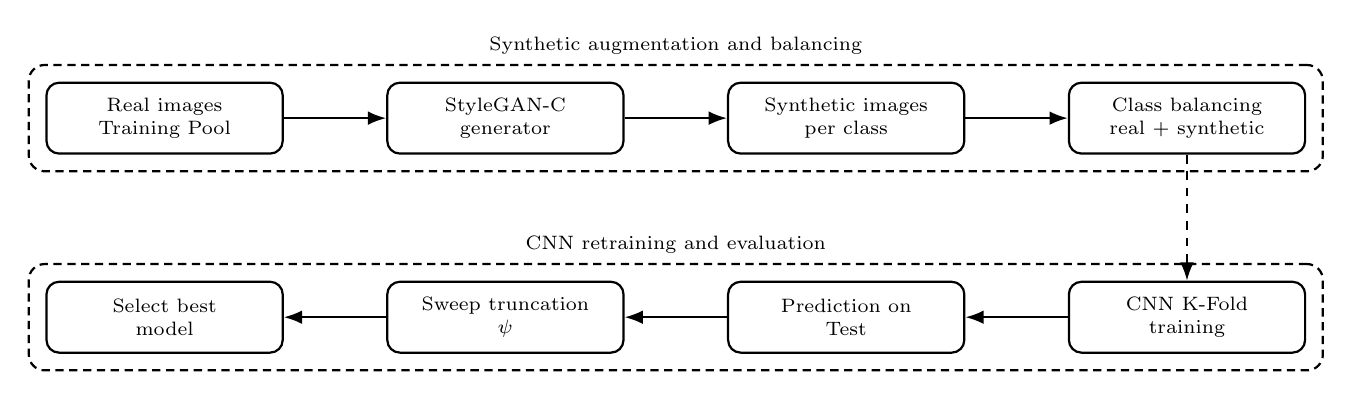
\begin{tikzpicture}[node distance=1.0cm and 1.3cm, >=Latex]

\tikzset{
  block/.style={
    rectangle, rounded corners=1.6mm,
    draw, thick, align=center,
    minimum height=0.9cm, minimum width=3.0cm,
    inner sep=3pt, font=\scriptsize
  },
  arrow/.style={->, thick},
  dashedarrow/.style={->, thick, dashed},
  dframe/.style={draw, thick, densely dashed, rounded corners=2mm, inner sep=6pt}
}

% ==========================
% Top row (left -> right): GAN augmentation
% ==========================
\node[block] (real) {Real images\\Training Pool};
\node[block, right=of real] (gan) {StyleGAN-C\\generator};
\node[block, right=of gan] (synth) {Synthetic images\\per class};
\node[block, right=of synth] (bal) {Class balancing\\real + synthetic};

\draw[arrow] (real) -- (gan);
\draw[arrow] (gan) -- (synth);
\draw[arrow] (synth) -- (bal);

% ==========================
% Bottom row (right -> left): CNN training/evaluation
% (order: training -> sweep -> select -> prediction)
% ==========================
\node[block, below=1.6cm of bal] (train) {CNN K-Fold\\training};
\node[block, left=of train] (psi) {Prediction on\\ Test};
\node[block, left=of psi] (select) {
Sweep truncation\\$\psi$};
\node[block, left=of select] (pred) {Select best\\model};

\draw[arrow] (train) -- (psi);
\draw[arrow] (psi) -- (select);
\draw[arrow] (select) -- (pred);

% Wrap-down arrow
\draw[dashedarrow] (bal.south) to[out=-90, in=90, looseness=0.9] (train.north);

% Frames + labels
\begin{scope}[on background layer]
  \node[dframe, fit=(real)(gan)(synth)(bal)] (frameGen) {};
  \node[dframe, fit=(train)(psi)(select)(pred)] (frameCNN) {};
\end{scope}

\node[font=\scriptsize, anchor=south] at (frameGen.north)
{Synthetic augmentation and balancing};

\node[font=\scriptsize, anchor=south] at (frameCNN.north)
{CNN retraining and evaluation};

\end{tikzpicture}%
}
\caption{Experiment 2C workflow: StyleGAN-C generates class-balanced synthetic images that augment the Training Pool. The CNN is retrained with K-Fold under multiple truncation settings, the best model is selected, and performance is evaluated on the real Test set.}
\label{fig:exp2c_workflow}
\end{figure}



The objective of this experiment \footnote{This experiment is executed twice: once using the complete dataset and once using the reduced. In each case, the conditional StyleGAN-C generator is retrained on the corresponding training split, ensuring that both the classifier and the generative model are matched to the underlying data distribution.} is to determine whether augmenting the training set with class conditional synthetic MRIs generated by StyleGAN-C improves brain tumor classification performance compared to training the classifier on real images alone. To this end, models trained with and without synthetic data are evaluated under strict patient wise data splits and an independent test set, and their macro averaged F1-score are compared.


\subsection{Proposed CNN}

A pre-trained ResNet-50 \cite{he2015deepresiduallearningimage} model is proposed for the classification of brain tumors. The training process involves the following steps:

\begin{enumerate}
    \item \textbf{Initial Training (15 epochs with real and synthetic images)} \\
    The model is first trained for 15 epochs using a combination of real MRI images and synthetic images (if available). During this phase, fine-tuning is applied to all layers of the model, allowing it to learn features from both the pre-trained ImageNet weights and the new MRI images. This helps the model to adapt to the specific characteristics of the brain tumor images, benefiting from the pre-trained knowledge while also learning the domain-specific features.

    \item \textbf{Fine-tuning with Real Images Only (5 epochs)} \\
    After the initial 15 epochs, the model undergoes fine-tuning for an additional 5 epochs, using only real MRI images from the training set. During this phase, all layers of the model are adjusted to better adapt to the real tumor images, ensuring the model’s performance is optimized for classifying brain tumors.

    \item \textbf{Adjustment of the Final Fully Connected (FC) Layer} \\
    Finally, the last fully connected (FC) layer, originally designed to output 1000 classes for ImageNet classification, is modified to output 3 classes. This adjustment allows the model to produce outputs specific to the brain tumor problem, ensuring it can classify MRI images according to the target tumor types (e.g., meningioma, pituitary, glioma).
\end{enumerate}

This approach enables the model to utilize the pre-trained ImageNet features while also fine-tuning the network to specialize in the classification of brain tumors.




\subsection{Baseline: Real images CNN}
Each image is preprocessed as a $256\times256$ single channel slice replicated into three channels to match the ImageNet pretrained backbone. Unless stated otherwise, training uses a single random seed and performance is estimated with $K$-fold cross validation, which reduces sensitivity to random initialization and batching effects.\\

In addition to the cross validated baseline, a single full train model is fitted on the entire training partition (all available training patients) using the same architecture and optimization settings. Its test performance is reported as a point baseline, providing a deterministic reference to compare against the ensemble and augmented configurations considered in Experiment~2C.\\

Furthermore, after the initial training phase, a fine-tuning process is performed on the model using only real images to better adapt the classifier to the specific characteristics of real MRI data. Fine-tuning is conducted for five epochs (\texttt{fine\_tune\_real\_epochs=5}), ensuring that the model continues to leverage the pre-trained weights while refining its performance on real tumor scans. This step enhances the model’s ability to generalize and optimizes its performance specifically for the target classification task.



\subsection{Augmented variant: Real + StyleGAN-C}

The augmented configuration preserves the same network architecture and preprocessing pipeline; the only modification lies in the composition of the training set. In this variant, a StyleGAN-C generator is integrated. First, a fixed pool of synthetic MRIs per class is generated by sampling latent codes $z$ together with class conditioning vectors. Synthetic images are then preprocessed in exactly the same way as real images.\\

For each cross-validation fold, a \emph{balanced} training subset is constructed by mixing real and synthetic images as follows. Let $n_c^{\text{real},(k)}$ denote the number of real training images of class $c$ in fold $k$, and let
\[
n_{\text{target}}^{(k)} = \max_c n_c^{\text{real},(k)}
\]
be the size of the largest real class in that fold. For each class $c$, a deficit is computed as
\[
d_c^{(k)} = n_{\text{target}}^{(k)} - n_c^{\text{real},(k)}.
\]
If $d_c^{(k)} > 0$, then $d_c^{(k)}$ synthetic images of class $c$ are randomly sampled from the pre generated pool and added to the training subset. This procedure yields, for each fold, a training set in which every class has approximately $n_{\text{target}}^{(k)}$ samples when counting real and synthetic images together. Validation and test sets remain strictly real and are never augmented with synthetic images.




\subsection{Evaluation protocol}
For each fold $k$, the model is trained for a fixed number of epochs. At the end of every epoch, validation metrics are computed and the checkpoint with the highest macro-averaged F1-score on the validation set is retained as the ``best'' model for that fold. Using this best checkpoint, the following steps are carried out:
\begin{enumerate}
    \item validation accuracy and macro/weighted Precision, Recall, and F1-score are reported for fold $k$;
    \item predictions are obtained on the test set $\mathcal{D}_{\text{test}}$ (using only real images).
\end{enumerate}

In addition, a \emph{$K$-fold ensemble} is formed on the test set by averaging per-class probabilities across the $K$ best-fold models:
\[
\hat{p}(y \mid x) = \frac{1}{K} \sum_{k=1}^K p^{(k)}(y \mid x),
\]






\subsection{Ablations}

Three complementary ablation studies are conducted, each testing a specific hypothesis:
\begin{itemize}
    \item \textbf{Ablation~1 (CAS):} Tests whether the synthetic images alone contain sufficient class-discriminative information to train a classifier, independently of real data.
    \item \textbf{Ablation~2 (Oversampling):} Tests whether the observed accuracy improvement is due to class balancing alone or to the additional variability introduced by the generator.
    \item \textbf{Ablation~3 (Augmentation strength):} Tests whether the benefit of GAN augmentation persists when compared to strong geometric augmentation on real data.
\end{itemize}

First, \textbf{Ablation~1 (CAS)} evaluates the quality and discriminative utility of StyleGAN-C samples by feeding only generated images to a frozen CNN trained on real data, thus measuring how well synthetic images support classification on their own. Second and third, \textbf{Ablation~2} and \textbf{Ablation~3} compare the effect of class balancing under different image sources and transformation regimes, contrasting real only oversampling and classical augmentation against balanced augmentation with StyleGAN-C. Together, these studies disentangle whether performance gains stem primarily from class rebalancing, from stronger transformations on real data, or from the additional variability introduced by synthetic images.




\subsubsection{Ablation 1: CAS}
The \textit{Classification Accuracy Score} (CAS) quantifies, in isolation, how useful synthetic images are for a fixed discriminative model trained on real data. A frozen CNN is evaluated exclusively on samples generated by StyleGAN-C. CAS thus reflects the discriminative utility of the generated data and enables controlled studies of how truncation \(\psi\) and the number of images per class \(N\) affect downstream classification.\\

For each configuration \((N,\psi)\), the pipeline generates \(N\) images per class, assembles a balanced test with only synthetic images, and computes \(\text{Accuracy (CAS)}\) with the frozen CNN. The process is repeated over a grid of \((N,\psi)\). High CAS indicates that synthetic images preserve clinically relevant patterns consistent with class labels, while systematic CAS trends across \(\psi\) and \(N\) guide the selection of generator settings and help diagnose issues such as mode dropping or artifact-induced biases.

\subsubsection{Ablation 2: Naive Oversampling}

To isolate the effect of class balancing from the specific contribution of synthesized images, this ablation compares a baseline with naive oversampling against a GAN-balanced configuration. In both settings, the same ResNet-50 backbone and K-fold by patient are used, ensuring identical train/validation partitions across conditions. In the \emph{naive oversampling} regime, only real MRI slices are used and minority classes are duplicated with replacement until matching the number of samples of the largest real class within each fold. Any performance difference between these two regimes can therefore be attributed to the additional variability introduced by synthetic augmentation, rather than to class rebalancing itself.


\subsubsection{Ablation 3: Effect of Augmentation Strength}

This ablation complements Ablation~2 by keeping the class balancing strategy fixed to a real images oversampling regime and varying only the strength of classical data augmentation. In this way, it isolates the impact of stronger transformations on the baseline and helps disentangle how much of the performance gain observed in GAN balanced settings could in principle be recovered by applying more aggressive augmentations to real images, without introducing any synthetic data.

Two augmentation regimes are compared:

\begin{itemize}
    \item \textbf{Weak augmentation (baseline).} The weak regime applies only mild geometric transformations, namely a random resized crop with scale in $[0.9, 1.0]$ and aspect ratio in $[0.95, 1.05]$, random horizontal and vertical flips, and small random rotations of up to $\pm 10^\circ$. This setting is intended to introduce limited variability while preserving the anatomical structure of the tumor and surrounding tissue.

    \item \textbf{Strong augmentation.} The strong regime extends the previous transformations with more aggressive perturbations. In addition to flips and rotations of up to $\pm 15^\circ$, it employs a random resized crop with scale in $[0.7, 1.0]$ and aspect ratio in $[0.9, 1.1]$, brightness and contrast jitter, small affine translations and shear, and a mild Gaussian blur. These operations substantially enlarge the space of observed appearances, at the risk of introducing less realistic image configurations.



\end{itemize}

For each regime, a full $K$-fold cross-validation is run on the same patient level splits. By keeping all other factors fixed, this comparison quantifies whether stronger classical augmentation alone can explain the observed improvements, or whether additional gains provided by StyleGAN-C augmentation go beyond what can be achieved with only transformations.


\subsection{Statistical Comparison of Slice-Level Models}
\label{subsec:stat_tests_slice_level}

To assess whether the differences between two competing models were statistically meaningful, a set of paired tests was applied at the MRI slice level. In all cases, the comparison was restricted to the intersection of slices for which both models produced valid outputs. Slices that were present in only one of the models were discarded, ensuring a strict pairing of cases.Two complementary analyses were carried out: (i) a McNemar test on discrete slice level predictions, and (ii) a paired permutation test on slice level negative log-likelihood (NLL) derived from the predicted class probabilities. Both tests were two-sided, and results were interpreted at a significance level of $\alpha = 0.05$.\\


The McNemar test was used to compare the \emph{classification decisions} of two models $A$ and $B$ on the same slices. For each model, a prediction file in \texttt{.csv} format was provided, containing: \texttt{path} (unique slice identifier), \texttt{true} (ground-truth class label) and \texttt{pred} (predicted label). After loading both tables, they were merged by \texttt{path}, and a sanity check ensured that the ground truth labels coincided for every paired slice. From this merged table, each slice was classified into four possible outcomes: both models correct, both models incorrect, only model $A$ correct, or only model $B$ correct. The McNemar test focuses on the \emph{discordant} pairs (slices where exactly one of the two models is correct). Using these counts, a chi-square statistic with continuity correction was computed, together with its associated $p$-value.\\


To exploit the full probabilistic output of the models, a second analysis was performed on slice level negative log-likelihood (NLL). In this case, each prediction file contained, in addition to \texttt{path}, \texttt{patient\_id}, \texttt{true} and \texttt{pred}, one probability column per class. For each slice and each model, the probability assigned to the true class was extracted. The slice level NLL was then computed as the negative logarithm of this probability. The two NLL values (one per model) were merged into a single paired table using \texttt{path}, \texttt{patient\_id} and \texttt{true} as keys. The comparison between models was carried out using a paired permutation test. The null hypothesis assumes that there is no systematic advantage of one model over the other; under this assumption, randomly swapping the NLL values between models within each slice should not change the distribution of average differences.\\

\clearpage
\section{Experiment 3: Classifier Evaluation}

In this experiment, one expert neuroradiologist participated by completing a series of structured surveys designed to evaluate the generated MRI images. The aim is to collect both qualitative feedback and quantitative ratings on diagnostic quality, realism, and clinical utility, in order to assess how well the model is able to produce images that are useful for clinical decision making.



\subsection{Human In the Loop}

To evaluate the quality of the images generated by the StyleGAN-C model, two approaches were used with the expert neuroradiologist: a qualitative assessment, where experts provided feedback on the realism and clinical utility of the images, and a quantitative evaluation, where they judged whether the generated images preserved anatomical structures and tumors realistically, and if they could distinguish real from generated images with a fixed truncation for model retraining.

% Preamble:
% \usetikzlibrary{positioning, arrows.meta, shapes.geometric, fit, backgrounds}

\begin{figure}[H]
\centering
\resizebox{1\textwidth}{!}{%
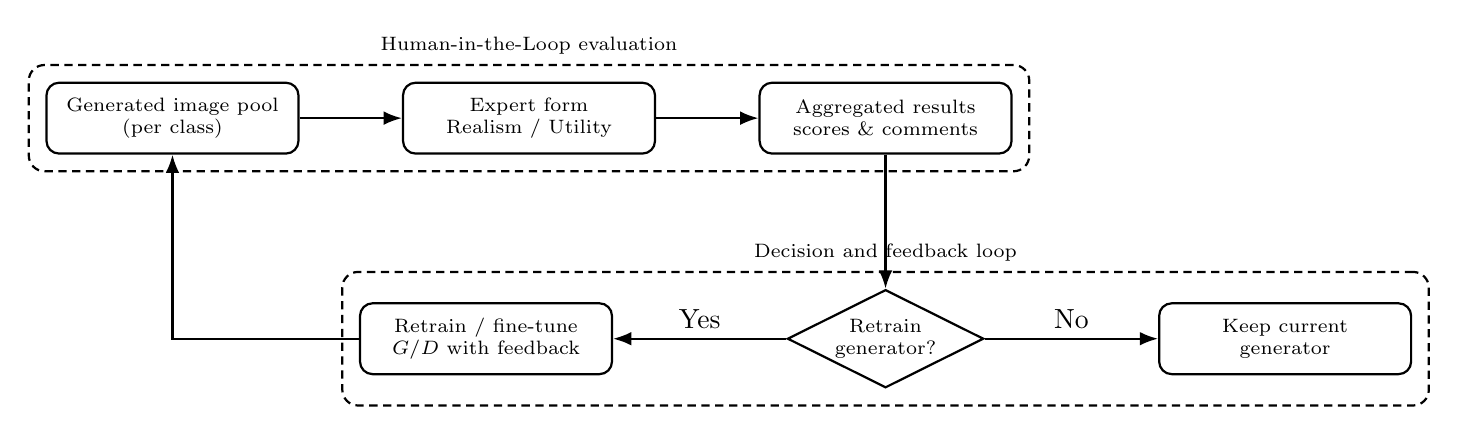
\begin{tikzpicture}[node distance=1.0cm and 1.3cm, >=Latex]

\tikzset{
  block/.style={
    rectangle, rounded corners=1.6mm,
    draw, thick, align=center,
    minimum height=0.9cm, minimum width=3.2cm,
    inner sep=3pt, font=\scriptsize
  },
  decision/.style={
    diamond, draw, thick, aspect=2,
    align=center, inner sep=1pt, font=\scriptsize
  },
  arrow/.style={->, thick},
  dashedarrow/.style={->, thick, dashed},
  dframe/.style={draw, thick, densely dashed, rounded corners=2mm, inner sep=6pt}
}

% ==========================
% Top row (left -> right): Expert evaluation
% ==========================
\node[block] (pool) {Generated image pool\\(per class)};
\node[block, right=of pool] (form) {Expert form\\Realism / Utility};
\node[block, right=of form] (res) {Aggregated results\\scores \& comments};

\draw[arrow] (pool) -- (form);
\draw[arrow] (form) -- (res);

% ==========================
% Bottom row: Decision + loop
%   (SWAPPED: retrain on left, keep on right)
% ==========================
\node[decision, below=1.7cm of res] (dec) {Retrain\\generator?};

\node[block, left=2.2cm of dec] (retrain) {Retrain / fine-tune\\$G/D$ with feedback};
\node[block, right=2.2cm of dec] (keep) {Keep current\\generator};

% Arrows from results to decision (wrap-down)
\draw[arrow] (res.south) to[out=-90, in=90, looseness=0.9] (dec.north);

% Decision branches (labels updated)
\draw[arrow] (dec.west) -- node[above]{Yes} (retrain.east);
\draw[arrow] (dec.east) -- node[above]{No}  (keep.west);

% Loop back to new pool
\draw[arrow] (retrain.west) -| (pool.south);

% ==========================
% Dotted frames + labels
% ==========================
\begin{scope}[on background layer]
  \node[dframe, fit=(pool)(form)(res)] (frameTop) {};
  \node[dframe, fit=(dec)(keep)(retrain)] (frameBot) {};
\end{scope}

\node[font=\scriptsize, anchor=south] at (frameTop.north)
{Human-in-the-Loop evaluation};

\node[font=\scriptsize, anchor=south] at (frameBot.north)
{Decision and feedback loop};

\end{tikzpicture}%
}
\caption{Human-in-the-Loop workflow: experts rate a pool of generated images in terms of realism and clinical utility. Aggregated results determine whether to retrain the generator with feedback or keep the current model.}
\label{fig:hitl_workflow}
\end{figure}



\subsubsection{Quantitative}

The expert neuroradiologists will be asked to provide their opinions on the generated images, specifically regarding their realism and clinical acceptability. This feedback will help guide the retraining of the model by adjusting the preprocessing techniques used to generate the images.

\subsubsection{Qualitative}

To assess the perceptual realism and clinical usefulness of the generated MRIs, a structured survey form is implemented. The first survey is designed to evaluate whether the generated images preserve critical anatomical structures, including tumors, and whether they are perceived as realistic. Additionally, the neuroradiologists are asked whether they can distinguish between real and generated images when the generator is operated at a fixed truncation value. The collected responses serve to determine whether the generated images retain sufficient diagnostic relevance and can be considered suitable for supporting automated classification tasks.


\paragraph{Form~A: Realism \& Diagnostic Utility}
A single sheet instrument presents a randomized grid of images comprising 50\% real test MRIs and 50\% generated StyleGAN-C images, interleaved uniformly and without labels. For each image, specialists record:
\begin{enumerate}[leftmargin=*, itemsep=2pt]
  \item \textbf{Real/Fake judgment}: binary decision (Real or Generated).
  \item \textbf{Confidence (1--5)}: perceived certainty about the judgment (1{=}very low, 5{=}very high).
  \item \textbf{Diagnostic utility (1--5)}: usefulness for clinical interpretation (1{=}not useful, 5{=}highly useful).
\end{enumerate}
This design quantifies the \emph{fooling rate} (fraction of fakes judged real), joint realism/confidence characteristics, and whether generated images preserve salient diagnostic attributes as reflected in utility scores. The sample is stratified so that all three tumor classes are equally represented. 


\subsection{Grad-CAM XAI Evaluation}
Grad-CAM is introduced as a post-hoc explainability tool to help interpret the model’s decision making process. Grad-CAM is applied to the generated MRI images to produce visual heatmaps that highlight the areas the model focuses on when making predictions. The purpose of using Grad-CAM is not to directly improve the classifier’s performance but to enhance the interpretability of the model's behavior. By visualizing which regions of the MRI scans are most important for the model’s classification, Grad-CAM provides insights into whether the model is focusing on relevant anatomical structures or potentially learning spurious correlations.

To complement the quantitative evaluation of the CNN classifier in Experiment~2C, Grad-CAM is employed to obtain visual evidence of how the model arrives at its decisions.

\paragraph{Form B: Evaluation of Grad-CAM’s Utility for Medical Professionals} 
In this final survey, the neuroradiologists are asked to assess whether Grad-CAM helps them interpret and trust the model’s predictions. The survey is same as A and focuses on the following aspects:
\begin{itemize}
    \item Does Grad-CAM help identify the regions of the image that are most important for accurate diagnosis?
    \item Does the visual feedback from Grad-CAM increase the medical professionals' confidence in the model's classifications?
\end{itemize}

A form is generated with pairs of images: one showing the Grad-CAM heatmap and the other showing the same image without the XAI overlay. This allows the experts to compare the visual feedback provided by Grad-CAM with the original images. This evaluation aims to determine if Grad-CAM can serve as an effective tool for improving the explainability and trustworthiness of automated tumor classification systems in a clinical setting.


\chapter{Results}



This chapter presents the results obtained from the experiments conducted with the proposed framework for explainable brain tumor classification. Various configurations and techniques were evaluated, including StyleGAN-C, CNNs and explainable mechanisms. The results are organized by experiment. Additionally, expert evaluation from medical professionals is included to assess the clinical relevance and interpretability of the proposed approach.


\section{Results: Experiment 1}




\subsection{Compute Budget} 

StyleGAN-C was trained separately on the reduced dataset and on the complete dataset, in both cases using an NVIDIA A100 GPU with 80\,GB of VRAM and a runtime environment with 160\,GB of RAM, which corresponds to the most powerful hardware configuration currently available on Google Colab. The training process lasted approximately \textit{8 hours}, reaching \texttt{kimg=600}. This setup enabled efficient processing of high-resolution MRI slices ($256 \times 256$) and ensured stable convergence of the generative model.

\subsection{Generated Images} Figure~\ref{fig:stylegan_conditional_only1} and \ref{fig:stylegan_conditional_only2} show 9 sample images generated by StyleGAN-C, with 3 images per tumor class. Each row corresponds to one of the three tumor types (glioma, meningioma, and pituitary), demonstrating the model's ability to produce class conditional synthetic MRIs that visually resemble real brain tumor images. It is important to note that this version of the generator is conditioned only on tumor class, not on anatomical plane, which may account for certain visual differences in structure and orientation.

\begin{figure}[H]
\centering

\begin{subfigure}[b]{0.48\textwidth}
    \centering
    
\includegraphics[width=\textwidth]{Template-Tesis-dii/img/trunc1complete.png}
    \caption{Complete dataset generator.}
    \label{fig:stylegan_conditional_only1}
\end{subfigure}
\hfill
\begin{subfigure}[b]{0.48\textwidth}
    \centering
    
\includegraphics[width=\textwidth]{Template-Tesis-dii/img/trunc1inge.png}
    \caption{Reduced dataset generator.}
    \label{fig:stylegan_conditional_only2}
\end{subfigure}

\caption{Class-conditional samples generated at truncation $\psi = 1.0$. Rows correspond to tumor classes. The left model was trained on the full dataset, while the right was trained on a reduced subset.}
\label{fig:stylegan_conditional_comparison}
\end{figure}


\subsection{Truncation Effect} 

To analyze the effect of truncation on generation diversity and realism, Figure~\ref{fig:stylegan_class_vs_truncation1} and Figure~\ref{fig:stylegan_class_vs_truncation2} show a grid of synthetic images produced by StyleGAN-C. Each row corresponds to a different tumor class (glioma, meningioma, pituitary), while columns vary the truncation parameter from 0.8 to 1.3. Lower truncation values yield more conservative and realistic outputs, whereas higher values produce more diverse but potentially less plausible samples. 

\begin{figure}[H]
    \centering
    
\includegraphics[width=0.9\textwidth]{Template-Tesis-dii/img/serialinge.png}
    \caption{Grid of images generated by StyleGAN-C across different tumor classes (rows) and truncation values (columns). Reduced Dataset.}
    \label{fig:stylegan_class_vs_truncation1}
\end{figure}

\begin{figure}[H]
    \centering
    
\includegraphics[width=0.9\textwidth]{Template-Tesis-dii/img/serialcomplet.png}
    \caption{Grid of images generated by StyleGAN-C across different tumor classes (rows) and truncation values (columns). Complete Dataset.}
    \label{fig:stylegan_class_vs_truncation2}
\end{figure}


\subsection{Generated Images vs Real Images} Figure~\ref{fig:stylegan_real_vs_fake} compares synthetic and real MR images from the same tumor classes. Each pair of adjacent columns corresponds to a specific class (glioma, meningioma, pituitary), with synthetic samples on the top row and real images on the bottom. 


\begin{figure}[H]
\centering

\includegraphics[width=0.9\textwidth]{Template-Tesis-dii/img/ejemplos/descarga (8).png}
\caption{Comparison between real MR images and synthetic samples. 
The top row shows synthetic images and the bottom row shows real MRIs; pairs of adjacent columns correspond to the three tumor classes.}
\label{fig:stylegan_real_vs_fake}
\end{figure}


\subsection{Latent Inversion} 


Latent inversion was conducted to evaluate the capacity of StyleGAN-C to reconstruct real MR images while enforcing different class embeddings. In Figure~\ref{fig:stylegan_inversion_only}, panel~(a) displays a real pituitary tumor slice from the test set. The following panels~(b)--(d) show reconstructions of the same image using the same optimized latent code but with different class embeddings: glioma, meningioma and pituitary.



\begin{figure}[H]
\centering

\begin{subfigure}[b]{0.33\textwidth}
  \centering
  
\includegraphics[width=\textwidth]{Template-Tesis-dii/img/real_pituitary.png}
  \caption{Real Pituitary.}
  \label{fig:stylegan_inversion_1}
\end{subfigure}
\hfill
\begin{subfigure}[b]{0.33\textwidth}
  \centering
  
\includegraphics[width=\textwidth]{Template-Tesis-dii/img/cf_to_glioma_f02.png}
  \caption{Reconstruction with the class embedding fixed to \emph{glioma}.}
  \label{fig:stylegan_inversion_2}
\end{subfigure}

\vspace{0.5em}

\begin{subfigure}[b]{0.33\textwidth}
  \centering
  
\includegraphics[width=\textwidth]{Template-Tesis-dii/img/cf_to_meningioma_f02.png}
  \caption{Reconstruction with the class embedding fixed to \emph{meningioma}.}
  \label{fig:stylegan_inversion_3}
\end{subfigure}
\hfill
\begin{subfigure}[b]{0.33\textwidth}
  \centering
  
\includegraphics[width=\textwidth]{Template-Tesis-dii/img/cf_to_glioma_f02.png}
  \caption{Reconstruction with the class embedding fixed to \emph{pituitary}.}
  \label{fig:stylegan_inversion_4}
\end{subfigure}

\caption{Example of StyleGAN-C inversion on a held-out test MRI. 
Panel~(a) shows the real target image. Panels~(b)--(d) show reconstructions obtained 
by optimizing the latent code while constraining the generator to each tumor class 
(glioma, meningioma, and pituitary, respectively).}
\label{fig:stylegan_inversion_only}
\end{figure}



\subsection{Quantitative Metrics}

Image quality metrics are computed using the conditional generator trained exclusively on the reduced training set, with all generator weights kept fixed during evaluation. At test time, real MRI slices from the held-out testing set are provided as inputs, projected/inverted into the generator's latent space through the inversion module, and re synthesized as class conditioned reconstructions for each target class. Consequently, all evaluated generations correspond to unseen test examples, enabling an unbiased assessment of generalization. Pairwise metrics (PSNR, SSIM, LPIPS) compare each class conditioned reconstruction to its original test image, whereas the set-level metric (FID) measures distributional similarity between real test images and generated images within each class.

\subsubsection{Inversion Images}

\begin{table}[H]
\centering
\caption{Diagonal reconstruction metrics (real class = generated class). PSNR and SSIM are higher-is-better, LPIPS and FID are lower-is-better. PSNR/SSIM/LPIPS are reported as mean $\pm$ std over paired samples, while FID is computed at the set level per class.}
\label{tab:diag_metrics_with_fid}
\begin{tabular}{lcccc}
\toprule
\textbf{Real class} & \textbf{PSNR (dB)} & \textbf{SSIM} & \textbf{LPIPS} & \textbf{FID} \\
\midrule
glioma      & $15.461 \pm 1.856$ & $0.543 \pm 0.093$ & $0.211 \pm 0.071$ & 123.909 \\
meningioma  & $13.908 \pm 1.641$ & $0.474 \pm 0.096$ & $0.280 \pm 0.083$ & 142.130 \\
pituitary   & $13.300 \pm 1.633$ & $0.377 \pm 0.091$ & $0.264 \pm 0.081$ & 168.521 \\
\midrule
total       & $14.427 \pm 1.976$ & $0.478 \pm 0.116$ & $0.245 \pm 0.083$ & 103.958 \\
\bottomrule
\end{tabular}
\end{table}


\begin{table}[ht]
\centering
\caption{Pairwise metrics for all real-to-generated class combinations.}
\label{tab:all_combos_psnr_ssim_lpips}
\begin{tabular}{llccc}
\toprule
\textbf{Real class} & \textbf{Gen class} & \textbf{PSNR (dB)} & \textbf{SSIM} & \textbf{LPIPS} \\
\midrule
glioma     & glioma     & 15.461 & 0.543 & 0.211 \\
glioma     & meningioma & 14.416 & 0.495 & 0.257 \\
glioma     & pituitary  & 13.887 & 0.439 & 0.238 \\
meningioma & glioma     & 14.041 & 0.484 & 0.271 \\
meningioma & meningioma & 13.908 & 0.474 & 0.280 \\
meningioma & pituitary  & 13.204 & 0.429 & 0.306 \\
pituitary  & glioma     & 12.826 & 0.369 & 0.294 \\
pituitary  & meningioma & 12.533 & 0.360 & 0.314 \\
pituitary  & pituitary  & 13.300 & 0.377 & 0.264 \\
\bottomrule
\end{tabular}
\end{table}

\subsubsection{Images reduced data set generator images}

As a result, when comparing the distribution of real training images and the synthetic images generated by StyleGAN-C on the reduced dataset, the best global FID was obtained for truncation $\psi = 1.0$ with a score of 46.08 (Table~\ref{tab:fid_global_truncation}).


\begin{table}[H]
\centering
\caption{Global FID as a function of the truncation parameter $\psi$ and 600 samples per class.}
\label{tab:fid_global_truncation}
\begin{tabular}{lc}
\toprule
\textbf{Truncation $\psi$} & \textbf{FID (global)} \\
\midrule
0.9 & 46.239 \\
1.0 & 46.08 \\
1.1 & 49.192 \\
1.2 & 54.024 \\
1.3 & 58.296 \\
1.4 & 67.509 \\
\bottomrule
\end{tabular}
\end{table}

\clearpage
\section{Results: Experiment 2A}

This experiment presents the performance metrics of the classification model by inference (LPIPS based), in comparison with a CNN baseline. Unlike the other experiments, this setup performs classification at the patient level rather than at the slice level and uses only one slice per patient. This decision was taken due to the high computational cost associated with applying generative inversion and LPIPS  inference to every individual slice. Table~\ref{tab:ensemble_overall} reports the global performance metrics for all three methods, while Table~\ref{tab:ensemble_confusion} shows the corresponding patient-level confusion matrices.

\begin{table}[H]
\centering
\caption{Patient-level performance of the CNN and LPIPS-based inference by generation (68 patients).}
\label{tab:ensemble_overall}
\begin{tabular}{lcccc}
\toprule
Method & Accuracy & Precision (macro) & Recall (macro) & F1-score (macro) \\
\midrule
CNN           & 0.838 & 0.864 & 0.858 & 0.852 \\
LPIPS        & 0.765 & 0.757 & 0.760 & 0.757 \\
\bottomrule
\end{tabular}
\end{table}


\begin{table}[H]
\centering
\caption{Confusion matrices at patient level for the CNN baseline and LPIPS-based inference by generation (rows = true class, columns = predicted class).}
\label{tab:ensemble_confusion}
\begin{tabular}{lccc}
\toprule
 & \multicolumn{3}{c}{Predicted class} \\
\cmidrule(lr){2-4}
True class / Method & glioma & meningioma & pituitary \\
\midrule
\multicolumn{4}{l}{\textbf{CNN (prob-based aggregation)}} \\
glioma     & 21 & 8 & 0 \\
meningioma & 2  & 19 & 0 \\
pituitary  & 0  & 1  & 17 \\
\midrule
\multicolumn{4}{l}{\textbf{LPIPS (normalized inference by generation)}} \\
glioma     & 24 & 2 & 3 \\
meningioma & 6  & 13 & 2 \\
pituitary  & 0  & 3  & 15 \\
\bottomrule
\end{tabular}
\end{table}


\subsection{Counterfactual Videos}

To support visual explainability and clinical interpretability, counterfactual videos were generated for each test patient. These videos show how a real MRI slice would appear if it belonged to a different tumor class, by interpolating the latent space and conditioning the generator on alternative class embeddings. For each patient, the first available slice is selected as input, and a total of 120 frames are generated by linearly interpolating from the original latent code to the class-conditional projection. Each patient is associated with three class conditional videos (one per tumor type) revealing fine or pronounced changes in tumor structure and surrounding tissue throughout the transformation.


\begin{figure}[H]
    \centering
    \includegraphics[width=\textwidth]{Template-Tesis-dii/img/videoexample.png}
    \caption{Counterfactual trajectory for a glioma case (glioma$\rightarrow$glioma). The 120 frames show a latent interpolation that preserves the glioma class while progressively moving towards the corresponding class prototype.}
    \label{fig:counterfactual_120frames}
\end{figure}


\begin{figure}[ht]
    \centering
    \includegraphics[width=\textwidth]{Template-Tesis-dii/img/videoexamplepituitary.png}
    \caption{Counterfactual trajectory for a glioma case (glioma$\rightarrow$pituitary). The 120 frames show a latent interpolation that preserves the glioma class while progressively moving towards the corresponding class prototype.}
    \label{fig:counterfactual_120frames1}
\end{figure}


\clearpage

\section{Results: Experiment 2B}



\begin{enumerate}
    \item \textbf{CNN}: SVM trained on penultimate-layer features from the fine tuned tumor ResNet-50.
    \item \textbf{Encoder}: SVM trained on embeddings produced by the supervised encoder.
    \item \textbf{e4e}: SVM trained on W\textsuperscript{+} latent codes extracted by the e4e encoder pre-trained on StyleGAN2-FFHQ and fine tuned on the tumor dataset.
\end{enumerate}


\subsection{SVM Metrics}

Table~\ref{tab:exp2b_all_metrics} summarizes the global performance on the test set in terms of accuracy and macro-averaged precision, recall and F1-score.

\begin{table}[ht]
    \centering
    \caption{Per-class and global metrics on the test set for the three feature configurations. 
    For class rows, precision/recall/F1-score are per-class; for the total row, they correspond to macro-averaged precision, recall and F1-score.}
    \label{tab:exp2b_all_metrics}
    \begin{tabular}{llcccc}
        \toprule
        Setting        & Class       & Precision & Recall  & F1-score & Accuracy \\
        \midrule
        % ============== CNN-only ==============
        \multirow{4}{*}{CNN}
                       & glioma      & 0.961     & 0.939   & 0.950    & --       \\
                       & meningioma  & 0.847     & 0.887   & 0.866    & --       \\
                       & pituitary   & 0.967     & 0.970   & 0.969    & --       \\
        \cmidrule(lr){2-6}
                       & \textbf{total}     
                                    & \textbf{0.925} 
                                              & \textbf{0.932} 
                                                      & \textbf{0.928} 
                                                              & \textbf{0.9374}   \\
        \midrule
        % ============== Encoder-only ==========
        \multirow{4}{*}{Encoder}
                       & glioma      & 0.970     & 0.948   & 0.959    & --       \\
                       & meningioma  & 0.851     & 0.912   & 0.881    & --       \\
                       & pituitary   & 0.985     & 0.970   & 0.978    & --       \\
        \cmidrule(lr){2-6}
                       & \textbf{total}     
                                    & \textbf{0.935} 
                                              & \textbf{0.944} 
                                                      & \textbf{0.939} 
                                                              & \textbf{0.9473}   \\ 
        \midrule
        % ============== E4E-only ==============
        \multirow{4}{*}{e4e}
                       & glioma      & 0.864     & 0.852   & 0.858    & --       \\
                       & meningioma  & 0.643     & 0.696   & 0.668    & --       \\
                       & pituitary   & 0.931     & 0.897   & 0.914    & --       \\
        \cmidrule(lr){2-6}
                       & \textbf{total}     
                                    & \textbf{0.813} 
                                              & \textbf{0.815} 
                                                      & \textbf{0.813} 
                                                              & \textbf{0.8321}   \\
        \bottomrule
    \end{tabular}
\end{table}


The supervised encoder achieves the best overall performance, with an accuracy of 0.9473 and a macro F1-score of 0.9390, slightly outperforming the CNN features (accuracy = 0.9374, macro F1 = 0.9280). In contrast, the e4e configuration yields substantially lower performance (accuracy = 0.8321, macro F1 = 0.8130).


\subsection{Confusion matrices}

Table~\ref{tab:cm_all_models} reports the confusion matrices for the three feature configurations, with rows corresponding to the true class and columns to the predicted class.

\begin{table}[ht]
    \centering
    \caption{Confusion matrices for the three feature configurations on the test set (rows = true class, columns = predicted class).}
    \label{tab:cm_all_models}
    \begin{tabular}{llccc}
        \toprule
        Setting        & True class & glioma & meningioma & pituitary \\
        \midrule
        % ============== CNN-only ==============
        \multirow{3}{*}{CNN}
                       & glioma      & 419   & 24        & 3         \\
                       & meningioma  & 16    & 172       & 6         \\
                       & pituitary   & 1     & 7         & 263       \\
        \midrule
        % ============== Encoder-only ==========
        \multirow{3}{*}{Encoder}
                       & glioma      & 423   & 23        & 0         \\
                       & meningioma  & 13    & 177       & 4         \\
                       & pituitary   & 0     & 8         & 263       \\
        \midrule
        % ============== E4E-only ==============
        \multirow{3}{*}{e4e}
                       & glioma      & 380   & 58        & 8         \\
                       & meningioma  & 49    & 135       & 10        \\
                       & pituitary   & 11    & 17        & 243       \\
        \bottomrule
    \end{tabular}
\end{table}

Overall, the CNN and encoder configurations exhibit similar error patterns, with most mistakes occurring between glioma and meningioma and very few pituitary tumors being confused with the other classes. The encoder model slightly reduces the number of misclassifications for glioma and meningioma compared with the CNN baseline, in line with its higher macro F1-score. In contrast, the e4e configuration produces substantially more errors for all three classes, particularly an increased confusion of meningioma and pituitary with glioma, which is consistent with its lower overall accuracy and macro F1-score.
\subsection{PCA Analysis}

Figure~\ref{fig:pca_exp2b} presents the three-dimensional PCA projections of the feature spaces obtained from the three configurations, separately for the training and test splits. Each point corresponds to an MRI slice and is color coded according to the tumor class, allowing visual inspection of how the different representations distribute the classes in a low dimensional space. Table~\ref{tab:pca_variance} reports the proportion of variance explained by the first three principal components for each feature space and split. Together, the figure and the table summarize the global geometric structure of the learned embeddings and how much of their variability is captured by the leading PCA directions.


\begin{table}[H]
    \centering
    \caption{Explained variance ratio of the first three principal components
             for each feature configuration. The \emph{Shape} column indicates
             the number of samples and feature dimensionality used to fit PCA.}
    \label{tab:pca_variance}
    \begin{tabular}{llccccc}
        \toprule
        Features      & Split & Shape              & PC1    & PC2    & PC3    & SUM(PC1--3) \\
        \midrule
        \multirow{2}{*}{Encoder} 
                      & train & \(2153 \times 512\)  & 0.5893 & 0.4074 & 0.0007 & 0.9974 \\
                      & test  & \(911 \times 512\)   & 0.5809 & 0.4128 & 0.0016 & 0.9952 \\
        \midrule
        \multirow{2}{*}{CNN} 
                      & train & \(2153 \times 2048\) & 0.3698 & 0.3018 & 0.0501 & 0.7216 \\
                      & test  & \(911 \times 2048\)  & 0.3788 & 0.2677 & 0.0454 & 0.6918 \\
        \midrule
        \multirow{2}{*}{e4e} 
                      & train & \(2153 \times 7168\) & 0.3347 & 0.1946 & 0.1337 & 0.6630 \\
                      & test  & \(911 \times 7168\)  & 0.3598 & 0.1780 & 0.1479 & 0.6857 \\
        \bottomrule
    \end{tabular}
\end{table}



\begin{figure}[h]
    \centering

    % ===== Row 1 =====
    \begin{subfigure}[b]{0.4\textwidth}
        \centering
        
\includegraphics[width=\textwidth]{Template-Tesis-dii/img/ejemplos/pca/pcwtrain.png}
        \caption{Encoder (train)}
        \label{fig:pca_w_train}
    \end{subfigure}
    \hfill
    \begin{subfigure}[b]{0.4\textwidth}
        \centering
        
\includegraphics[width=\textwidth]{Template-Tesis-dii/img/ejemplos/pca/pcawtest.png}
        \caption{Encoder (test)}
        \label{fig:pca_w_test}
    \end{subfigure}

    \vspace{0.5em}

    % ===== Row 2 =====
    \begin{subfigure}[b]{0.4\textwidth}
        \centering
        
\includegraphics[width=\textwidth]{Template-Tesis-dii/img/ejemplos/pca/pcacnntrain.png}
        \caption{CNN (train)}
        \label{fig:pca_cnn_train}
    \end{subfigure}
    \hfill
    \begin{subfigure}[b]{0.4\textwidth}
        \centering
        
\includegraphics[width=\textwidth]{Template-Tesis-dii/img/ejemplos/pca/pcacnntest.png}
        \caption{CNN (test)}
        \label{fig:pca_cnn_test}
    \end{subfigure}

    \vspace{0.5em}

    % ===== Row 3 =====
    \begin{subfigure}[b]{0.4\textwidth}
        \centering
        
\includegraphics[width=\textwidth]{Template-Tesis-dii/img/e4epcatrain.png}
        \caption{e4e (train)}
        \label{fig:pca_fusion_train}
    \end{subfigure}
    \hfill
    \begin{subfigure}[b]{0.4\textwidth}
        \centering
        
\includegraphics[width=\textwidth]{Template-Tesis-dii/img/e4epcatest.png}
        \caption{e4e (test)}
        \label{fig:pca_fusion_test}
    \end{subfigure}

    \caption{PCA projections of the encoder, CNN and e4e feature spaces on the training (left column) and test (right column) splits. Each point corresponds to an MRI slice, color coded by tumor class.}
    \label{fig:pca_exp2b}
\end{figure}

\clearpage


\section{Results: Experiment 2C}
\label{sec:results-augmentation}



Experiment 2C evaluates whether class conditional synthetic augmentation with StyleGAN-C improves tumor classification performance under patient level data splits. The study compares real only training against augmented synthetic training across multiple folds, using both the complete and reduced datasets. Additionally, ablation studies explore the influence of truncation levels (\(\psi\)), augmentation strength, CAS, and oversampling baselines.


\begin{table}[ht]
\centering
\caption{CNN Training and augmentation hyperparameters used in all experiments.}
\label{tab:hyperparams}
\begin{tabular}{ll}
\toprule
Hyperparameter                    & Value \\
\midrule
Backbone architecture            & ResNet-50 (ImageNet-pretrained) \\
Input resolution                 & $256\times256$\\
Learning rate                    & $1\times10^{-4}$ \\
Weight decay                     & $1\times10^{-4}$ \\
Batch size                       & 32 \\
Training epochs per fold         & 20 \\
Cross-validation folds $K$       & $K=3$ and $K=5$  \\
Split strategy                   & StratifiedGroupKFold by patient ID \\
GAN backbone                     & Class-conditional StyleGAN2-ADA \\
GAN truncation $\psi$           & $\psi \in \{0.8,0.9,1.0,1.1,1.2,1.3, 1.4, 1.5\}$  \\
Random seed                      & $122$ \\
\bottomrule
\end{tabular}
\end{table}

\paragraph{Dataset comparison}
Parallel experiments were conducted using both the complete and reduced datasets to evaluate the robustness and generalization capabilities of the classification model under varying levels of data availability. Both configurations followed the same experimental protocol, including training with real samples and synthetic augmentation. This setup enables a direct comparison of model performance depending on the amount of real data available and highlights the relative benefits of incorporating generated samples.

\subsection{Complete Dataset}
\label{subsec:aug-primary}

The complete dataset setting uses all available MRI slices from the dataset, providing the classifier with the maximum amount of real data.




\subsubsection{Cross Validation Summary}

The tables present the performance metrics of the model across different cross-validation folds. They compare the results for real images training and GAN augmented training with various truncation values, showing the mean and standard deviation for each metric.

\begin{table}[H]
\centering
\small
\caption{TEST macro metrics for 3-fold experiments: real-only vs.\ GAN-balanced ($\psi=1.4$). Values are mean $\pm$ std across folds.}
\label{tab:3k_test_macro}
\begin{tabular}{lcccc}
\toprule
Setting & Accuracy & Precision (macro) & Recall (macro) & F1 (macro) \\
\midrule
Real-only        & $0.930 \pm 0.014$ & $0.920 \pm 0.016$ & $0.927 \pm 0.006$ & $0.922 \pm 0.013$ \\
GAN ($\psi=1.4$) & $0.945 \pm 0.003$ & $0.940 \pm 0.002$ & $0.938 \pm 0.003$ & $0.939 \pm 0.002$ \\
\bottomrule
\end{tabular}
\end{table}
\begin{table}[H]
\centering
\caption{TEST performance for 5-fold runs using macro metrics (mean $\pm$ standard deviation across folds).}
\label{tab:test_5fold_macro_real_vs_gan}
\begin{tabular}{lcccc}
\toprule
Setting & Accuracy & Precision (macro) & Recall (macro) & F1 (macro) \\
\midrule
Real-only         & $0.941 \pm 0.011$ & $0.934 \pm 0.014$ & $0.935 \pm 0.013$ & $0.934 \pm 0.013$ \\
GAN ($\psi=1.3$)  & $0.941 \pm 0.010$ & $0.932 \pm 0.014$ & $0.937 \pm 0.009$  & $0.934 \pm 0.011$ \\
GAN ($\psi=1.4$)  & $0.948 \pm 0.002$ & $0.941 \pm 0.004$ & $0.942 \pm 0.006$ & $0.941 \pm 0.003$ \\
GAN ($\psi=1.5$)  & $0.937 \pm 0.003$ & $0.926 \pm 0.005$ & $0.933 \pm 0.005$ & $0.929 \pm 0.004$ \\
\bottomrule
\end{tabular}
\end{table}



\subsubsection{Ensemble Evaluation}

The tables present the performance metrics of the ensemble model, which aggregates predictions across multiple cross-validation folds to improve performance and robustness.


\begin{table}[H]
    \centering
    \caption{5 fold Overall macro-averaged performance for the CNN ensemble with different truncation values $\psi$.}
    \label{tab:macro_overall_truncation}
    \begin{tabular}{lcccc}
        \toprule
        Setting        & Accuracy & Precision (macro) & Recall (macro) & F1 (macro) \\
        \midrule
        Real ensemble  & 0.947 & 0.940 & 0.943 & 0.941 \\
        $\psi = 1.3$   & 0.957 & 0.952 & 0.954 & 0.953 \\
        $\psi = 1.4$   & 0.956 & 0.953 & 0.950 & 0.951 \\
        $\psi = 1.5$   & 0.952 & 0.943 & 0.949 & 0.946 \\
        \bottomrule
    \end{tabular}
\end{table}

\begin{table}[H]
\centering
\caption{Per-class test performance of the 3-fold ensemble for real-only vs.\ GAN-augmented training.}
\label{tab:test_ensemble_per_class_3fold_real_vs_gan}
\begin{tabular}{lcccccc}
\toprule
Setting      & Class       & Precision & Recall & F1-score & Accuracy & Test samples \\
\midrule
Real-only    & Glioma      & $0.965$ & $0.930$ & $0.947$ & --      & $446$ \\
Real-only    & Meningioma  & $0.850$ & $0.907$ & $0.878$ & --      & $194$ \\
Real-only    & Pituitary   & $0.974$ & $0.985$ & $0.980$ & --      & $271$ \\
Real-only    & \textbf{Total}
             & $\mathbf{0.930}$ & $\mathbf{0.941}$ & $\mathbf{0.935}$ & $\mathbf{0.942}$ & $\mathbf{911}$ \\
\midrule
GAN ($\psi=1.4$) & Glioma     & $0.953$ & $0.962$ & $0.958$ & --      & $446$ \\
GAN ($\psi=1.4$) & Meningioma & $0.906$ & $0.897$ & $0.902$ & --      & $194$ \\
GAN ($\psi=1.4$) & Pituitary  & $0.970$ & $0.963$ & $0.967$ & --      & $271$ \\
GAN ($\psi=1.4$) & \textbf{Total}
             & $\mathbf{0.943}$ & $\mathbf{0.941}$ & $\mathbf{0.942}$ & $\mathbf{0.948}$ & $\mathbf{911}$ \\
\bottomrule
\end{tabular}
\end{table}

\begin{table}[H]
\centering
\small
\caption{Per-class test performance of the 5-fold ensemble for real-only vs.\ GAN-balanced ($\psi=1.4$).}
\label{tab:ensemble5k_perclass_real_vs_gan14}
\begin{tabular}{lcccccc}
\toprule
Setting & Class & Precision & Recall & F1-score & Accuracy & Test samples \\
\midrule
Real-only        & Glioma     & 0.955 & 0.953 & 0.954 & --     & 446 \\
Real-only        & Meningioma & 0.881 & 0.912 & 0.896 & --     & 194 \\
Real-only        & Pituitary  & 0.985 & 0.963 & 0.974 & --     & 271 \\
Real-only        & \textbf{Total} 
                 & \textbf{0.940} & \textbf{0.943} & \textbf{0.941} & \textbf{0.947} & \textbf{911} \\
\midrule
GAN ($\psi=1.4$) & Glioma     & 0.953 & 0.964 & 0.959 & --     & 446 \\
GAN ($\psi=1.4$) & Meningioma & 0.912 & 0.907 & 0.910 & --     & 194 \\
GAN ($\psi=1.4$) & Pituitary  & 0.993 & 0.978 & 0.985 & --     & 271 \\
GAN ($\psi=1.4$) & \textbf{Total} 
                 & \textbf{0.953} & \textbf{0.950} & \textbf{0.951} & \textbf{0.956} & \textbf{911} \\
\bottomrule
\end{tabular}
\end{table}

\subsection{Reduced Dataset}

The reduced dataset is filtered to exclude MRI slices with poor quality or images where the tumor is not clearly visible, ensuring that only relevant and high-quality data is used for training.

\subsubsection{Baseline}

As a reference configuration, the classifier was trained on all available internal slices and evaluated once on the test set, yielding a single baseline operating point.





\begin{table}[ht]
\centering
\caption{Full-train test performance (macro metrics).}
\begin{tabular}{lccccc}
\toprule
\textbf{Setting} & \textbf{N} & \textbf{Accuracy} & \textbf{Precision (macro)} & \textbf{Recall (macro)} & \textbf{F1 (macro)} \\
\midrule
Full train 
& 702 
& 0.934 
& 0.922 
& 0.933 
& 0.927 \\
\bottomrule
\end{tabular}
\label{tab:full_train_macro}
\end{table}


\subsubsection{Cross Validation Summary}

\begin{table}[H]
\centering
\caption{Test performance for 5-fold experiments with real-only training and synthetic augmentation using different truncation $\psi$.}
\label{tab:test_truncation}
\begin{tabular}{lcccc}
\toprule
Setting        & Accuracy           & Precision (macro)    & Recall (macro)       & F1 (macro)          \\
\midrule
Real only      & $0.948 \pm 0.009$  & $0.934 \pm 0.010$    & $0.945 \pm 0.012$    & $0.939 \pm 0.011$   \\
$\psi = 0.8$   & $0.950 \pm 0.006$  & $0.938 \pm 0.007$    & $0.946 \pm 0.006$    & $0.942 \pm 0.007$   \\
$\psi = 1.1$   & $0.953 \pm 0.009$  & $0.941 \pm 0.011$    & $0.950 \pm 0.011$    & $0.945 \pm 0.011$   \\
$\psi = 1.2$   & $0.952 \pm 0.008$  & $0.940 \pm 0.012$    & $0.948 \pm 0.006$    & $0.944 \pm 0.009$   \\
$\psi = 1.3$   & $0.954 \pm 0.007$  & $0.944 \pm 0.007$    & $0.949 \pm 0.011$    & $0.946 \pm 0.009$   \\
$\psi = 1.4$   & $0.950 \pm 0.005$  & $0.940 \pm 0.006$    & $0.944 \pm 0.006$    & $0.942 \pm 0.006$   \\
\bottomrule
\end{tabular}
\end{table}

\subsubsection{Ensemble Evaluation}

\begin{table}[H]
\centering
\caption{Test performance of the 5-fold ensemble for real-only vs.\ GAN training with truncation $\psi = 1.3$.}
\label{tab:test_ensemble_per_class_5fold}
\begin{tabular}{ccccccc}
\toprule
Setting      & Class      & Precision & Recall & F1-score & Accuracy & Test samples \\
\midrule
Real-only    & Glioma     & $0.964$ & $0.952$ & $0.958$ & --      & $312$ \\
Real-only    & Meningioma & $0.884$ & $0.915$ & $0.899$ & --      & $141$ \\
Real-only    & Pituitary  & $0.980$ & $0.976$ & $0.978$ & --      & $249$ \\
Real-only    & \textbf{Total} 
             & $\mathbf{0.943}$ & $\mathbf{0.948}$ & $\mathbf{0.945}$ & $\mathbf{0.953}$ & $\mathbf{702}$ \\
\midrule
$\psi = 1.3$ & Glioma     & $0.958$ & $0.962$ & $0.960$ & --      & $312$ \\
$\psi = 1.3$ & Meningioma & $0.909$ & $0.922$ & $0.915$ & --      & $141$ \\
$\psi = 1.3$ & Pituitary  & $0.992$ & $0.980$ & $0.986$ & --      & $249$ \\
$\psi = 1.3$ & \textbf{Total} 
             & $\mathbf{0.953}$ & $\mathbf{0.954}$ & $\mathbf{0.954}$ & $\mathbf{0.960}$ & $\mathbf{702}$ \\
\bottomrule
\end{tabular}
\end{table}

\begin{table}[ht]
    \centering
    \caption{Overall macro-averaged performance for the CNN ensemble with different truncation values $\psi$.}
    \label{tab:macro_overall_truncation_inttest}
    \begin{tabular}{lcccc}
        \toprule
        Setting        & Accuracy & Precision (macro) & Recall (macro) & F1 (macro) \\
        \midrule
        Real ensemble  & 0.953 & 0.939 & 0.952 & 0.945 \\
        $\psi = 0.8$   & 0.954 & 0.942 & 0.950 & 0.946 \\
        $\psi = 1.1$   & 0.956 & 0.943 & 0.954 & 0.948 \\
        $\psi = 1.2$   & 0.960 & 0.949 & 0.957 & 0.953 \\
        $\psi = 1.3$   & 0.960 & 0.953 & 0.954 & 0.954 \\
        $\psi = 1.4$   & 0.953 & 0.943 & 0.948 & 0.945 \\
        \bottomrule
    \end{tabular}
\end{table}

\subsection{Ablation}

Different ablations of data augmentation were performed to determine whether the improvements in metrics were due to class balancing or the quality of the synthetic images. To investigate this, ablation studies were conducted with class balancing using duplicated images, as well as weak and strong geometric variations. Additionally, the CAS metric was included to quantify the quality of the generated images and assess how useful these images are for training the model.

\subsubsection{Ablation 1: CAS}


\begin{table}[H]
\centering
\caption{CAS macro metrics on synthetic-only test for different $N$ and truncation $\psi$ (rounded to three decimals).}
\label{tab:cas_synth_metrics_boxed}
\begin{tabular}{cccccc}
\toprule

$N$ & $\psi$ & Accuracy & Precision (macro) & Recall (macro) & F1 (macro) \\
\midrule
400 & 0.8 & 0.905 & 0.887 & 0.908 & 0.894 \\
400 & 1.0 & 0.923 & 0.906 & 0.923 & 0.912 \\
400 & 1.2 & 0.913 & 0.897 & 0.911 & 0.902 \\
400 & 1.4 & 0.909 & 0.892 & 0.889 & 0.890 \\
\midrule
600 & 0.8 & 0.895 & 0.875 & 0.892 & 0.880 \\
600 & 1.0 & 0.899 & 0.878 & 0.889 & 0.883 \\
600 & 1.2 & 0.906 & 0.886 & 0.891 & 0.888 \\
600 & 1.4 & 0.906 & 0.888 & 0.886 & 0.887 \\
\bottomrule
\end{tabular}
\end{table}


\begin{figure}[H]
  \centering
  
\includegraphics[width=0.75\textwidth]{Template-Tesis-dii/img/cas.png}
  \caption{Macro F1 on synthetic-only CAS vs.\ truncation $\psi$  (higher is better).}
  \label{fig:cas_macro_f1_truncation}
\end{figure}





\subsubsection{Ablation 2: Oversample Augmentation}

\begin{table}[H]
\centering
\caption{Slice-level performance of the real-only oversampling ensemble baseline on the 5k test set ($n = 702$).}
\begin{tabular}{lc}
\toprule
Metric & Value \\
\midrule
Accuracy             & 0.934 \\
Precision (macro)    & 0.918 \\
Recall (macro)       & 0.925 \\
F1-score (macro)     & 0.921 \\
Precision (weighted) & 0.937 \\
Recall (weighted)    & 0.934 \\
F1-score (weighted)  & 0.935 \\
\bottomrule
\end{tabular}
\label{tab:exp2c_b1_oversample}
\end{table}



\subsubsection{Ablation 3: Weak vs Strong Augmentation}


\begin{table}[H]
\centering
\caption{Comparison between weak and strong augmentation regimes (Test, $n = 702$ slices). Strong augmentation consistently outperforms the weak baseline.}
\begin{tabular}{lccc}
\toprule
Metric & Weak aug & Strong aug & $\Delta$ (Strong -- Weak) \\
\midrule
Accuracy             & 0.932 & 0.959 & +0.027 \\
Precision (macro)    & 0.915 & 0.951 & +0.037 \\
Recall (macro)       & 0.921 & 0.953 & +0.031 \\
F1-score (macro)     & 0.918 & 0.952 & +0.034 \\
Precision (weighted) & 0.934 & 0.959 & +0.026 \\
Recall (weighted)    & 0.932 & 0.959 & +0.027 \\
F1-score (weighted)  & 0.932 & 0.959 & +0.026 \\
\bottomrule
\end{tabular}
\label{tab:exp2c_b2_weak_vs_strong}
\end{table}










\subsection{Statistical Tests}

Statistical tests were performed to assess the significance of model performance across different datasets. The McNemar test compares slice level performance between single run and ensemble models, as well as real only vs. GAN-augmented ensembles. The NLL comparison between the reduced and complete datasets reveals the effect of dataset quality and size on the model's confidence and generalization, with significant differences observed for certain tumor classes.

\begin{table}[ht]
\centering
\caption{Slice-level performance for McNemar test P-value}
\begin{tabular}{lcc}
\toprule
\textbf{Comparison} & \textbf{Complete Dataset} & \textbf{Reduced Dataset} \\
\midrule
Single Run GAN vs Ensemble GAN & 0.000308 & 0.002967 \\
Ensemble Real vs Ensemble GAN & 0.080 & 0.332 \\
\bottomrule
\end{tabular}
\label{tab:mcnemar_comparison_side_by_side}
\end{table}


\begin{table}[ht]
\centering
\caption{Global and per-class slice-level NLL comparison for the reduced and complete datasets (A: real-only, B: synthetic) N(=\#Reducedimages/\#Completeimages).}
\begin{tabular}{lccc}
\toprule
\textbf{Comparison} & \textbf{Reduced Dataset} & \textbf{Complete Dataset} \\
\midrule
\multicolumn{3}{c}{\textbf{Global NLL Comparison (A real-only, B synthetic)}} \\
\midrule
Mean NLL (A) & 0.105 & 0.122 \\
Mean NLL (B) & 0.091 & 0.128 \\
Diff (A - B) & 0.014 & -0.006 \\
\textbf{p-value (two-sided)} & \textbf{0.0065} & \textbf{0.5075} \\
\midrule
\multicolumn{3}{c}{\textbf{Per-Class NLL Comparison}} \\
\midrule
\textbf{Class: Glioma (N=312/446)} & \textbf{Reduced Dataset} & \textbf{Complete Dataset} \\
Mean NLL (A) & 0.124 & 0.086 \\
Mean NLL (B) & 0.086 & 0.095 \\
Diff (A - B) & 0.038 & -0.008 \\
\textbf{p-value (two-sided)} & \textbf{$5.00 \times 10^{-6}$} & \textbf{0.3095} \\
\midrule
\textbf{Class: Meningioma (N=141/194)} & \textbf{Reduced Dataset} & \textbf{Complete Dataset} \\
Mean NLL (A) & 0.160 & 0.253 \\
Mean NLL (B) & 0.175 & 0.307 \\
Diff (A - B) & -0.014 & -0.054 \\
\textbf{p-value (two-sided)} & \textbf{0.4564} & \textbf{0.1374} \\
\midrule
\textbf{Class: Pituitary (N=249/271)} & \textbf{Reduced Dataset} & \textbf{Complete Dataset} \\
Mean NLL (A) & 0.051 & 0.086 \\
Mean NLL (B) & 0.049 & 0.054 \\
Diff (A - B) & 0.002 & 0.032 \\
\textbf{p-value (two-sided)} & \textbf{0.7125} & \textbf{$5.00 \times 10^{-6}$} \\
\bottomrule
\end{tabular}
\label{tab:nll_comparison}
\end{table}

\begin{table}[ht]
\centering
\caption{Global and per-class independent-samples t-test on slice-level NLL for the reduced and complete datasets (Model A: strong oversampling, Model B: synthetic images). $N_A/N_B$ denotes the number of slices for Model A / Model B.}
\begin{tabular}{lccc}
\toprule
\textbf{Comparison} & \textbf{Reduced Dataset} & \textbf{Complete Dataset} \\
\midrule
\multicolumn{3}{c}{\textbf{Global t-test on slice-level NLL (A vs B)}} \\
\midrule
$N_A / N_B$           & 702 / 702       & 702 / 911      \\
Mean NLL (A)          & 0.105           & 0.122          \\
Mean NLL (B)          & 0.091           & 0.128          \\
Diff (A -- B)         & 0.0140          & -0.0060        \\
$t$-statistic         & 2.596           & 0.549          \\
\textbf{p-value (two-sided)} & \textbf{0.0095} & \textbf{0.5829} \\
\midrule
\multicolumn{3}{c}{\textbf{Per-class t-test on slice-level NLL}} \\
\midrule
\textbf{Class: Glioma} & \textbf{Reduced Dataset} & \textbf{Complete Dataset} \\
$N_A / N_B$           & 312 / 312       & 312 / 446      \\
Mean NLL (A)          & 0.0826          & 0.0826         \\
Mean NLL (B)          & 0.0862          & 0.0946         \\
Diff (A -- B)         & -0.0036         & -0.0120        \\
$t$-statistic         & -0.158          & -0.523         \\
\textbf{p-value (two-sided)} & \textbf{0.8748} & \textbf{0.6014} \\
\midrule
\textbf{Class: Meningioma} & \textbf{Reduced Dataset} & \textbf{Complete Dataset} \\
$N_A / N_B$           & 141 / 141       & 141 / 194      \\
Mean NLL (A)          & 0.2462          & 0.2462         \\
Mean NLL (B)          & 0.1745          & 0.3066         \\
Diff (A -- B)         & 0.0717          & -0.0604        \\
$t$-statistic         & 1.082           & -0.699         \\
\textbf{p-value (two-sided)} & \textbf{0.2804} & \textbf{0.4850} \\
\midrule
\textbf{Class: Pituitary} & \textbf{Reduced Dataset} & \textbf{Complete Dataset} \\
$N_A / N_B$           & 249 / 249       & 249 / 271      \\
Mean NLL (A)          & 0.1538          & 0.1538         \\
Mean NLL (B)          & 0.0493          & 0.0542         \\
Diff (A -- B)         & 0.1045          & 0.0996         \\
$t$-statistic         & 4.118           & 3.446          \\
\textbf{p-value (two-sided)} & \textbf{$4.73 \times 10^{-5}$} & \textbf{0.0006} \\
\bottomrule
\end{tabular}
\label{tab:nll_ttest_reduced_complete}
\end{table}

From a probabilistic perspective, the most relevant improvement brought by GAN-based augmentation is observed in the negative log-likelihood (NLL) rather than in raw accuracy. Although the accuracy gains over the only real images ensemble are numerically modest, the GAN-balanced models consistently achieve lower NLL, particularly for the meningioma class. This indicates that the classifier becomes more confident and better calibrated in its probability estimates, assigning higher probability mass to the correct class while avoiding over confident incorrect predictions.


\clearpage




\section{Results: Experiment 3}

\subsection{Grad-Cam}


\begin{table}[ht]
    \centering
    \caption{Grad-CAM visualizations for two representative cases per class using the CNN model.}
    \label{tab:gradcam_cnn}
    \begin{tabular}{lcc}
        \toprule
        Class & Grad-CAM example 1 & Grad-CAM example 2 \\
        \midrule
        
        Glioma &
        
\includegraphics[width=0.22\textwidth]{Template-Tesis-dii/img/ejemplos/xai/glioma_true__glioma_pred__MR036496B_glioma_0002.png} &
        
\includegraphics[width=0.22\textwidth]{Template-Tesis-dii/img/ejemplos/xai/glioma_true__meningioma_pred__107747_glioma_0012.png} \\
        
        Meningioma &
        
\includegraphics[width=0.22\textwidth]{Template-Tesis-dii/img/ejemplos/xai/meningioma_true__meningioma_pred__97607_meningioma_0002.png} &
        
\includegraphics[width=0.22\textwidth]{Template-Tesis-dii/img/ejemplos/xai/meningioma_true__meningioma_pred__113435_meningioma_0017.png} \\
        
        Pituitary &
        
\includegraphics[width=0.22\textwidth]{Template-Tesis-dii/img/ejemplos/xai/pituitary_true__pituitary_pred__112649_pituitary_0006.png} &
        
\includegraphics[width=0.22\textwidth]{Template-Tesis-dii/img/ejemplos/xai/pituitary_true__pituitary_pred__112847_pituitary_0002.png} \\
        
        \bottomrule
    \end{tabular}
\end{table}





\section{Quantitative Evaluation}

The quantitative analysis of the HITL experiment is structured in two parts. First, the neuroradiologist's responses are used to assess the diagnostic performance and perceived quality of the images, comparing real MRIs against synthetic samples generated by the proposed model. This part focuses on accuracy, subjective confidence in the predicted tumor class, and perceived diagnostic utility across tumor classes and image types. Second, the study evaluates the behavior of the explainability component, analyzing whether Grad-CAM heat maps correctly highlight tumor regions and how this affects the diagnostic accuracy, confidence and perceived usefulness of the explanations. In both parts, accuracy, neuroradiologist confidence ratings, and diagnostic utility scores are used as the main quantitative endpoints, providing a complementary view of how generated images and XAI overlays support or limit expert decision making.


\subsection{Evaluation of Generated Images}

In this part of the experiment, the quality and diagnostic value of the generated images were evaluated through a blinded reading study. A mixed set of real MRIs and synthetic slices produced by the proposed generator was assembled and presented to the neuroradiologist in random order. The expert was not informed of the ground truth tumor class, nor whether each image was real or synthetic, and was asked to provide an independent diagnosis for every case.


\begin{table}[H]
\centering
\caption{Neuroradiologist performance by image type and tumor class (all cases; unanswered counted as errors).}
\label{tab:hitl_all_cases}
\begin{tabular}{lrrrr}
\toprule
Subset & $n$ & Accuracy & Mean confidence & Mean utility \\
\midrule
All images         & 33 & 0.73 & 2.91 & 2.88 \\
\midrule
Real (all)         & 15 & 1.00 & 3.73 & 3.80 \\
\quad Real (glioma)      &  5 & 1.00 & 2.80 & 2.60 \\
\quad Real (meningioma)  &  5 & 1.00 & 3.40 & 3.80 \\
\quad Real (pituitary)   &  5 & 1.00 & 5.00 & 5.00 \\
\midrule
Fake (all)         & 18 & 0.50 & 2.22 & 2.11 \\
\quad Fake (glioma)      &  6 & 0.50 & 1.67 & 1.67 \\
\quad Fake (meningioma)  &  6 & 0.17 & 1.67 & 1.33 \\
\quad Fake (pituitary)   &  6 & 0.83 & 3.33 & 3.33 \\
\bottomrule
\end{tabular}
\end{table}


\begin{table}[H]
\centering
\caption{Neuroradiologist performance by image type and tumor class (answered cases only; rows with non-missing predicted tumor).}
\label{tab:hitl_answered_only}
\begin{tabular}{lrrrr}
\toprule
Subset & $n$ & Accuracy & Mean confidence & Mean utility \\
\midrule
All images         & 25 & 0.96 & 3.44 & 3.48 \\
\midrule
Real (all)         & 15 & 1.00 & 3.73 & 3.80 \\
\quad Real (glioma)      &  5 & 1.00 & 2.80 & 2.60 \\
\quad Real (meningioma)  &  5 & 1.00 & 3.40 & 3.80 \\
\quad Real (pituitary)   &  5 & 1.00 & 5.00 & 5.00 \\
\midrule
Fake (all)         & 10 & 0.90 & 3.00 & 3.00 \\
\quad Fake (glioma)      &  3 & 1.00 & 2.33 & 2.33 \\
\quad Fake (meningioma)  &  2 & 0.50 & 2.00 & 2.00 \\
\quad Fake (pituitary)   &  5 & 1.00 & 3.80 & 3.80 \\
\bottomrule
\end{tabular}
\end{table}

\clearpage
\subsection{Evaluation of XAI Heatmaps}


The second part of the quantitative analysis focuses on the behavior of the explainability component, specifically the Grad-CAM heatmaps overlaid on real and synthetic MRI slices. For images presented with an XAI overlay, the neuroradiologist was asked not only to provide a tumor diagnosis, a confidence score, and a diagnostic utility rating, but also to judge whether the heatmap correctly highlighted the tumor region. This XAI rating was recorded using three categories: \emph{yes} (the heatmap clearly marked the tumor), \emph{partial} (the highlighted region overlapped the tumor only partially or ambiguously), and \emph{no} (the heatmap did not meaningfully localize the lesion).


\begin{table}[H]
\centering
\caption{Neuroradiologist performance by XAI pairing status and image type (all cases; unanswered counted as errors).}
\label{tab:hitl_xai_all_cases}
\begin{tabular}{lrrrr}
\toprule
Subset & $n$ & Accuracy & Mean confidence & Mean utility \\
\midrule
All images                 & 33 & 0.73 & 2.91 & 2.88 \\
\midrule
XAI paired (all)           & 18 & 0.78 & 3.28 & 3.33 \\
\quad real                 &  9 & 1.00 & 3.56 & 3.67 \\
\quad synthetic            &  9 & 0.56 & 3.00 & 3.00 \\
\midrule
XAI not paired (all)       & 15 & 0.67 & 2.47 & 2.33 \\
\quad real                 &  6 & 1.00 & 4.00 & 4.00 \\
\quad synthetic            &  9 & 0.44 & 1.44 & 1.22 \\
\bottomrule
\end{tabular}
\end{table}


\begin{table}[H]
\centering
\caption{Neuroradiologist performance by XAI pairing status and image type (answered cases only; rows with non-missing predicted tumor).}
\label{tab:hitl_xai_answered_only}
\begin{tabular}{lrrrr}
\toprule
Subset & $n$ & Accuracy & Mean confidence & Mean utility \\
\midrule
All images                 & 25 & 0.96 & 3.44 & 3.48 \\
\midrule
XAI paired (all)           & 14 & 1.00 & 3.93 & 4.00 \\
\quad real                 &  9 & 1.00 & 3.56 & 3.67 \\
\quad synthetic            &  5 & 1.00 & 4.60 & 4.60 \\
\midrule
XAI not paired (all)       & 11 & 0.91 & 2.82 & 2.82 \\
\quad real                 &  6 & 1.00 & 4.00 & 4.00 \\
\quad synthetic            &  5 & 0.80 & 1.40 & 1.40 \\
\bottomrule
\end{tabular}
\end{table}

\begin{table}[H]
\centering
\caption{Neuroradiologist performance by XAI heatmap rating and image type (all Grad-CAM cases; unanswered counted as errors). The XAI rating indicates whether the Grad-CAM heatmap correctly marked the tumor region. The rating ``yes'' is subdivided into ``full'' (heatmap fully covers tumor) and ``partial'' (heatmap partially overlaps tumor).}
\label{tab:hitl_xai_rating_real_fake_all_cases}
\begin{tabular}{lrrrr}
\toprule
Subset & $n$ & Accuracy & Mean confidence & Mean utility \\
\midrule
Real images           &  9 & 1.00 & 3.56 & 3.67 \\
\quad yes (overall)   &  6 & 1.00 & 3.50 & 3.67 \\
\quad\quad full       &  3 & 1.00 & 2.33 & 3.00 \\
\quad\quad partial    &  3 & 1.00 & 4.67 & 4.33 \\
\quad no              &  3 & 1.00 & 3.67 & 3.67 \\
\midrule
Synthetic images      &  9 & 0.56 & 3.00 & 3.00 \\
\quad yes (overall)   &  3 & 1.00 & 4.33 & 4.33 \\
\quad\quad full       &  2 & 1.00 & 4.00 & 4.00 \\
\quad\quad partial    &  1 & 1.00 & 5.00 & 5.00 \\
\quad no              &  6 & 0.33 & 2.33 & 2.33 \\
\bottomrule
\end{tabular}
\end{table}




The HITL evaluation further revealed that the clinical utility of the generated images is only partial. When neuroradiologist ratings are used as reference, approximately half of the synthetic images are judged to be diagnostically useful, while the remaining half are either ambiguous or clearly non diagnostic. Moreover, this utility is strongly class dependent: synthetic pituitary cases tend to be rated as realistic and clinically informative, whereas synthetic glioma and meningioma images receive substantially lower usefulness scores. These findings indicate that the generative model introduces a non-negligible class wise bias that must be carefully considered before integrating synthetic images into clinical pipelines.

\chapter{Discussion}

\paragraph{Leakage Control.}
It is important to emphasize that all findings reported must be interpreted under a strict patient-level data leakage control. All training and test splits are performed such that no MRI slices originating from the same patient appear across different folds. This constraint reflects a realistic clinical deployment scenario and prevents overly optimistic performance estimates driven by implicit memorization of patient-specific anatomical features. Notably, a significant portion of the existing literature on brain tumor classification using deep learning does not explicitly enforce this level of leakage control, making direct comparisons based solely on accuracy potentially misleading. By adopting this rigorous protocol, the present work prioritizes methodological validity and generalization over raw performance figures.

\paragraph{External validity and generalization.}
A key limitation of this study is that all experiments were conducted on a single public dataset. As a result, the reported gains in accuracy, calibration, and explainability are only validated under one acquisition protocol and a single institutional setting. This lack of external validation restricts the generalization of the findings, and it remains unclear how the proposed generative/discriminative pipeline would perform under different scanners, protocols, or patient populations. Future work should therefore prioritize multi-centre external validation to confirm whether the observed improvements transfer beyond the Figshare dataset.




\section{Interpretation of Results}


\subsection{Experiment 1}

Experiment~1 establishes the generative foundation of the proposed framework. Importantly, the objective of this experiment is not to optimize image generation as an isolated goal, but to employ generative modeling as an \textbf{epistemological instrument}. In this context, the class-conditional StyleGAN-C is used to (i) assess the clinical plausibility and structural coherence of synthesized MRI slices, (ii) enable inference-by-generation and latent manipulation mechanisms for classification, and (iii) support discriminative learning under limited data availability, class imbalance, and strict patient-level data leakage control.

Training the class-conditional StyleGAN-C at a target resolution of $256\times256$ proved to be computationally demanding. In practice, a minimum of 16\,GB of GPU memory was required to train the model reliably, and 24\,GB was found to be preferable in order to avoid instability and excessive reliance on gradient accumulation. Despite this cost, the resulting synthetic images exhibit visually convincing quality: as illustrated in Figure~\ref{fig:stylegan_real_vs_fake}, it is not immediately obvious which samples are real and which are generated. This stands in clear contrast to the $64\times64$ DCGAN baseline \cite{GHASSEMI2020101678}, where global anatomical distortions and lack of fine structure make the synthetic slices easily distinguishable from real MRIs. In comparison, StyleGAN-C is able to reproduce tumor-present brain slices with realistic anatomical context and plausible tumor morphology.\\

A systematic truncation study further revealed how the truncation parameter $\psi$ modulates both the appearance of the tumor and the surrounding anatomy. For the reduced dataset, Figure~\ref{fig:stylegan_class_vs_truncation1} shows that, within the meningioma class, the apparent tumor region tends to shrink as $\psi$ increases, while pituitary slices become progressively more distorted at higher truncation values. For the generator trained on the complete dataset (Figure~\ref{fig:stylegan_class_vs_truncation2}), the behavior is partly reversed: in meningioma, the tumor is barely visible at $\psi=0.8$ but becomes more clearly delineated as truncation increases, and for pituitary cases the extent and shape of the lesion region change markedly across $\psi$. These qualitative patterns confirm that truncation does not only control global sample diversity but can substantially alter tumor extent and local structure. A natural direction for future work is to constrain the generator such that truncation (or analogous controls in latent space) modifies only the tumor morphology while preserving the surrounding brain anatomy.\\

Latent inversion was also explored as a way of generating class-conditional interpolations starting from real MRIs. Given an input slice and a target class, the image was projected into the latent space and then iteratively steered towards the corresponding class prototype, producing smooth trajectories between the original and the target configuration. As shown in Figure~\ref{fig:stylegan_inversion_only}, these interpolated sequences preserve overall anatomical structure while progressively modifying tumor appearance. The inverted and class-steered images were subsequently reused in Experiment~2A as inputs to a classifier trained on generated trajectories, and they also served as the basis for computing reconstruction-based image quality metrics.\\

To quantitatively compare these generated images against real data and against the broader state of the art, a combination of paired and distributional metrics was employed. Paired measures (PSNR, SSIM and LPIPS) were computed on aligned real--interpolated pairs within the same anatomical plane, thereby avoiding domain shift between axial, sagittal and coronal views. These metrics capture how faithfully the generator can reconstruct or transform a given slice while preserving salient structures. In contrast, the Fréchet Inception Distance (FID) was used to compare the global distributions of real and interpolated images without requiring explicit pairing. The overall FID value for paired reconstructions is approximately 104, which is relatively high compared to some reports in the literature; however, this is largely explained by the experimental protocol, which compares interpolated (not unconditionally sampled) images. In contrast, the global FID for unconditionally sampled images at $\psi = 1.0$ is 46.08, as reported in Table~\ref{tab:fid_global_truncation}.\\

A more fine-grained analysis by class pairs provides additional insight into Table~\ref{tab:all_combos_psnr_ssim_lpips}. When interpolations are generated towards the same class as the original slice (diagonal setting), PSNR, SSIM and LPIPS all improve relative to cross-class transformations, with the notable exception of meningioma. For meningioma, the best quantitative scores are obtained when interpolating towards glioma, suggesting that the generator (and, by extension, the underlying dataset) tends to conflate aspects of these two tumor types in latent space. This observation is consistent with the classification experiments, where glioma and meningioma are the most frequently confused classes, and indicates that the generative model inherits the same class ambiguity present in the discriminative setting.\\

Finally, unconditional sampling experiments were conducted for the reduced dataset generator by drawing 600 synthetic images per class at different truncation values and comparing their distribution to that of the real slices. In this unpaired scenario, only FID could be computed. The results in Table~\ref{tab:fid_global_truncation} show that $\psi = 1.0$ yields the lowest FID of 46.08, corresponding to samples that remain closest to the training distribution, while FID systematically degrades as $\psi$ increases. This behavior is expected: higher truncation values inject additional latent noise and push samples further away from the core of the learned manifold, thereby widening the gap between real and synthetic distributions. Since no one-to-one pairing is available in this setting, PSNR, SSIM and LPIPS cannot be meaningfully computed, and FID remains the primary quantitative indicator. 

Overall, Experiment~1 demonstrates that StyleGAN-C can produce anatomically plausible tumor MRIs and that truncation and inversion provide meaningful control over tumor appearance, albeit with non-trivial effects on fidelity and class separability that warrant further investigation.\\


\subsection{Experiment 2A}

Experiment~2A investigated whether latent inversion with StyleGAN-C could be used not only to generate counterfactual trajectories, but also to perform tumor classification at the patient level. Due to computational constraints, only one representative slice per patient was selected. As reported in Table~\ref{tab:ensemble_overall}, the CNN-based counterfactual classifier reached a patient-level F1-score of approximately $0.852$ and a accuracy of $0.838$. In this setting, multiple class-conditional counterfactual images were generated for each patient and passed through the CNN trained in Experiment~2C (reduced dataset, truncation $\psi = 1.3$); the resulting class probabilities were aggregated to obtain a single probability vector per patient. This evaluation corresponds to a CAS-like metric, in which only synthetic, class-conditioned samples are presented to a fixed classifier.\\

When this CAS value is compared to the CAS scores obtained in Experiment~2C for synthetic images generated directly from the StyleGAN-C model (between $0.895$ and $0.923$), it becomes apparent that counterfactual trajectories are somewhat less informative than standard synthetic samples. Nevertheless, the counterfactual classifier is far from trivial: its F1-score and accuracy remain clearly above chance, indicating that the inversion pipeline preserves a substantial amount of discriminative information. The main limitation is computational: classifying patients via counterfactual generation requires inverting all selected slices into the latent space and generating full trajectories, which is orders of magnitude slower than applying a conventional CNN as in Experiment~2C, where inference can be completed in minutes rather than days.\\

An alternative classification by generation strategy based on LPIPS was also explored. The procedure mirrored the CNN-based approach, but instead of relying on class probabilities from a discriminative model, the decision was made by selecting the class whose counterfactual reconstruction achieved the lowest LPIPS distance to the original image. Although the resulting metrics were lower than those of the CNN-based counterfactual classifier ($0.765$ accuracy and $0.757$ F1), they were not negligible, suggesting that perceptual similarity in latent space can also encode useful class information. Consistent with the patterns observed in Experiments~2B and~2C, the confusion matrices for both the CNN-based and LPIPS-based counterfactual classifiers show that most misclassifications occur between glioma and meningioma, whereas pituitary tumors are rarely confused with the other classes. Finally, the counterfactual trajectories were visualized as videos composed of 120 frames per inversion and per target class. These videos qualitatively illustrate how the anatomy and the tumor appearance evolve as the latent code moves from the original class towards each target class (see Figure~\ref{fig:counterfactual_120frames} and Figure~\ref{fig:counterfactual_120frames1}). The first image at the top left represents the original image, while the one at the bottom right shows the counterfactual. The generated images preserve the structure of the brain, ensuring that the anatomical integrity is maintained while transitioning towards the target class.\\


In summary, Experiment~2A shows that classification by counterfactual generation via latent inversion is feasible and yields non-trivial performance, but remains less accurate and substantially more expensive than a conventional CNN classifier. The CAS comparison suggests that counterfactual trajectories are slightly less informative than standard synthetic samples generated directly by StyleGAN-C, and both CNN and LPIPS variants exhibit the same glioma--meningioma confusion pattern observed in other experiments. The main added value of this approach therefore lies not in raw predictive performance, but in the counterfactual videos it produces, which offer a rich, temporally resolved visual explanation of how tumor appearance can evolve across classes. From a methodological perspective, classification by generation is best understood as a complementary tool rather than a replacement for discriminative CNNs. While counterfactual classification underperforms direct synthetic generation for tumor classification (F1 0.852 vs 0.895--0.923), its primary value lies in providing interpretable visual explanations rather than raw predictive performance. Its main contribution lies in enabling the inspection of anatomically plausible counterfactuals, allowing clinicians to verify that predictions are grounded in clinically meaningful tumor anatomy rather than artefactual cues. \\



\subsection{Experiment 2B}

While Experiment~2A demonstrated that latent inversion can achieve non-trivial classification at the patient level, the computational cost of per-patient inversion limits scalability. Experiment~2B therefore adopts a slice-level approach, evaluating whether pre-computed feature representations --- from a CNN, a supervised encoder, and the e4e encoder --- capture discriminative tumor information amenable to linear classification.

Experiment~2B was designed to investigate feature extraction in greater depth using three models: a CNN classifier, a supervised encoder and the e4e encoder. When evaluated with an SVM, the results reported in Table \ref{tab:exp2b_all_metrics} show that the best-performing model is the supervised encoder with a ResNet-18 backbone, followed by the CNN and, finally, e4e. More concretely, the supervised encoder achieves an accuracy of 0.947, the CNN features reach 0.937, and the e4e-based features obtain 0.832. Although e4e attains the lowest accuracy among the three, its performance is still non-trivial and cannot be regarded as negligible. This indicates that feature extraction is a viable strategy for tumor classification, but also that the amount of discriminative information captured by each model differs.\\


Across all three models, the pituitary class consistently achieves the highest metrics, and the confusion matrix in Table \ref{tab:cm_all_models} shows that glioma and meningioma are frequently confused with one another, in line with the behavior observed in the other experiments. From a computational perspective, training the supervised CNN encoder requires only a few minutes, whereas fine tuning e4e takes several hours. Moreover, in this experiment e4e was trained for only 30,000 steps, so it is plausible that longer training could lead to better metrics, at the cost of even higher computational effort.\\


To understand the origin of these differences, a PCA analysis using the first three principal components was performed. As shown in Table~\ref{tab:pca_variance}, the supervised encoder produces 512-dimensional feature vectors, for which the first three components explain almost 100\% of the variance, whereas the CNN produces 2048-dimensional features with around 72\% of variance explained by the first three components, and e4e yields 7168-dimensional features with approximately 66\% explained. This suggests that, as the feature dimensionality decreases, the representation space becomes more compact and structured, allowing the leading principal components to capture a larger proportion of the relevant information. This is a manifestation of the \emph{curse of dimensionality}: in the high-dimensional e4e space (7168 dimensions), the class-discriminative signal is spread thinly across a large number of axes, making it difficult for a linear classifier to recover a compact decision boundary. In contrast, the supervised encoder compresses the relevant information into just 512 dimensions, concentrating the class-specific variance into a small number of components. This pattern is directly reflected in the classification results, where the ordering of the metrics (supervised encoder $>$ CNN $>$ e4e) is consistent with the degree of variance explained by the first components.\\

To further analyses the effect of dimensionality, all three feature spaces were reduced to 128 dimensions using PCA and re-evaluated with an SVM, obtaining the following accuracies: CNN = 0.9352, e4e = 0.8013 and encoder = 0.9484. These results indicate that the limitation does not lie in the SVM itself or in its decision function, but rather in the quality of the extracted features. In particular, the e4e W\textsuperscript{+} space does not appear to be disentangled with respect to tumor type; instead, it captures more general visual attributes, and the tumor-class signal is diluted across the original 7168 dimensions, making linear classification substantially more difficult.\\

To gain further insight into the geometry of the feature spaces, a three-dimensional PCA analysis was performed for each configuration and split (train and test). The resulting projections (Figure~\ref{fig:pca_cnn_train}) reveal that, for each feature configuration, the PCA plots for the training and test splits are qualitatively very similar: even though patient identifiers are completely disjoint between train and test, the corresponding samples occupy comparable regions in feature space. This suggests that there is no strong distribution shift between the training and test sets, and that the generalization performance reflects robustness to unseen patients rather than trivial distributional differences. For the encoder embeddings, the training clusters are very compact, with most samples concentrated around a small region for each class and only a few outliers, mainly for glioma and pituitary; on the test set, the overall structure is similar but slightly more dispersed. For the CNN-only features, the training PCA plot shows relatively well-separated clusters with some overlap regions; in the test split, the global layout is preserved, but glioma samples expand more into the region occupied by meningioma, consistent with the tendency to misclassify some glioma slices as meningioma. For the e4e features, no clear class-specific clusters can be observed, which is coherent with the previous observation that tumor information is strongly diluted; however, the distributions for train and test remain almost identical, indicating that there is no evident domain shift in this representation either.\\



\subsection{Experiment 2C}

\label{subsec:exp2c_discussion}

Experiment~2C was designed to assess whether augmenting a convolutional classifier with class-conditional synthetic images generated by StyleGAN-C improves performance over a strong real-only baseline under strict patient-level splits. To this end, two complementary datasets were considered: the complete dataset, containing all available MRI slices, and a reduced dataset, in which low-quality or poorly informative slices were removed. The reduced dataset thus excludes 761 images, corresponding to approximately 25\% fewer images (see Table~\ref{tab:dataset_all_one}), while both datasets preserve rigorous patient leakage control in their train--test partitions.\\

On the complete dataset, cross-validation results with different truncation values show that StyleGAN-C augmentation yields a consistent improvement over the real-only baseline. In the 3-fold setting (Table~\ref{tab:3k_test_macro}), the test accuracy increases from approximately 0.93 for real-only training to around 0.945 when adding GAN-balanced samples with $\psi = 1.4$. The 5-fold experiments (Table~\ref{tab:test_5fold_macro_real_vs_gan}) corroborate this trend: the baseline accuracy of about 0.941 rises to roughly 0.948 when using truncation $\psi = 1.4$. At the same time, runs with other truncation values (e.g. $\psi = 1.3$ or $\psi = 1.5$) do not systematically dominate across all metrics, which suggests that there is no single optimal truncation value and that performance is influenced by the particular synthetic samples drawn at each run.\\

The k-fold averages primarily quantify stability by reducing variance across runs, but the individual models can be further combined into ensembles. When aggregating the folds, the real-only ensemble on the complete dataset improves accuracy from 0.941 to 0.947 (Table~\ref{tab:macro_overall_truncation}), reflecting the benefit of combining multiple decision boundaries. Adding synthetic augmentation enhances this effect: the ensemble accuracy increases from 0.947 for real-only training to 0.956 for $\psi = 1.4$, with consistent gains in macro precision, recall and F1. Per-class ensemble results (Tables~\ref{tab:test_ensemble_per_class_3fold_real_vs_gan} and~\ref{tab:ensemble5k_perclass_real_vs_gan14}) show that all three tumor classes benefit from StyleGAN-C augmentation, with particularly notable improvements for glioma and meningioma, while pituitary remains the easiest class to recognise in all settings.\\

The reduced dataset provides a complementary perspective in which each slice carries more informative content. Under this configuration, the real only five fold baseline already attains an accuracy of 0.948 (Table~\ref{tab:test_truncation}), higher than the complete dataset baseline. In addition, a single full train run using all available slices reaches an test accuracy of 0.934, although this value is sensitive to random initialization and sampling and may vary across runs. For this reason, it is used only as a reference baseline when comparing against the more stable ensemble estimates obtained from the five fold cross validation protocol.
Within the same experimental protocol and using identical random seeds, the best-performing truncation level is $\psi = 1.3$, achieving an average accuracy of 0.954. When forming ensembles, the real-only reduced ensemble reaches 0.953 accuracy, while the ensemble trained with $\psi = 1.3$ synthetic augmentation attains 0.960 (Table~\ref{tab:macro_overall_truncation_inttest}). The gains from StyleGAN-C augmentation on the reduced dataset (0.953 to 0.960) are modest and comparable in magnitude to those achieved by strong geometric augmentation alone (0.959). This suggests that while the generative approach provides a small additional benefit, much of the improvement can be attributed to increased data diversity rather than specifically to GAN-generated content.\\

To disentangle whether these improvements are driven by genuine generative diversity or simply by class balancing, several ablation studies were performed. The first ablation uses the CAS metric. CAS does not measure visual realism directly; instead, it evaluates task-level alignment by comparing classifier responses on real and synthetic images from the same class. In this setting, a classifier trained exclusively on real images is evaluated on synthetic-only test sets generated by the reduced-dataset StyleGAN-C and classified by the CNN trained with truncation $\psi = 1.3$. Table~\ref{tab:cas_synth_metrics_boxed} shows that for $N = 400$ synthetic images per class and $\psi = 1.0$, CAS accuracy reaches 0.923, close to the 5-fold test accuracy of 0.948 on real data. This indicates that the generator captures the key discriminative features of the original images. For $N = 600$, CAS accuracies are slightly lower but more stable across truncation values, and the best-performing region shifts towards $\psi \in [1.2, 1.4]$, in line with the truncation values found to be effective in the augmentation experiments. The large difference in variability between $N = 400$ and $N = 600$ is also visible in Figure~\ref{fig:cas_macro_f1_truncation}, where macro F1 stabilises across truncation levels as the number of synthetic samples increases.\\

The second ablation replaces StyleGAN-C augmentation with naive oversampling of minority classes by duplicating real images in the training set. This configuration emulates the class-balancing effect of synthetic augmentation while holding all other factors constant. As shown in Table~\ref{tab:exp2c_b1_oversample}, the oversampled ensemble reaches an accuracy of 0.934 on the test set of the reduced dataset, substantially below the 0.960 obtained with StyleGAN-C augmentation at $\psi = 1.3$. This gap suggests that the gains observed with GAN-based augmentation are not explained solely by changing class frequencies, but also by the additional variability introduced by the generator. A third ablation compares weak versus strong geometric augmentation regimes (Table~\ref{tab:exp2c_b2_weak_vs_strong}). Strong augmentation improves accuracy from 0.932 to 0.959 and macro F1 from 0.918 to 0.952, clearly outperforming the weak baseline. Nevertheless, synthetic augmentation still achieves slightly higher metrics than strong real-only augmentation, indicating that StyleGAN-C provides complementary transformations beyond standard geometric and photometric perturbations.\\

Finally, statistical tests were conducted to assess the significance and nature of the observed differences. McNemar tests at slice level (Table~\ref{tab:mcnemar_comparison_side_by_side}) show that ensembles significantly outperform single-run models on both the complete and reduced datasets, confirming that ensembling reduces the number of discordant errors. In contrast, the comparison between real-only and GAN-augmented ensembles yields $p$-values above 0.05 in all cases, indicating that the two models tend to make errors on largely overlapping subsets of slices. In other words, synthetic augmentation does not create a qualitatively different error profile, but rather refines decision boundaries within the same difficult regions. \\

The NLL analysis in Table~\ref{tab:nll_comparison} complements this view by focusing on predictive confidence. At the global level, the reduced dataset exhibits a statistically significant improvement in NLL when comparing real-only versus GAN-augmented models (with a $p$-value of approximately $0.006$), whereas the complete dataset does not. This effect is largely driven by the meningioma class, where an extremely small per-class $p$-value and lower NLL for the synthetic model suggest better calibration and more reliable probabilities. It should be noted that the accuracy improvement on the complete dataset (0.947 to 0.956) does not reach statistical significance (McNemar p = 0.080; NLL t-test p = 0.5075), unlike the reduced dataset where global NLL improvement is significant (p = 0.0065). This suggests that synthetic augmentation provides its greatest benefit when real data is limited or has been carefully curated.

Overall, these results support the conclusion that StyleGAN-C augmentation yields modest but consistent gains in both accuracy and calibration, especially when combined with ensembles and when training on a carefully curated reduced dataset.\\






In Table~\ref{tab:exp2c_b2_weak_vs_strong}, the ensemble trained with strong geometric augmentation is directly compared to the ensemble trained with StyleGAN-C synthetic images on the reduced dataset. The reported $p$-value of $0.0095$ \ref{tab:nll_ttest_reduced_complete} is below the conventional $0.05$ significance level, indicating that the two models are statistically different. Moreover, the difference in mean NLL between model~A (strong augmentation) and model~B (synthetic images) is $0.0140 > 0$, which implies that the synthetic model attains a lower NLL. In other words, the StyleGAN-C ensemble produces probability estimates that are, on average, more confident and better aligned with the true labels than those of the strong-augmentation baseline.\\

The comparatively lower performance observed for the meningioma class should be interpreted in light of the underlying data distribution. In the dataset used in this study, meningioma is substantially under-represented relative to the other tumor types. Overall, there are 708 meningioma images, of which 514 are used for training and 194 for testing, compared to 446 glioma and 271 pituitary images in the test set (Table~\ref{tab:dataset_all_one}). This imbalance is further accentuated by the patient-wise splitting strategy, which reduces the effective number of distinct meningioma patients available for training. As a consequence, the classifier is exposed to a more limited variety of meningioma appearances during training and is evaluated on a relatively small and potentially less diverse test subset. This, in turn, can lead to higher variance in the estimated metrics and to lower accuracies for this class compared to glioma and pituitary. It is therefore plausible that a more balanced test set or, more generally, access to a larger number of meningioma cases would enable the model to better capture the intra-class variability of this tumor type and yield improved and more stable performance estimates for meningioma. Although class balancing on the training set was performed using synthetic images to partially counteract this effect, the meningioma metrics still lag behind those of the other classes. This suggests that data augmentation alone is insufficient to fully compensate for the limited number and diversity of real meningioma cases, particularly because the test set must remain untouched during training to avoid evaluation bias.\\

Overall, these results suggest that the primary benefit of incorporating StyleGAN-C into the training pipeline is not a dramatic increase in accuracy, but a systematic improvement in probabilistic calibration. The lower NLL observed for the GAN-augmented ensembles, especially on the reduced dataset, indicates that the model is able to express uncertainty in a more reliable way. This is particularly relevant in a clinical context, where calibrated probabilities can support downstream decision-making tools more effectively than marginal gains in accuracy alone.

\paragraph{Computational cost and role of latent inversion.}
To properly assess computational cost, the three sub-experiments in Experiment~2 must be considered separately. In Experiments~2A and~2B, classification relies on latent inversion (LPIPS based inference by generation and SVMs built on e4e features, respectively). In both cases, extracting latent information through optimization or through an encoder is computationally expensive (+5 hours), and the resulting metrics are not competitive with the best discriminative CNN baseline. These configurations are therefore better interpreted as exploratory setups that investigate alternative, generation driven ways of performing classification rather than practical high performance classifiers. \\

By contrast, Experiment~2C offers the best trade-off between computational cost and predictive performance. Once StyleGAN-C has been trained (a transversal requirement shared by all Experiment~2 variants), training the CNN classifier on real plus synthetic images takes on the order of 15 minutes. Under this configuration, the overall computational cost of the final framework is therefore not prohibitive, while still benefiting from the generative model for augmentation and from the interpretability tools derived from latent inversion.\\

As discussed in Section~\ref{subsec:stylegan_arch}, the image resolution also plays a critical role in determining the computational cost. As the input image size increases, the number of parameters and the computational complexity of the network grow, which directly impacts both training and inference times. In the case of Experiment~2C, using a resolution of 256x256 images strikes a balance between performance and efficiency. Higher resolutions, such as 512x512 could potentially improve classification accuracy due to the finer detail in the images, but they come at a significantly higher computational cost. Conversely, using smaller resolutions like 128x128 may reduce computational demands but could also compromise the quality of information available to the model. Exploring different image sizes would provide valuable insight into how these trade-offs affect the classifier’s performance, and could guide future choices in optimizing computational resources while maintaining effective performance. 


\subsection{Experiment 2C: data leakage via generative augmentation}

To quantify the impact of data leakage in this experiment, the evaluation was repeated under a deliberately flawed protocol without any patient-level control. The same Figshare dataset was used, but the train and test splits were defined at the slice level, allowing different slices from the same patient to appear in both sets. In addition, the conditional GAN was retrained on \emph{all} available images, so that the synthetic samples could implicitly encode information from the test cohort. Under this configuration, the test performance reported in Tables~\ref{tab:external_leak_configs} and~\ref{tab:leak_ensemble_external} becomes substantially higher than in the leak-free setting. This behaviour is largely explained by the acquisition protocol: each patient contributes multiple sequences (axial, sagittal, and coronal), which in turn contain many highly similar slices. When patient-level separation is not enforced, the classifier and the generator can exploit near-duplicate appearances across splits, effectively learning to recognise specific images or anatomical layouts rather than truly generalising to new tumors. This underscores the critical importance of enforcing strict patient-level splits and avoiding any form of patient-level leakage when reporting performance metrics.\\


\begin{table}[ht]
\centering
\caption{Test performance under different leakage configurations (mean over 5 folds) macro results.}
\begin{tabular}{lccccc}
\toprule
\textbf{Leak type} & \textbf{Patient control} & \textbf{Accuracy} & \textbf{Precision} & \textbf{Recall} & \textbf{F1} \\
\midrule
GAN                 & Yes  & 0.9401 & 0.9314 & 0.9343 & 0.9327 \\
Real images only          & No   & 0.9680 & 0.9626 & 0.9647 & 0.9635 \\
GAN                 & No   & 0.9722 & 0.9699 & 0.9670 & 0.9683 \\
\bottomrule
\end{tabular}
\label{tab:external_leak_configs}
\end{table}



\begin{table}[ht]
\centering
\caption{Test ensemble performance under different leak configurations.}
\begin{tabular}{lcccccc}
\toprule
\textbf{Leak type}        & \textbf{Patient control} & \textbf{Accuracy} & \textbf{Precision} & \textbf{Recall} & \textbf{F1} \\
\midrule
GAN         & Yes  & 0.9539 & 0.9513 & 0.9463 & 0.9487 \\
Real images only          & No   & 0.9793 & 0.9743 & 0.9780 & 0.9761 \\
GAN         & No   & 0.9848 & 0.9824 & 0.9819 & 0.9821 \\
\bottomrule
\end{tabular}
\label{tab:leak_ensemble_external}
\end{table}


\subsection{Experiment 3: Human-in-the-loop Evaluation}




Experiment~3 was designed to quantify how real MR images compare to synthetic slices generated by the proposed model from the perspective of an expert neuroradiologist. The primary goal was to assess whether the generated images preserve diagnostically relevant tumor characteristics to a degree that enables consistent clinical interpretation. A secondary objective was to investigate whether the incorporation of XAI overlays (Grad-CAM heatmaps) has a positive impact on the diagnostic process. This subsection discusses the quantitative findings related to the evaluation of real versus synthetic images; the analysis of XAI heatmaps is presented separately.\\




With respect to the evaluation of the synthetic images, it is important to emphasize that brain tumor diagnosis in routine clinical practice is highly sensitive to context and typically relies on multiple slices and imaging planes. A single axial slice often does not provide enough information to support a confident diagnosis, even when a lesion is present. This limitation is reflected in the experiment: in several cases the neuroradiologist explicitly refrained from assigning a tumor class, indicating that the slice was not diagnosable in isolation. When all images in the form are considered (Table~\ref{tab:hitl_all_cases}), including the non answered cases and counting them as diagnostic errors, the overall accuracy is 0.73. In this setting, real images achieve 100\% accuracy, whereas synthetic images reach only 50\%, largely because the expert was unable to reliably identify a tumor in many of the synthetic slices.\\

A clearer picture emerges when the analysis is restricted to slices for which the neuroradiologist provided an explicit diagnosis (Table~\ref{tab:hitl_answered_only}). Under this criterion, the overall accuracy increases from 0.73 to 0.96, highlighting that the expert behaves conservatively and only commits to a diagnostic label when sufficiently confident. For synthetic images, the accuracy rises from 0.50 to 0.90 once non-diagnosed slices are excluded, while real images remain at 1.00 in both analyzes. This pattern is mirrored in the confidence and diagnostic utility ratings: across all images, the mean confidence and utility are 2.91 and 2.88, respectively, whereas for the subset of slices with a diagnosis these averages increase to 3.44 and 3.48. The change is entirely driven by the synthetic images. For synthetic slices that received a diagnosis, both mean confidence and mean utility reach 3.0, a substantial improvement over the corresponding values when all synthetic images are included (2.22 and 2.11). These results suggest that the subset of synthetic images that can be correctly classified by the expert behaves similarly to real MRIs in terms of perceived diagnostic value, whereas the remaining slices are effectively non-usable from a clinical standpoint.\\

Out of the 18 synthetic images presented, 9 were correctly classified by the neuroradiologist, indicating that approximately 50\% of the generated samples have meaningful diagnostic utility. When these correctly classified synthetic images are further stratified by tumor type, the average diagnostic utility for pituitary tumors reaches 3.8, while glioma and meningioma slices achieve lower mean utilities of 2.33 and 2.00, respectively. This pattern indicates that the generator produces more realistic and clinically useful images for pituitary tumors than for the other classes, consistent with the findings from the previous experiments, where the pituitary class also showed the strongest classification performance. A plausible explanation is that imperfections or class imbalance in the original training dataset propagate through the generative model: weaker or lower quality source images for certain tumor types may lead to poorer augmentations, which in turn can inject noise into any classifier that relies on these synthetic samples.\\

The second component of Experiment~3 analyses the impact of Grad-CAM heatmaps on expert performance. As summarized in Table~\ref{tab:hitl_xai_all_cases}, all responses were split into two groups: paired images, where the MRI slice was presented together with an overlaid Grad-CAM heatmap, and non-paired images, where only the raw MRI was shown. When unanswered cases are treated as errors, the accuracy for XAI-paired images reaches 0.78, compared to 0.67 for non-paired images. As in the analysis of real versus synthetic images, this difference is driven entirely by the synthetic slices, since real images achieve 100\% accuracy irrespective of whether an overlay is present.\\

The same pattern is reflected in the confidence and diagnostic utility scores. For all cases, XAI-paired images achieve mean confidence and utility values of 3.28 and 3.33, respectively, whereas non-paired images reach only 2.47 and 2.33. This improvement is attributable to the synthetic images: for synthetic slices without heatmaps, the mean confidence and utility are as low as 1.44 and 1.22, but these values increase to 3.0 and 3.0 when Grad-CAM overlays are provided. In other words, when the generator produces imperfect or difficult synthetic images, the presence of an XAI heatmap appears to make these cases more interpretable and clinically useful to the neuroradiologist. Interestingly, non-paired real images display slightly higher confidence and utility scores than their paired counterparts, even though both groups reach 100\% accuracy. Given the small sample size and perfect performance in both conditions, this difference is likely dominated by sampling variability rather than reflecting a systematic negative effect of overlays on real MRIs.\\

When the analysis is restricted to effectively diagnosed slices (Table~\ref{tab:hitl_xai_answered_only}), the same qualitative trends persist, with all metrics increasing due to the expert's conservative behavior. In this filtered view, the XAI-paired group achieves 100\% accuracy, with mean confidence and diagnostic utility increasing to 3.93 and 4.00, respectively. Non-paired images also improve in this setting, but still exhibit lower average confidence and utility than XAI-paired images. This suggests that, conditional on the neuroradiologist committing to a diagnosis, the presence of a heatmap is associated with more confident and more strongly perceived useful decisions, especially for synthetic slices.\\

Finally, an additional analysis was conducted to explicitly assess the anatomical plausibility of the Grad-CAM overlays. For each image with an XAI overlay, the neuroradiologist rated whether the heatmap correctly localized the tumor region using three categories: \emph{full} (the heatmap clearly covered the lesion), \emph{partial} (only partial or ambiguous overlap), and \emph{no} (no meaningful overlap with the tumor). As summarized in Table~\ref{tab:hitl_xai_rating_real_fake_all_cases}, real MR images with Grad-CAM overlays were always classified correctly (accuracy = 1.00), and the mean confidence and diagnostic utility scores were very similar between yes and no cases. This suggests that, for real images, Grad-CAM overlays do not materially change the perceived usefulness of the image, likely because the neuroradiologist is skilled enough to reach a confident diagnosis from the raw MRIs alone.\\

For synthetic images, the effect of the heatmap rating is much more pronounced. When Grad-CAM overlay was determined to correctly localize tumor (\emph{full} or \emph{partial}), neuroradiologist achieved 100\% precision, with mean confidence and diagnostic utility scores, both equal to 4.33. In contrast, synthetic images whose heatmaps were rated as \emph{no} exhibited a markedly lower accuracy of 0.33 and substantially reduced mean confidence and utility (both 2.33). These preliminary findings suggest that when Grad-CAM correctly highlights the tumor region, it may enhance the expert's confidence and perceived diagnostic usefulness for synthetic images. However, these results are based on a very small sample (n=3 for synthetic images with correct heatmaps) and should be interpreted with caution. For real images, however, the diagnostic ceiling (accuracy = 1.00 in all cases) makes it difficult to draw strong conclusions about any additional benefit provided by the overlay. \\

In summary, Experiment~3 suggests that roughly half of the images synthesized by the generator exhibit sufficient quality and anatomical plausibility to support expert-level tumor diagnosis, while the remaining half are either non-diagnosable or of limited clinical value. The diagnostic usefulness of the generated images appears to depend strongly on the quality and representativeness of the training data for each tumor class. Consequently, synthetic images should not be used indiscriminately: instead, they should be filtered or curated, for example using automated quality metrics or expert review, before being incorporated into downstream classification pipelines. The XAI results are encouraging, showing empirically that, when Grad-CAM is correctly trained and succeeds in highlighting the affected region, it can improve the confidence and diagnostic value of synthetic images. As future work, these findings should be validated with a larger number of experts and a broader set of cases to confirm their robustness and generalization. In addition, training a new StyleGAN-C model on higher quality and better curated data, together with systematically optimized Grad-CAM configurations, could further improve the realism of the synthetic images and the reliability of the corresponding explanations.\\


The HITL component in this thesis should be interpreted as a pilot feasibility study rather than a large-scale clinical validation. The number of participating neuroradiologists is limited and the evaluation protocol focuses on a restricted subset of images and scenarios. Consequently, the HITL results provide initial evidence about how experts perceive the realism and usefulness of StyleGAN-C samples and Grad-CAM explanations, but they cannot be directly generalized to routine clinical practice. Larger, multi-reader studies will be required to draw stronger conclusions about clinical deployment. Nevertheless, the results provide valuable qualitative and quantitative insights into how experts perceive both real and synthetic images, as well as the added value of Grad-CAM overlays. The observed class wise behavior of the generator is consistent with the inherent ambiguity between glioma and meningioma in the underlying dataset: in both the generative and discriminative experiments, these two tumor types are more frequently confused than pituitary lesions, and the neuroradiologist ratings confirm that synthetic glioma and meningioma often fail to exhibit sufficiently distinctive structural traits. This suggests that StyleGAN-C is not introducing entirely new sources of ambiguity, but instead reflects and magnifies the limited diversity and intrinsic overlap between classes already present in the underlying data distribution. A logical next step is therefore to involve multiple radiologists and increase the number and diversity of evaluated cases. In parallel, future work should explore either more diverse training data for glioma and meningioma in order to reduce class dependent biases and improve the clinical reliability of synthetic images and their associated explanations.

\subsection{Causal Interpretation of the Results}

Beyond demonstrating that the proposed methods improve classification performance, the results of this thesis clarify why the hybrid generative--discriminative framework is particularly effective under specific data regimes. The empirical gains observed in Experiments~2B and~2C are most pronounced under conditions of limited sample size, class imbalance, and strict patient-level data leakage control. In such settings, purely discriminative CNN-based models are more susceptible to overfitting and unstable decision boundaries, whereas the inclusion of generative structure introduces an inductive bias that regularizes learning and stabilizes representations.\\

From a causal and methodological perspective, the generative component should not be interpreted merely as a mechanism for increasing the apparent size of the training set. Instead, the class-conditional StyleGAN-C learns a structured latent space that captures anatomically plausible variations of tumor appearance conditioned on diagnosis. Exposing the classifier to this controlled and semantically meaningful variability helps mitigate data scarcity and imbalance, thereby improving generalization. This also explains why the relative advantage of generative augmentation diminishes as the availability of real labeled data increases, and why its benefits are most evident in reduced and imbalanced datasets.\\

Crucially, all results must be interpreted in light of the strict patient-level data leakage control enforced throughout the experimental protocol. By ensuring that no slices originating from the same patient appear across training and evaluation folds, the framework prevents implicit memorization of patient-specific anatomical features. Without this constraint, both synthetic augmentation and latent inversion could artificially inflate performance metrics. Under leakage-free conditions, however, the observed improvements are consistent with enhanced generalization rather than data contamination, as ensured by the strict patient-level partitioning, which substantially strengthens the validity of the findings.\\

Overall, these results validate not only that the proposed framework functions effectively, but also clarify the conditions under which generative modeling provides tangible value. In particular, generative components are most beneficial when data is scarce, unevenly distributed, or when evaluation protocols enforce stringent generalization constraints, as is required in realistic clinical settings.


\subsection{Selected Framework}

As a final model selection step, the three classification experiments were compared in terms of their best patient-level performance. Experiment~2A achieved a maximum accuracy of 0.838 with the CNN baseline, while Experiment~2B reached 0.9473 using the encoder. Experiment~2C obtained the highest accuracy, reaching 0.960 under the GAN-balanced training regime. For this reason, Experiment~2C is adopted as the final classification framework, using the CNN backbone not only for prediction but also as the basis for image based explanations via Grad-CAM. In the proposed pipeline, StyleGAN-C is first trained on the brain tumor MRI dataset to learn a class conditional generative model. The resulting generator is then used to balance the training folds of the CNN by synthesizing additional samples for under represented tumor classes during cross-validation. Finally, the trained CNN classifier is equipped with Grad-CAM to produce slice-level heatmaps that explain the model's decisions, yielding an end to end framework that combines generative augmentation, robust classification, and post-hoc visual explainability.


\section{Comparison with Baselines and State of the Art}


This section consolidates the quantitative and qualitative results obtained across all experiments and positions them with respect to established baselines and SOTA methods in brain tumor MRI classification.


\subsection{Experiment 1}

\begin{table}[H]
\centering
\small
\caption{Image reconstruction and distribution metrics for Experiment~1 (StyleGAN-C on the reduced Figshare dataset). PSNR and SSIM are higher-is-better; LPIPS and FID are lower-is-better.}
\label{tab:image_metrics_lpips_psnr_ssim_fid}
\begin{tabular}{llcccc}
\toprule
Experiment & Real class / Setting & LPIPS & PSNR (dB) & SSIM & FID \\
\midrule
1 & Glioma     & $0.21 \pm 0.07$ & $15.46 \pm 1.86$ & $0.54 \pm 0.09$ & 123.91 \\
1 & Meningioma & $0.28 \pm 0.08$ & $13.91 \pm 1.64$ & $0.47 \pm 0.10$ & 142.13 \\
1 & Pituitary  & $0.26 \pm 0.08$ & $13.30 \pm 1.63$ & $0.38 \pm 0.09$ & 168.52 \\
\midrule
1 & Reconstructions (Paired) 
              & $0.25 \pm 0.08$ & $14.43 \pm 1.98$ & $0.48 \pm 0.12$ & 103.96 \\
1 & Global (unpaired, $\psi = 1.0$) 
              & --                & --               & --                & 46.08 \\
\bottomrule
\end{tabular}
\end{table}


\begin{table}[H]
\centering
\small
\caption{Comparison of reported FID scores for selected generative models in brain tumor MRI.}
\label{tab:generative_models_fid_only}
\begin{tabular}{lccccc}
\toprule
Author (Year) & Technique & Conditional & Dataset & Resolution & FID \\
\midrule
Li et al. (2020) \cite{li2020tumorgan}        & TumorGAN     & No  & Brats2017  & $256 \times 256$  & 77.43 \\
Fetty et al. (2019) \cite{Fetty2020}         & StyleGAN    & No  & 117 Patients         & $512 \times 512$  & 13.00 \\
Güven et al. (2023) \cite{Guven2023BrainMRI} & SSimDCL    & No  & 2,014 images           & $256 \times 256$  & 92.36 \\
Zuo et al. (2025) \cite{zuo2025multichannel} & Diffusion Model    & No  & LGG    & $256 \times 256$                 & 70.58 \\
\midrule
\textbf{Proposed Model}         & \textbf{StyleGAN-C}   & \textbf{Yes}  & \textbf{Figshare}              & \textbf{$256 \times 256$}  & \textbf{46.08} \\
\bottomrule
\end{tabular}
\end{table}

The proposed StyleGAN-C model achieves the lowest FID score (46.08) among the compared generative models in the literature, demonstrating its superior performance in generating class conditional MRI images. The FID (Fréchet Inception Distance) is a widely used metric to evaluate the quality of generated images by comparing the distribution of real and generated image features. A lower FID indicates a closer match between these distributions, signifying that the generated images are more realistic and similar to the real data. The model by Fetty et al. (2019) reports an FID of 13, but it was trained for over a month, raising concerns of potential overfitting, which may limit its generalization capability. Many studies focus more on classification tasks rather than image generation, resulting in a scarcity of direct comparisons for generative performance. Therefore, while the StyleGAN-C model's FID score stands out, it is essential to recognize that there is a lack of large-scale studies specifically benchmarking generative performance in medical imaging, making direct comparisons challenging. Additionally, it is important to consider that the datasets used in these studies are different, and their quality may vary significantly. This variation in dataset characteristics can impact the performance metrics, making it difficult to establish a clear and fair comparison across different generative models.



\begin{table}[H]
\centering
\small
\caption{Classification Accuracy Score (CAS) for synthetic-only samples generated by StyleGAN-C in Experiment~1.}
\label{tab:global_summary_exp1_cas}
\begin{tabular}{llcc}
\toprule
Experiment & Setting & Dataset & Accuracy \\
\midrule
1 & CAS ($N=400$, $\psi = 1.0$) & Figshare & 0.923 \\
\bottomrule
\end{tabular}
\end{table}

Traditional evaluation metrics in medical image generation, such as FID, PSNR, and SSIM, focus on visual similarity but fail to assess the practical utility of synthetic images in real-world tasks. This study introduces the Classification Accuracy Score (CAS), which directly measures how well synthetic images contribute to downstream tasks like tumor classification. While CAS has been used in other domains, this is the first study to apply it to brain tumor MRI generation and classification, contributing to the field of generative models in medical imaging. By incorporating CAS, a more clinically relevant evaluation framework is proposed, demonstrating both visual fidelity and potential diagnostic impact. However, the standardization of truncation values and the number of images used for this metric need further discussion to ensure consistent and reliable evaluations.




\subsection{Experiment 2}


\begin{table}[H]
\centering
\small
\caption{Summary of the main quantitative results for Experiments~2A--2C (classification and GAN-based augmentation).}
\label{tab:global_summary_exp2_all}
\begin{tabular}{llccc}
\toprule
Experiment & Setting & Dataset & Accuracy & Macro F1 \\
\midrule
\multicolumn{5}{l}{\textbf{Experiment 2A: classification by generation}} \\
2A & CNN (CAS) & Figshare & 0.838  & 0.852 \\
2A & LPIPS & Figshare & 0.765  & 0.757 \\
\midrule
\multicolumn{5}{l}{\textbf{Experiment 2B: feature comparison}} \\
2B & CNN SVM      & Figshare & 0.937 & 0.928 \\
2B & Encoder SVM  & Figshare & 0.947 & 0.939 \\
2B & e4e SVM      & Figshare & 0.832 & 0.813 \\
\midrule
\multicolumn{5}{l}{\textbf{Experiment 2C: GAN-based augmentation (best ensembles)}} \\
2C & Real-only ensemble (5-fold, complete)          & Figshare & 0.947 & 0.941 \\
2C & GAN ($\psi=1.4$) ensemble (5-fold, complete)   & Figshare & 0.956 & 0.951 \\
2C & Real-only ensemble (5-fold, reduced)           & Figshare & 0.953 & 0.945 \\
2C & GAN ($\psi=1.3$) ensemble (5-fold, reduced)    & Figshare & 0.960 & 0.954 \\
\bottomrule
\end{tabular}
\end{table}


\begin{table}[H]
\centering
\small
\caption{ML/DL comparison for brain tumor MRI classification. NR: not reported. Unless explicitly stated by the authors, results are slice-level rather than patient-level.}
\label{tab:classification_models_comparison}
\begin{tabular}{llccccc}
\toprule
Author (Year) & Technique & PC & Dataset & Accuracy \\
\midrule
~\cite{Cheng2015} (2015) & GLCM & Yes & Figshare & 92.3 \\
~\cite{abiwinanda} (2018) & CNN & NR & Figshare Subset & 94.7 \\
~\cite{deepak2019brain} (2019) & CNN & Yes & Figshare & 93.0 \\
~\cite{sajjad2019multigrade} (2019) & VGG19 TL & NR & Figshare + Radiopedia & 96.1 \\
~\cite{Rehman2020} (2019) & VGG16 TL & Yes & Figshare & 94.6 \\
~\cite{Tummala2022BrainTumorViT} (2024) & Ensemble ViTs & NR & Figshare & 98.7 \\
~\cite{filvantorkaman2025fusionbasedbraintumorclassification} (2025) & Ensemble (Soft Voting) & NR & Figshare & 91.7 \\
\hline
\textbf{Proposed Model} & \textbf{StyleGAN-C + CNN} & \textbf{Yes} & \textbf{Figshare} & \textbf{96.0} \\
\bottomrule
\end{tabular}
\end{table}

To compare the proposed model, only three multiclass studies were found using the Figshare dataset with patient-level control for comparison. This was done to enable a fairer comparison between different models and results. It can be observed that, in general, models without patient control tend to achieve higher accuracies than those with patient control. This is primarily due to the lack of data leakage control between the training and testing splits, where images from the same patient are very similar and appear in both tests. Consequently, these models end up learning patient specific features rather than tumor specific features, which leads to inflated performance.\\

In contrast, the proposed model, by incorporating data leakage control, not only reduces overfitting but also achieves performance metrics at the SOTA level, outperforming studies that do include patient control.


\subsection{Experiment 3}

\begin{table}[H]
\centering
\small
\caption{Summary of the main quantitative results for Experiment~3 (HITL and XAI; unanswered counted as errors).}
\label{tab:global_summary_exp3}
\begin{tabular}{llcccc}
\toprule
Experiment & Setting & Dataset & Accuracy & Mean confidence & Mean utility \\
\midrule
3 & Real images (all)      & Figshare & 1.00 & 3.73 & 3.80 \\
3 & Synthetic images (all) & Figshare & 0.50 & 2.22 & 2.11 \\ \hline
3 & XAI paired (all)       & Figshare & 0.78 & 3.28 & 3.33 \\
3 & XAI not paired (all)   & Figshare & 0.67 & 2.47 & 2.33 \\
\bottomrule
\end{tabular}
\end{table}

No experiments were found where medical professionals assess HITL studies focused on retraining models or testing XAI models in the context of medical imaging. This study is the first to integrate a quantitative HITL evaluation specifically in brain tumor classification. However, it is not the first in the scientific field, as referenced in \cite{manz2025do}, where an interactive platform using a Likert scale was implemented for prostate carcinoma evaluation. The absence of HITL in retraining models or testing XAI further highlights the novelty and importance of this approach in advancing clinical decision-making in medical imaging. It should be noted that this is only a pilot experiment and can be taken as a foundation for developing better integrations with clinical experts, paving the way for more robust and effective HITL applications in medical imaging systems.




\section{Strengths and Limitations of the Study}
\begin{enumerate}
    \item \textbf{Strengths:}
    \begin{enumerate}
    
        \item \textbf{Integration of StyleGAN-C for data augmentation:} Improves model performance by generating high quality synthetic images that enhance classification capabilities.
        
        \item \textbf{Competitive FID and CAS scores:} The model demonstrates both visual fidelity and diagnostic utility, providing strong evidence of the synthetic images' quality.
        
        \item \textbf{Quantitative HITL evaluation:} A unique contribution, providing valuable clinical insights into the model’s performance, particularly in real-world applications.
        
        \item \textbf{Incorporation of Grad-CAM heatmaps for Explainable AI (XAI):} Improves the interpretability of the model’s decisions, helping clinicians understand the model’s reasoning.

        
        \item \textbf{Strict leakage control:} All main experiments use patient-wise splits with explicit control of patient identifiers, ensuring no patient appears in both training and test sets. 

        
        \item \textbf{Beyond accuracy:} The evaluation includes not only accuracy and macro F1, but also CAS, negative log-likelihood, McNemar and PCA tests.
    \end{enumerate}
    
    \item \textbf{Limitations:}
    
    \begin{enumerate}
        \item \textbf{Single dataset:} The study is based on a single dataset (Figshare), limiting the external validation and generalizability of the results to different populations and imaging protocols.

        
        \item \textbf{Small sample size of expert evaluations:} The number of experts involved in the HITL process is limited, which calls for larger, multi-center studies to better generalize the findings.

        
        \item \textbf{High computational cost:} The computational burden of generating synthetic images and retraining classifiers can limit the scalability of the model for practical, real-time use in clinical settings.

        
        \item \textbf{Pilot experiment:} The evaluation is based on a pilot experiment, and further optimization and testing are necessary to improve the model’s effectiveness and robustness.

        
        \item \textbf{Partial generative validity and class dependence:} Human evaluation shows that only about half of the synthetic images are diagnostically useful. The model performs better for pituitary tumors compared to glioma and meningioma, indicating that synthetic images should be curated or filtered before being incorporated into training to ensure quality and minimize bias.
    \end{enumerate}
\end{enumerate}

\chapter{Conclusion}


As a result of all these experiments and discussions, the following conclusions can be drawn:



\section{RQ1}

The images generated by the StyleGAN-C generator at 256x256 pixels can be measured in three ways. First, FID, which measures how close the distributions between two samples are, achieves a value of 46.08, significantly improving the other SOTA results. Second, CAS, which calculates how well the images synthesized by conditional generators are classified, results in 0.923, meaning the classifier correctly classifies 0.923 of the generated images. Finally, HITL metrics indicate that experts can only diagnose 0.50 of the images correctly, with most diagnoses made for pituitary tumors. \textbf{Therefore, it can be concluded that the generated images are highly useful for the machine and the classifier, but for the expert, only some images are useful.} This can be attributed to the low quality of the dataset, limiting robust learning for all classes.

\section{RQ2}

In the project, StyleGAN-C was used for inversion via optimization and an encoder, where the metrics were 0.838 for accuracy (CNN), 0.765 for LPIPS, and 0.832 for SVM (e4e), achieving non-trivial results. The inversion model is more effective but computationally more expensive. Additionally, StyleGAN-C has the ability to generate counterfactual videos as a structural validator. On the other hand, when using StyleGAN-C for class balancing and CNN as the classifier, an accuracy of 0.960 is reached, far surpassing the inversion method. \textbf{Therefore, it can be stated that StyleGAN-C performs better as an image generation model complementing classification models than for classification via inversion, although inversion can also serve as a classifier.}

\section{RQ3}

When testing with Grad-CAM with experts, it was found that there is no difference in the real images, as the expert diagnoses all cases correctly. However, for the fake images, confidence when making the diagnosis increased from 1.44 to 3.0, and accuracy improved from 0.44 to 0.56, thus \textbf{Grad-CAM is particularly useful for synthetic images.}

\section{Hypothesis}


\begin{itemize}

    \item \textbf{H1:} \textbf{is partially supported}, as the average diagnostic utility for the pituitary class is 3.8, matching that of real images. However, for meningioma and glioma classes, the results are 1.67 and 1.33, respectively. Only half of the generated images were diagnostically useful.

    
    \item \textbf{H2A:} \textbf{is fully supported}, where both experiments (inversion with optimization and with encoder) achieved accuracy metrics of 0.838 and 0.832, respectively.
    
    \item \textbf{H2B:} \textbf{is fully supported}, where the metrics statistically improved from a single-run baseline of 0.934 accuracy with only real images to 0.96 using an ensemble and class balancing with StyleGAN-C images. The model that includes images generated by 
    StyleGAN is statistically more reliable than the model without them in ensembles, increasing from 0.953 to 0.96 with a p-value of 0.0065.
    
    \item \textbf{H3:} \textbf{is partially supported}, where confidence increased from 1.44 to 3.0, and accuracy from 0.44 to 0.56 in synthetic images with Grad-CAM, compared to when Grad-CAM is not used. For real images, a comparison cannot be made since the accuracy is 100.
\end{itemize}

\section*{General Conclusion \footnote{Contact: junweihemai1@gmail.com}}

This thesis addresses three key aspects. It proposes an end-to-end framework that encompasses the training of an image generator and the explanation of its classification. Based on this, it can be concluded that:

\begin{enumerate}
    \item An \textbf{image generator is trained to synthesize conditional brain tumor images}, accurately selecting tumor types with superior quality compared to the SOTA.
    
    
    \item  \textbf{A CNN classifier with strict leakage control} is proposed, achieving metrics of \textbf{0.96}, surpassing SOTA.
    
    \item For the first time, a \textbf{pilot HITL integration} is proposed to review synthetic images and heatmap results generated by Grad-CAM in brain tumor classification, as well as the use of the \textbf{CAS metric} to measure the utility of synthetic conditional images in the classifier.
\end{enumerate}

\section{Future Work}

First, a key direction is to pursue \textbf{stronger external validation}. All experiments in this thesis were conducted on a single public dataset, split into complete and reduced variants under a strict patient-level separation into internal and external partitions. As a result, the robustness of the proposed framework under domain shift remains an open question. Future work should therefore evaluate the methodology on multi-centre, multi-scanner cohorts and explicitly study performance under distribution shifts. Such external validation is essential to assess whether the gains in calibration, explainability, and accuracy observed here transfer to more heterogeneous clinical environments. Such external validation is essential to establish the external validity of the proposed framework and to assess whether the observed gains in calibration, explainability, and accuracy persist under real world deployment conditions.
\\

Second, the current framework operates at the \textbf{2D slice level} and does not explicitly exploit volumetric or multi-planar information. An important extension would be to design tri-planar (axial/sagittal/coronal) fusion models or fully 3D architectures that integrate information across planes and slices for each tumor. Moving from a purely 2D slice-wise setup to tri-planar or 3D modelling would provide the generative model with richer contextual information, potentially enabling a more faithful representation of tumor extent and shape for glioma and meningioma.\\

Third, the results of Experiment~2C and the HITL ablations suggest that \textbf{careful data curation and meningioma under representation} still limit performance. Future work should thus prioritize the collection of additional, high-quality meningioma cases and more balanced test sets. The HITL results, however, indicate that a sizable fraction of synthetic images are either non diagnostic or potentially misleading, especially for glioma and meningioma. A natural extension of the proposed framework is therefore to introduce an explicit curation stage, in which synthetic samples are filtered and, when feasible, expert review. Such a filtering mechanism would aim to retain only high-quality, diagnostically plausible images for augmentation, thereby reducing the risk of propagating generator artefacts into the discriminative model.\\


Fourth, Experiment~1 shows that truncation can significantly alter both tumor extent and anatomy, motivating research on \textbf{more disentangled and controllable latent spaces}. Ideally, tumor morphology should be editable while preserving the surrounding brain structure. Possible avenues include explicit factorization of tumor versus background factors, spatially localized style modulation, or the use of segmentation masks during training to constrain where generative changes are allowed to occur. These ideas connect naturally with the volumetric and tri-planar extensions outlined above.\\


Fifth, while the present work focuses on unimodal MRI-based classification, a natural direction for future research is to extend the framework towards genuine \textbf{multimodal fusion} by incorporating structured clinical metadata such as age, sex, symptom duration, or tumor grade. These variables could be integrated either as additional inputs to the discriminative classifier or as conditioning information for the generative model. Such a multimodal design would align more closely with real-world diagnostic workflows, in which radiological findings are interpreted in conjunction with patient history, and could further improve both predictive performance and the clinical relevance of the generated counterfactuals. In parallel, richer and more standardized patient-level metadata would enable the training of large language models (LLMs) or related modules that reason over textual and clinical information in combination with MRI-derived features. Furthermore, the rapid advancement of large multimodal models such as GPT-4o and Gemini opens the possibility of leveraging these foundation models for medical image analysis. While their current capabilities in controlled class-conditional generation and patient-level evaluation remain limited compared to task-specific architectures like StyleGAN-C, their potential as complementary tools for clinical decision support warrants investigation in future work.\\

Finally, as a long-term goal, the framework could be integrated into hospitals, helping as a \textbf{clinical decision support system}. In this setup, the models would provide calibrated probabilities, counterfactual explanations and curated synthetic examples, along with explainable AI (XAI) to aid in understanding model predictions, with the final decision remaining with the clinician. Evaluating the impact of such a system on reading time, diagnostic confidence, and inter-observer variability would be a key step towards clinical adoption.\\

The present study opens several promising research directions. First, it suggests that generative classification under strict patient-level leakage control is a viable and principled alternative for studying robustness and generalization in medical imaging, particularly in data-scarce and clinically realistic settings. Second, it motivates the development of functional evaluation metrics for synthetic data, such as CAS, that move beyond perceptual realism and explicitly assess alignment with downstream diagnostic tasks. Finally, the proposed use of generative counterfactuals points toward a new class of explainable AI methods grounded in anatomically plausible alternative hypotheses, enabling structured reasoning and deeper model interrogation. Together, these directions position generative models not only as auxiliary tools for performance improvement, but as foundational components for robust, interpretable, and methodologically sound clinical decision-support systems.


\section{Applications to the Real World}

\begin{itemize}
    \item \textbf{Image generation for students}: Due to privacy concerns and the lack of access to public data, these generators can be used to synthesize images for educational purposes, allowing students to learn and practice diagnostic skills without compromising patient confidentiality. 
    
    \item \textbf{Use of XAI for difficult images}: It can be seen that experts can diagnose with high accuracy, but when blurry or low-quality images (in this case, the fakes) are used, accuracy decreases. XAI can also aid in the segmentation of difficult regions, providing additional insights to improve diagnosis in such cases.

    \item \textbf{Early disease detection}: The system can assist in the early detection of various medical conditions, improving patient outcomes by enabling timely interventions in hospital settings.

    \item \textbf{Access to diagnostics in remote areas}: Where specialists may be scarce, an AI-powered decision support system can assist healthcare providers through telemedicine. This system aids clinicians with diagnostic tools and expert insights, without replacing the medic. By leveraging AI, it improves access to medical care in regions with limited resources.

    \item \textbf{Extension to classification of other diseases:} 
    The model can be extended to the classification of other medical conditions by leveraging similar computer vision techniques. For example, this approach could be adapted to classify other types of tumors (e.g., lung, breast, or prostate cancer) by training on respective medical image datasets.

\end{itemize}




\backmatter

{\small
\setlength{\bibsep}{2pt plus 1pt minus 1pt}
\bibliographystyle{apa}           % O otro estilo como plainnat, ieee, etc.
\bibliography{chapters/reference}
}
% FIN DEL DOCUMENTO

\appendix
\chapter{Annex}
\section{Annex A: StyleGAN-C Training}

\begin{footnotesize}
\begin{longtable}{@{}lrrll@{}}
\caption{Generator StyleGAN2-ADA.}\\
\toprule
\textbf{Generator} & \textbf{Parameters} & \textbf{Buffers} & \textbf{Output shape} & \textbf{Datatype} \\
\midrule
\endfirsthead
\toprule
\textbf{Generator} & \textbf{Parameters} & \textbf{Buffers} & \textbf{Output shape} & \textbf{Datatype} \\
\midrule
\endhead
mapping.embed        & 2{,}048   & --     & \texttt{[32, 512]}            & float32 \\
mapping.fc0          & 524{,}800 & --     & \texttt{[32, 512]}            & float32 \\
mapping.fc1          & 262{,}656 & --     & \texttt{[32, 512]}            & float32 \\
mapping.fc2          & 262{,}656 & --     & \texttt{[32, 512]}            & float32 \\
mapping.fc3          & 262{,}656 & --     & \texttt{[32, 512]}            & float32 \\
mapping.fc4          & 262{,}656 & --     & \texttt{[32, 512]}            & float32 \\
mapping.fc5          & 262{,}656 & --     & \texttt{[32, 512]}            & float32 \\
mapping.fc6          & 262{,}656 & --     & \texttt{[32, 512]}            & float32 \\
mapping.fc7          & 262{,}656 & --     & \texttt{[32, 512]}            & float32 \\
mapping              & --        & 512    & \texttt{[32, 14, 512]}        & float32 \\
synthesis.b4.conv1   & 2{,}622{,}465 & 32 & \texttt{[32, 512, 4, 4]}      & float32 \\
synthesis.b4.torgb   & 263{,}169 & --     & \texttt{[32, 1, 4, 4]}        & float32 \\
synthesis.b4:0       & 8{,}192   & 16     & \texttt{[32, 512, 4, 4]}      & float32 \\
synthesis.b4:1       & --        & --     & \texttt{[32, 512, 4, 4]}      & float32 \\
synthesis.b8.conv0   & 2{,}622{,}465 & 80 & \texttt{[32, 512, 8, 8]}      & float32 \\
synthesis.b8.conv1   & 2{,}622{,}465 & 80 & \texttt{[32, 512, 8, 8]}      & float32 \\
synthesis.b8.torgb   & 263{,}169 & --     & \texttt{[32, 1, 8, 8]}        & float32 \\
synthesis.b8:0       & --        & 16     & \texttt{[32, 512, 8, 8]}      & float32 \\
synthesis.b8:1       & --        & --     & \texttt{[32, 512, 8, 8]}      & float32 \\
synthesis.b16.conv0  & 2{,}622{,}465 & 272 & \texttt{[32, 512, 16, 16]}    & float32 \\
synthesis.b16.conv1  & 2{,}622{,}465 & 272 & \texttt{[32, 512, 16, 16]}    & float32 \\
synthesis.b16.torgb  & 263{,}169 & --     & \texttt{[32, 1, 16, 16]}      & float32 \\
synthesis.b16:0      & --        & 16     & \texttt{[32, 512, 16, 16]}    & float32 \\
synthesis.b16:1      & --        & --     & \texttt{[32, 512, 16, 16]}    & float32 \\
synthesis.b32.conv0  & 2{,}622{,}465 & 1{,}040 & \texttt{[32, 512, 32, 32]} & float16 \\
synthesis.b32.conv1  & 2{,}622{,}465 & 1{,}040 & \texttt{[32, 512, 32, 32]} & float16 \\
synthesis.b32.torgb  & 263{,}169 & --     & \texttt{[32, 1, 32, 32]}      & float16 \\
synthesis.b32:0      & --        & 16     & \texttt{[32, 512, 32, 32]}    & float16 \\
synthesis.b32:1      & --        & --     & \texttt{[32, 512, 32, 32]}    & float32 \\
synthesis.b64.conv0  & 2{,}622{,}465 & 4{,}112 & \texttt{[32, 512, 64, 64]} & float16 \\
synthesis.b64.conv1  & 2{,}622{,}465 & 4{,}112 & \texttt{[32, 512, 64, 64]} & float16 \\
synthesis.b64.torgb  & 263{,}169 & --     & \texttt{[32, 1, 64, 64]}      & float16 \\
synthesis.b64:0      & --        & 16     & \texttt{[32, 512, 64, 64]}    & float16 \\
synthesis.b64:1      & --        & --     & \texttt{[32, 512, 64, 64]}    & float32 \\
synthesis.b128.conv0 & 1{,}442{,}561 & 16{,}400 & \texttt{[32, 256, 128, 128]} & float16 \\
synthesis.b128.conv1 & 721{,}409 & 16{,}400 & \texttt{[32, 256, 128, 128]} & float16 \\
synthesis.b128.torgb & 131{,}585 & --     & \texttt{[32, 1, 128, 128]}    & float16 \\
synthesis.b128:0     & --        & 16     & \texttt{[32, 256, 128, 128]}  & float16 \\
synthesis.b128:1     & --        & --     & \texttt{[32, 256, 128, 128]}  & float32 \\
synthesis.b256.conv0 & 426{,}369 & 65{,}552 & \texttt{[32, 128, 256, 256]} & float16 \\
synthesis.b256.conv1 & 213{,}249 & 65{,}552 & \texttt{[32, 128, 256, 256]} & float16 \\
synthesis.b256.torgb & 65{,}793  & --     & \texttt{[32, 1, 256, 256]}    & float16 \\
synthesis.b256:0     & --        & 16     & \texttt{[32, 128, 256, 256]}  & float16 \\
synthesis.b256:1     & --        & --     & \texttt{[32, 128, 256, 256]}  & float32 \\
\midrule
\textbf{Total}       & \textbf{30{,}292{,}628} & \textbf{175{,}568} & -- & -- \\
\bottomrule
\end{longtable}
\newpage
\begin{longtable}{@{}lrrll@{}}
\caption{Discriminator StyleGAN2-ADA}\\
\toprule
\textbf{Discriminator} & \textbf{Parameters} & \textbf{Buffers} & \textbf{Output shape} & \textbf{Datatype} \\
\midrule
\endfirsthead
\toprule
\textbf{Discriminator} & \textbf{Parameters} & \textbf{Buffers} & \textbf{Output shape} & \textbf{Datatype} \\
\midrule
\endhead
b256.fromrgb   & 256      & 16  & \texttt{[32, 128, 256, 256]} & float16 \\
b256.skip      & 32{,}768 & 16  & \texttt{[32, 256, 128, 128]} & float16 \\
b256.conv0     & 147{,}584 & 16 & \texttt{[32, 128, 256, 256]} & float16 \\
b256.conv1     & 295{,}168 & 16 & \texttt{[32, 256, 128, 128]} & float16 \\
b256           & --       & 16  & \texttt{[32, 256, 128, 128]} & float16 \\
b128.skip      & 131{,}072 & 16 & \texttt{[32, 512, 64, 64]}   & float16 \\
b128.conv0     & 590{,}080 & 16 & \texttt{[32, 256, 128, 128]} & float16 \\
b128.conv1     & 1{,}180{,}160 & 16 & \texttt{[32, 512, 64, 64]} & float16 \\
b128           & --       & 16  & \texttt{[32, 512, 64, 64]}   & float16 \\
b64.skip       & 262{,}144 & 16 & \texttt{[32, 512, 32, 32]}   & float16 \\
b64.conv0      & 2{,}359{,}808 & 16 & \texttt{[32, 512, 64, 64]} & float16 \\
b64.conv1      & 2{,}359{,}808 & 16 & \texttt{[32, 512, 32, 32]} & float16 \\
b64            & --       & 16  & \texttt{[32, 512, 32, 32]}   & float16 \\
b32.skip       & 262{,}144 & 16 & \texttt{[32, 512, 16, 16]}   & float16 \\
b32.conv0      & 2{,}359{,}808 & 16 & \texttt{[32, 512, 32, 32]} & float16 \\
b32.conv1      & 2{,}359{,}808 & 16 & \texttt{[32, 512, 16, 16]} & float16 \\
b32            & --       & 16  & \texttt{[32, 512, 16, 16]}   & float16 \\
b16.skip       & 262{,}144 & 16 & \texttt{[32, 512, 8, 8]}     & float32 \\
b16.conv0      & 2{,}359{,}808 & 16 & \texttt{[32, 512, 16, 16]} & float32 \\
b16.conv1      & 2{,}359{,}808 & 16 & \texttt{[32, 512, 8, 8]}   & float32 \\
b16            & --       & 16  & \texttt{[32, 512, 8, 8]}     & float32 \\
b8.skip        & 262{,}144 & 16 & \texttt{[32, 512, 4, 4]}     & float32 \\
b8.conv0       & 2{,}359{,}808 & 16 & \texttt{[32, 512, 8, 8]}   & float32 \\
b8.conv1       & 2{,}359{,}808 & 16 & \texttt{[32, 512, 4, 4]}   & float32 \\
b8             & --       & 16  & \texttt{[32, 512, 4, 4]}     & float32 \\
mapping.embed  & 2{,}048  & --  & \texttt{[32, 512]}           & float32 \\
mapping.fc0    & 262{,}656 & -- & \texttt{[32, 512]}           & float32 \\
mapping.fc1    & 262{,}656 & -- & \texttt{[32, 512]}           & float32 \\
mapping.fc2    & 262{,}656 & -- & \texttt{[32, 512]}           & float32 \\
mapping.fc3    & 262{,}656 & -- & \texttt{[32, 512]}           & float32 \\
mapping.fc4    & 262{,}656 & -- & \texttt{[32, 512]}           & float32 \\
mapping.fc5    & 262{,}656 & -- & \texttt{[32, 512]}           & float32 \\
mapping.fc6    & 262{,}656 & -- & \texttt{[32, 512]}           & float32 \\
mapping.fc7    & 262{,}656 & -- & \texttt{[32, 512]}           & float32 \\
b4.mbstd       & --       & --  & \texttt{[32, 513, 4, 4]}     & float32 \\
b4.conv        & 2{,}364{,}416 & 16 & \texttt{[32, 512, 4, 4]} & float32 \\
b4.fc          & 4{,}194{,}816 & -- & \texttt{[32, 512]}        & float32 \\
b4.out         & 262{,}656 & -- & \texttt{[32, 512]}           & float32 \\
b4             & --       & --  & \texttt{[32, 1]}             & float32 \\
\midrule
\textbf{Total} & \textbf{31{,}229{,}312} & \textbf{416} & -- & -- \\
\bottomrule
\end{longtable}
\end{footnotesize}

\section{Annex B: e4e Training}

The experiment utilized an encoder-based approach with the Encoder4Editing architecture for latent space manipulation. The training process involved using the StyleGAN2 backbone pre-trained on the FFHQ dataset and fine-tuned for the brain MRI dataset. The model training was designed to handle a number of hyperparameters for effective learning, evaluation, and model optimization. The following hyperparameters were used to control the model's performance, regularization, and learning:

\begin{itemize}
    \item \textbf{Batch size} was set to 8 to handle a manageable amount of data per step.
    \item \textbf{Optimizer} used was \textbf{Ranger}, a variant of the Adam optimizer, known for stability and improved performance in generative tasks.
    \item \textbf{Learning rate} was set to 0.0001 to prevent overfitting and to stabilize training.
    \item \textbf{Progressive training} was adopted, starting from 20,000 steps, with subsequent updates every 2,000 steps.
    \item \textbf{Latent space manipulation} was used to generate synthetic MRI images with constraints based on class-conditional features from the encoder.
    \item \textbf{Loss functions} included \textbf{LPIPS} (with AlexNet feature extractor) for perceptual similarity, \textbf{L2} regularization, and \textbf{W-discriminator} losses for improved stability.
\end{itemize}

The experiment setup was aimed at ensuring efficient training while using the encoder to manipulate the latent space to generate and edit MRI images.

\subsection{Hyperparameters}

\begin{table}[ht]
\centering
\caption{Hyperparameters used for training the Encoder4Editing model on the brain MRI dataset.}
\label{tab:hyperparameters}
\begin{tabular}{l l}
\toprule
\textbf{Parameter}                & \textbf{Value}   \\           \hline
\textbf{Batch Size}                & 8      \\                    
\textbf{Board Interval}            & 50       \\                                       
\textbf{D Regularization Interval}& 16           \\                                  
\textbf{Dataset Type}              & brain\_mri\_encode  \\                                
\textbf{Delta Norm}                & 2        \\                                            
\textbf{Delta Norm Lambda}         & 0.0002      \\                                       
\textbf{Encoder Type}              & Encoder4Editing   \\                                
\textbf{ID Lambda}                 & 0.5       \\                                       
\textbf{Image Interval}            & 100   \\                                             
\textbf{Keep Optimizer}            & False   \\                                            
\textbf{L2 Lambda}                 & 1.0    \\                                            
\textbf{Learning Rate}             & 0.0001   \\                                          
\textbf{LPIPS Lambda}              & 0.8     \\                                            
\textbf{LPIPS Type}                & alex     \\                                         
\textbf{Max Steps}                 & 30000   \\                                             
\textbf{Optimizer}                 & ranger   \\                                           
\textbf{Progressive Start}         & 20000      \\                                      
\textbf{Progressive Step Every}    & 2000      \\                                        
\textbf{R1 Regularization}         & 10        \\                                       
\textbf{Save Interval}             & None     \\                                         
\textbf{Start From Latent Average} & True    \\                                          
\textbf{StyleGAN Size}             & 256     \\                                           
\textbf{StyleGAN Weights}          & stylegan2-ffhq-config-f.pt\\  
\textbf{Test Batch Size}           & 4        \\                                        
\textbf{Test Workers}              & 4      \\                                           
\textbf{Train Decoder}             & False    \\                                        
\textbf{Update Param List}         & None    \\                                            
\textbf{Use W Pool}                & True    \\                                       
\textbf{Validation Interval}       & 10000   \\                                          
\textbf{W Discriminator Lambda}    & 0.1      \\                                       
\textbf{W Discriminator Learning Rate} & 0.0001       \\                                  
\textbf{W Pool Size}               & 50        \\                                       
\textbf{Workers}                   & 8        \\                                         
\bottomrule
\end{tabular}
\end{table}



\clearpage
\section{Annex C: Forms}


The following images show examples of the forms used by the expert neuroradiologists to evaluate the generated MRI images. These forms were designed to assess the realism, diagnostic utility, and interpretability of the images, as well as the effectiveness of Grad-CAM visualizations in supporting the decision-making process. 


\begin{figure}[h]
    \centering
    
\includegraphics[width=\textwidth]{Template-Tesis-dii/img/gradcamexcel.png}  % Ruta de la imagen
    \caption{Example of the form used to evaluate Grad-CAM's utility for medical professionals.}
    \label{fig:form_gradcam}
\end{figure}


\begin{figure}[h]
    \centering
    
\includegraphics[width=0.6\textwidth]{Template-Tesis-dii/img/egtruncationword.png}
    \caption{Example of the answers form used to evaluate truncations images.}
    \label{fig:form_truncation_word}
\end{figure}

\begin{figure}[h]
    \centering
    
\includegraphics[width=\textwidth]{Template-Tesis-dii/img/egtruncationexcel.png}
    \caption{Example of the form used to evaluate truncations images.}
    \label{fig:form_truncation_excel}
\end{figure}


\clearpage
\section{Annex D: XAI Answers}

\begin{figure}[h]
    \centering
    
\includegraphics[width=1\textwidth]{Template-Tesis-dii/img/respuestasinge.png}
    \caption{XAI answers form.}
    \label{fig:form_xai_answers}
\end{figure}

\end{document}